%
\documentclass[
  %paper=23.9cm:16.9cm, %Actual book size
  paper=a4paper,
  pagesize,
  twoside,
  10pt,
  chapterprefix,
  headsepline=on,
  footinclude=off,
  DIV=18,
  BCOR=7mm,
  bibliography=totoc,
  numbers=noenddot,
  openright,
]{book}
\usepackage[%
  %papersize={23.9cm,16.9cm},
  paperwidth=16.9cm, 
  paperheight=23.9cm,
  left=20mm,
  right=20mm,
  top=25mm,
  bottom=25mm,
]{geometry}

\synctex=1                    % instead of "pdflatex -synctex=1 main"
\usepackage[,numfigreset=1,mathnumfig]{sphinx}
%\makenomenclature

%\usepackage{lipsum}           % generating fill-in text for this thesis template

\usepackage{ifthen}           % if-then-else (to choose PhD/Lic titles)

\usepackage[utf8]{inputenc}   % unicode letters in the input tex document

\usepackage[T1]{fontenc}      % unicode letters in the output pdf

\usepackage{amssymb, amsmath} % math symbols
\usepackage{microtype}        % micro typesetting (on errors use draft to disable)

\usepackage{booktabs}         % better table formatting

%\usepackage[pdftex]{graphicx} % images

\usepackage{tikz}             % simply amazing graphics library for LaTeX
\usetikzlibrary{calc}
\usetikzlibrary{matrix}

%%% Flow chart stuff:
\usepackage{tikz}
\usetikzlibrary{shapes.geometric, arrows}
\tikzstyle{startstop} = [rectangle, rounded corners, minimum width=2cm, minimum height=1cm,text centered, draw=black, fill=red!30]
\tikzstyle{io} = [rectangle, rectangle, minimum width=0.0cm, minimum height=0.7cm, draw=none, fill=white]
\tikzstyle{process} = [rectangle, minimum width=1cm, minimum height=1cm, text centered, draw=black, fill=orange!30]
\tikzstyle{decision} = [diamond, minimum width=3cm, minimum height=0.7cm, text centered, draw=black, fill=green!30]
\tikzstyle{arrow} = [thick,->,>=stealth]
\tikzstyle{white-box} = [rectangle, minimum width=2cm, minimum height=0.7cm, text centered, draw=black, fill=white]
\tikzstyle{black-box} = [rectangle, minimum width=2cm, minimum height=0.7cm, text centered, draw=black, fill=black, text=white]
\tikzstyle{grey-box} = [rectangle, minimum width=2cm, minimum height=0.7cm, text centered, draw=black, fill=gray, text=black]

\tikzstyle{problem} = [ellipse, minimum width=2cm, minimum height=0.7cm, text centered, draw=none, fill=red, text=black]

\tikzstyle{item} = [ellipse, minimum width=2cm, minimum height=0.7cm, text centered, draw=none, fill=yellow, text=black]

\tikzstyle{solution} = [ellipse, minimum width=2cm, minimum height=0.7cm, text centered, draw=none, fill=green, text=black]

\tikzstyle{wish} = [ellipse, minimum width=2cm, minimum height=0.7cm, text centered, draw=none, fill=green!20, text=black]

\tikzstyle{future} = [ellipse, minimum width=2cm, minimum height=0.7cm, text centered, draw=none, fill=red!10, text=black]

\tikzstyle{paper} = [rectangle, minimum width=1cm, minimum height=0.5cm, text centered, draw=black, fill=white, text=black]

\tikzstyle{output} = [rectangle, minimum width=0.5cm, minimum height=0.25cm, text centered, draw=none, fill=none, text=black]

\makeatletter
\tikzset{
    database top segment style/.style={draw},
    database middle segment style/.style={draw},
    database bottom segment style/.style={draw},
    database/.style={
        path picture={
            \path [database bottom segment style]
                (-\db@r,-0.5*\db@sh) 
                -- ++(0,-1*\db@sh) 
                arc [start angle=180, end angle=360,
                    x radius=\db@r, y radius=\db@ar*\db@r]
                -- ++(0,1*\db@sh)
                arc [start angle=360, end angle=180,
                    x radius=\db@r, y radius=\db@ar*\db@r];
            \path [database middle segment style]
                (-\db@r,0.5*\db@sh) 
                -- ++(0,-1*\db@sh) 
                arc [start angle=180, end angle=360,
                    x radius=\db@r, y radius=\db@ar*\db@r]
                -- ++(0,1*\db@sh)
                arc [start angle=360, end angle=180,
                    x radius=\db@r, y radius=\db@ar*\db@r];
            \path [database top segment style]
                (-\db@r,1.5*\db@sh) 
                -- ++(0,-1*\db@sh) 
                arc [start angle=180, end angle=360,
                    x radius=\db@r, y radius=\db@ar*\db@r]
                -- ++(0,1*\db@sh)
                arc [start angle=360, end angle=180,
                    x radius=\db@r, y radius=\db@ar*\db@r];
            \path [database top segment style]
                (0, 1.5*\db@sh) circle [x radius=\db@r, y radius=\db@ar*\db@r];
        },
        minimum width=2*\db@r + \pgflinewidth,
        minimum height=3*\db@sh + 2*\db@ar*\db@r + \pgflinewidth,
    },
    database segment height/.store in=\db@sh,
    database radius/.store in=\db@r,
    database aspect ratio/.store in=\db@ar,
    database segment height=0.1cm,
    database radius=0.25cm,
    database aspect ratio=0.35,
    database top segment/.style={
        database top segment style/.append style={#1}},
    database middle segment/.style={
        database middle segment style/.append style={#1}},
    database bottom segment/.style={
        database bottom segment style/.append style={#1}}
}
\makeatother
%\usepackage[%                 %
%  a4paper%
%  ,twoside                    %
%  ,inner=2.5cm                % inner margin
%  ,outer=2.5cm                % outer margin
%  ,bindingoffset=1cm       % additional binding offset on the inner side
%  ,bottom=3cm
%]{geometry}                   % Adjust the margins

\usepackage{fancyhdr}         % fine-tuning of headers
\pagestyle{fancy}

\usepackage{emptypage}        % no page numbers in headers/footers of blank pages between chapters

%\usepackage{setspace}         % for \setstretch in captions

\usepackage[%
    margin=0.75cm,            % make captions narrower than the main text
    font={small,stretch=0.80}%%
  ]{caption}                  % captions

\usepackage{subcaption}       % subcaption -- subfigures (replaces subfig)

\usepackage{url}              % handles URLs correctly (e.g. DOI, software links)
% % % Biblatex
\usepackage[%
  url=true,%                  % print URLs in references, except for the ones removed below
  backend=biber,%             % use biber instead of bibtex
  style=authoryear,%          % cite as: (Author 2008)
  citestyle=authoryear,
  uniquelist=false,
%  maxbibnames=10,%            % max names in bibliography
   maxcitenames=2,%            % max names in citation
   maxbibnames=99,
   giveninits=true,
   date=year,
%  mincitenames=1,%            % if there are more than maxcitenames, shrink to this
%  backref=true,%              % prints page numbers (wrong with \frontmatter and hypertexnames=false)
  dashed=false,                % do not replace repeated author with a dash in bibliography
  uniquename=false,           % So not distinguish people with same family name by adding initial
  isbn=true,
]{biblatex}                   % Modern bibtex replacement (bibliography mgmt)
\addbibresource{PhD Thesis.bib}  % Bibliography file
%\addbibresource{library.bib}  % Bibliography file

% Macro to add URL:\entryneedsurl{citename}
\DeclareBibliographyCategory{needsurl}
\newcommand{\entryneedsurl}[1]{\addtocategory{needsurl}{#1}}
\renewbibmacro*{url+urldate}{%
  \ifcategory{needsurl}
    {\printfield{url}%
     \iffieldundef{urlyear}
       {}
       {\setunit*{\addspace}%
        \printurldate}}
    {}}
\entryneedsurl{imo_standards_2002}
\entryneedsurl{ittc_manoeuvring_2008}
\entryneedsurl{matusiak_dynamics_2021}
\entryneedsurl{piehl_ship_2016}
\entryneedsurl{himeno_prediction_1981}
\entryneedsurl{ikeda_velocity_1979}


%\DeclareNameAlias{author}{last-first}
%\DeclareCiteCommand{\fullcite}
%  {\usebibmacro{prenote}}
%  {\usedriver
%     {\defcounter{minnames}{6}%
%      \defcounter{maxnames}{6}}
%     {\thefield{entrytype}}.}
%  {\multicitedelim}
%  {\usebibmacro{postnote}}

% Remove URLs from common (easy-to-find) entries.
%\AtEveryBibitem{%
%  \ifboolexpr%
%    {%
%      test { \ifentrytype{book} }
%      or
%      test { \ifentrytype{inbook} }
%      or
%      test { \ifentrytype{inproceedings} }
%      or
%      test { \ifentrytype{incollection} }
%      or
%      test { \ifentrytype{article} }
%    }
%    {\clearfield{url}}
%    {}%
%}
%\AtEveryBibitem{% Clean up the bibtex rather than editing it
% \clearlist{address}
% \clearfield{isbn}
% \clearfield{issn}
% \clearfield{month}
% \clearfield{note}
% \clearlist{publisher}
%}
% End Biblatex


\usepackage[%
   pdftex%
  ,hidelinks%
  ,linktoc=all%               % part of a ToC entry to be made into a link (section/page/all)
  ,unicode%
  ,bookmarksopen=true%
  ,bookmarksopenlevel=0
  ,bookmarksnumbered=true
  %,hypertexnames=false,%     % Correct ToC hyperlinks even with chapter counter reset, but broken biblatex backref.
                              % Instead of using hypertexnames=false, use \renewcommand on \theHchapter, 
                              % see http://tex.stackexchange.com/a/6099
  %,draft                     % draft can be used to avoid some strange links errors
]{hyperref}                   % links in pdf document

\usepackage{bookmark}         % Create pdf bookmarks in one go
\usepackage{nomencl}
\usepackage{float}
% This will add the units
%----------------------------------------------
\newcommand{\nomunit}[1]{%
\renewcommand{\nomentryend}{\hspace*{\fill}#1}}
%----------------------------------------------



\def\equationautorefname~#1\null{Eq.~(#1)\null}
\def\figureautorefname~#1\null{Figure~#1\null}
\def\tableautorefname~#1\null{Table~#1\null}

\usepackage{tocloft}  % No page number of appended papers
\usepackage{appendix}

\usepackage[section]{placeins}  % This prevents placing floats before a section.

%\usepackage[Sonny]{fncychap}  % Fancy chapter headings
%\ChTitleVar{\normalfont\rmfamily\bfseries\large} % Chapter title

% Fonts
\usepackage{lmodern}          % better font
\usepackage{titlesec}

\titleformat{\section}
{\normalfont\rmfamily\bfseries\large}
{\thesection}{1em}{}

\titleformat{\subsection}
{\normalfont\rmfamily\bfseries\normalsize}
{\thesubsection}{1em}{}

\titleformat{\subsubsection}
{\normalfont\rmfamily\bfseries\normalsize}
{\thesubsubsection}{1em}{}

% Table of content fonts
\renewcommand\cftchappagefont{\normalfont\rmfamily\bfseries\normalsize}
\renewcommand\cftsecpagefont{\normalfont\rmfamily\bfseries\normalsize}

\usepackage{makecell}  % to get line breaks in table cells
\setlength\parindent{12pt}  % Indent after new line...

\renewcommand{\cite}{\parencite}
\usepackage{pdfpages}
\usepackage{flafter}  % no figures before reference
\usepackage{svg}
\usepackage{pgfplotstable,filecontents}
\usepackage{placeins}

%% Notes:
\usepackage[most]{tcolorbox}
\makeatletter
\NewDocumentCommand{\mynote}{+O{}+m}{%
  \begingroup
  \tcbset{%
    noteshift/.store in=\mynote@shift,
    noteshift=1.5cm
  }
  \begin{tcolorbox}[nobeforeafter,
    enhanced,
    sharp corners,
    toprule=1pt,
    bottomrule=1pt,
    leftrule=0pt,
    rightrule=0pt,
    %colback=yellow!20,
    #1,
    left skip=\mynote@shift,
    right skip=\mynote@shift,
    overlay={\node[right] (mynotenode) at ([xshift=-\mynote@shift]frame.west) {\textbf{Note:}} ;},
    ]
    #2
  \end{tcolorbox}
  \endgroup
  }
\makeatother
\usepackage{dirtytalk} % quotes \say{...}
\usepackage{enumitem} % A).... B)
\usepackage{bm}
\usepackage{scrextend}  % for: \begin{addmargin}[1em]{2em}%

% % % New environments

% \newenvironment{env-name}[optional-number-of-args]{insert-before}{insert-after}

% \newenvironment{env-name}[optional-number-of-args][default-args]{insert-before}{insert-after}

%\newenvironment{abstract}{
%  \begin{center}
%    {\bfseries Abstract\par}  % \bfseries - some bold font, \par - end of paragraph (as empty line)
%  \end{center}
%  \quotation                  % extra indent from left and right
%  \noindent
%}
%{\par\endquotation}
%
%\newenvironment{keywords}%
%{{\bfseries Keywords:}}%
%{\par}%
% % % End new environments


% Begin page content adjustments for putting more text on pages.
%\renewcommand{\topfraction}{.85}       % max fraction of floats at top
%\renewcommand{\bottomfraction}{.7}     % max fraction of floats at bottom
%\renewcommand{\textfraction}{.15}      % minimal text wrt. figs
%\renewcommand{\floatpagefraction}{.66} % fraction for page of floats. %floatpagefraction MUST be less than topfraction 
%\renewcommand{\dbltopfraction}{.66}    % fit big float above 2-col. text
%\renewcommand{\dblfloatpagefraction}{.66}
%\setcounter{topnumber}{9}
%\setcounter{bottomnumber}{9}
%\setcounter{totalnumber}{20}
%\setcounter{dbltopnumber}{9}
%\widowpenalty=300                             % widow (at the beginning of %page)
%\clubpenalty=300                              % orphans (at the end of page)
\setlength{\parskip}{0ex plus 0.5ex}  % space between paragraphs
% End page content adjustments

% % %
% Begin remove page numbers from the "Part I" pages
%\fancypagestyle{veryempty}{% no headers, no page numbers
%  \fancyhf{} % remove everything
%  \fancyfoot{}
%  \renewcommand{\headrulewidth}{0pt} % remove lines as well
%  \renewcommand{\footrulewidth}{0pt}
%}
%\makeatletter
%\renewcommand\part{%
%  \if@openright
%    \cleardoublepage
%  \else
%    \clearpage
%  \fi
%  \thispagestyle{veryempty}%
%  \if@twocolumn
%    \onecolumn
%    \@tempswatrue
%  \else
%    \@tempswafalse
%  \fi
%  \null\vfil
%  \secdef\@part\@spart}
%\makeatother

%\titleformat{\part}
%{\normalfont\rmfamily\bfseries\huge}
%{Part \thepart}{1em}{}

% End remove page numbers from the "Part I" pages


% % % % %

% Common things used both in the thesis and in the defence announcement

\newcommand\thesistype{PhD} % PhD or Lic

%\newcommand\thesistitle{System Identification of Rigid Body Ship Dynamics}
\newcommand\thesistitle{System identification and prediction models of ship dynamics using black box to white box approaches}
\newcommand\thesissubtitle{From roll damping to manoeuvring} % if empty leave only {}
%\newcommand\thesissubtitle{Digital Twins in Calm Waters} % if empty leave only {}

\newcommand\thesisauthor{Martin Alexandersson}

\newcommand{\thesiscoverimage}{kappa/images/jeremy-bishop-QtIXL7C4bB0-unsplash.jpg} % Cover image. Comment away (not leave empty) if not needed
\newcommand{\thesiscoverdescription}{ }  % Leave {} if no description of the cover image needed

\newcommand\thesisdepartment{Department of Mechanics and Maritime Sciences}
\newcommand\thesiscity{Göteborg}
\newcommand\thesismonth{January} % e.g. January, February...
\newcommand\thesisyear{2025}
\newcommand\thesisisbn{ }  % call library to get this number for PhD, leave empty for Lic
\newcommand{\thesisissn}{%
  \ifthenelse{\equal{\thesistype}{PhD}}%
    { }% For PhD it is Chalmers PhD ISSN (call library to double-check)
    { }% For Lic it is Departmental reports ISSN (ask secretary)
}
\newcommand\thesisnumber{\textcolor{red}{Thesis number}} % for PhD this is "Ny serie nr" and looks like 3452 (call library to get your number), for Lic it is departmental report number and looks like R001 (ask department secretary)

% Defence information
\newcommand\defenceday{18} % e.g. 14th
\newcommand\defencemonth{\thesismonth} % e.g. January, February...
\newcommand\defenceyear{\thesisyear} % e.g. 2009, 2010...
\newcommand\defencetime{10:00} % e.g. 10:00, 13:00...
\newcommand\defenceroom{EA} % e.g. "EA", "HC4"...
\newcommand\defenceaddress{Hörsalsvägen 11, Göteborg} % from where the \thesislocation can be accessed
\newcommand\defenceopponent{ }
\newcommand\defenceopponentdepartment{ }
\newcommand\defenceopponentuniversity{ }

\newcommand{\objective}{To develop system identification methods for gray box models with good generalization of the model scale rigid body ship dynamics in calm waters.}

\newcommand\theprinter{Chalmers Reproservice}



     % author, title, etc

\title{\thesistitle}
\author{\thesisauthor}

\pdfinfo{%
  /Title (\thesistitle)
  /Author (\thesisauthor)
}

% Compression options
\pdfminorversion=5
\pdfobjcompresslevel=3  % compression requires \pdfminorversion at least 5
\pdfcompresslevel=9     % compression requires \pdfminorversion at least 5


\begin{document}
%\fancyfoot{} % clean all
%\fancyhead{}

%\input{frontmatter/standard-cover-page}

\frontmatter                  % roman page numbers

{
\parindent 0 pt
\centering
\thispagestyle{empty}         % no page numbers here


%\begin{normalsize}{\uppercase Thesis for the degree of 
%\ifthenelse{\equal{\thesistype}{PhD}}{Doctor of Philosophy}{Licentiate of Engineering}}
%\end{normalsize}
\begin{normalsize}{\uppercase Thesis for the degree of Doctor of Philosophy}
\end{normalsize}


\vspace{3 cm}

{\large \textbf{\thesistitle} \par}
\vskip 1pc
{\large \thesissubtitle}
\vspace{1.5 cm}
\vspace{-10pt}

{\normalsize \MakeUppercase{\thesisauthor} \par}

\vspace{5 cm}

\includegraphics[width=35mm]{frontmatter/standard-images/chalmers_logo}
\vfill
\vspace{0.5 cm}

\thesisdepartment \\
{\scshape CHALMERS UNIVERSITY OF TECHNOLOGY} \\
Gothenburg, Sweden \thesisyear

\newpage
}


%\vspace*{50 pt}
%{
%  \thispagestyle{empty}         % no page numbers here
%
%  \parindent 0 pt
%
%  \thesistitle
%
%  \thesissubtitle
%
%  \textsc{\thesisauthor}
%
%  \thesisisbn
%
%  \vskip 1pc
%
%  \copyright\enskip \textsc{\thesisauthor, \thesisyear.}
%
%  \vskip 1pc
%
%  \ifthenelse{\equal{\thesistype}{PhD}}{Doktorsavhandlingar}{Licentiatavhandlingar}
%   vid Chalmers tekniska högskola
%
%  \ifthenelse{\equal{\thesistype}{PhD}}{%
%    Ny serie nr \thesisnumber%
%  }{%
%    Technical report No. \thesisnumber%
%  }
%
%  \thesisissn
%
%  \vskip 1pc
%
%  Department of \thesisdepartment
%
%  Chalmers University of Technology
%
%  SE--412 96 Göteborg, Sweden
%
%  Telephone\enskip+ 46 (0) 31 -- 772 1000
%
%  \vfill
%
%  \thesiscoverdescription
%
%  \vskip 2pc
%
%  Typeset by the author using \LaTeX.
%
%  \vskip 1pc
%
%  Printed by Chalmers Reproservice
%
%  Göteborg, Sweden \thesisyear
%}


\thispagestyle{empty}

\vspace*{8.9 cm}

\noindent\textbf{\thesistitle}\\
\ifdefined \thesissubtitle \if \thesissubtitle\empty\else
    \noindent\footnotesize{\textit{\thesissubtitle}}\\
\fi\fi\\
\normalsize
\MakeUppercase{\thesisauthor}\\
%\vspace{1.0 cm}\\
\\
\copyright~{\MakeUppercase{\thesisauthor}},~\thesisyear\\ 
%\vspace{0.5 cm}\\
\\
ISBN: 978-91-8103-186-7\\
Löpnummer: 5644 \\
i serien Doktorsavhandlingar vid Chalmers tekniska högskola. Ny serie (ISSN 0346-718X)\\
\\
\noindent Chalmers University of Technology \\
\thesisdepartment \\
SE-412 96, Gothenburg\\
Sweden \\
Telephone: +46 (0)31-772 1000 \\
www.chalmers.se \\
%\vfill
%\vspace{1.0 cm}\\
\\
Typeset by the author using \LaTeX.\\
\noindent{Printed by \theprinter \\
Gothenburg, Sweden, \thesisyear}


\clearpage


%\input{frontmatter/dedications-page}

%==============================================================
% Abstract
%==============================================================
% Add abstract to the ToC
\cleardoublepage              % advance the pages
\pagenumbering{roman}
\phantomsection               % put pdf anchor
\addcontentsline{toc}{chapter}{Abstract}  % add toc line with target at the last anchor
\noindent\textbf{\thesistitle}\\

\noindent \MakeUppercase{\thesisauthor}\\
\noindent Chalmers University of Technology\\
\noindent \thesisdepartment\\
\section*{Abstract}
%\vspace*{-1cm}                % More space for abstract text
% -- Importance, background/motivation
% -- Objective/scope
This thesis investigates the enhancement of ship manoeuvring models through the integration of prior knowledge embedded in parametric model structures and semi-empirical formulas. The research is driven by the question: How can prior knowledge be used to enhance the generalization of ship manoeuvring models?

% -- Method, developed method, setting
The study begins with a prestudy focusing on one degree of freedom in ship roll motion, aiming to develop parameter identification techniques and propose a parametric model structure with good generalization. This knowledge is then extended to the manoeuvring problem, with objectives including the development of parameter identification techniques for ship manoeuvring models, proposing a generalizable parametric model structure, mitigating multicollinearity, and identifying added masses.

Methodologically, the research employs various parametric model structures for roll motion and manoeuvring, investigated through free running model tests and virtual captive tests (VCT). A novel parameter identification method combining inverse dynamics with an extended Kalman filter (EKF) is proposed. Additionally, a deterministic semi-empirical rudder model is introduced to address multicollinearity issues.

% -- Results example
% -- Conclusion 
Key findings indicate that inverse dynamics regression is an efficient method for parameter identification in parametric models. The proposed quadratic model structure for roll motion demonstrates good generalization, and the new parameter identification method accurately predicts manoeuvring models from standard maneuvers. However, challenges with multicollinearity and the need for more informative data are highlighted. The study concludes that semi-empirical formulas can guide identification towards more physically correct models, and VCT can provide the necessary data for accurate model identification.

% Implications
The implications of this research suggest that integrating semi-empirical rudder models and utilizing VCT can significantly enhance the accuracy and generalization of ship manoeuvring models, contributing to more reliable and physically accurate simulations in maritime engineering.


\vspace{0.3cm}
\noindent\textbf{Keywords:} Manoeuvring, Roll damping, System identification, Extended Kalman filter, Inverse dynamics, Multicollinearity
\cleardoublepage


\phantomsection               % put pdf anchor
\addcontentsline{toc}{chapter}{Acknowledgments}  % add toc line with target at the last anchor
\section*{Preface}
This thesis presents research conducted since February 2020 in the Division of Marine Technology, Department of Mechanics and Marine Sciences at Chalmers University of Technology, and RISE (\href{www.ri.se}{www.ri.se}). Financial support for this research was provided by the DEMOPS project (Development of Methods for Operational Performance of Ships), funded by the Swedish Transport Administration (project: FP4 2020), and the D2E2F project (Data Driven Energy Efficiency of Ships), funded by the Swedish Energy Agency (project: 49301-1).

After several years of unsuccessful attempts to secure funding for my PhD studies, I was contacted by Professor Wengang Mao five years ago with an offer to become a PhD student. I am deeply grateful for this opportunity. Professor Mao has been my main supervisor throughout my studies, guiding me in academic research and teaching me about statistical and machine learning methods. My gratitude also extends to my examiner and co-supervisor, Professor Jonas W. Ringsberg, head of the Division of Marine Technology. I have greatly valued our discussions on research methodology and academic writing, and his meticulous proofreading has been a tremendous asset to our papers.

I would like to thank RISE and the head of the Research Department, Christian Finnsgård, for allowing me to pursue an industrial PhD. I am also grateful to my colleagues at RISE, including Martin Kjellberg, Olov Lundbäck, and others, for the insightful discussions we have had about ship dynamics, which have been invaluable to the literature study of this thesis. Finally, I want to acknowledge all the personnel at RISE who have been involved in model tests, building ship models, and conducting experiments.

\vskip 2pc

\noindent \thesisauthor

\noindent \thesiscity, February\ 2025 % Since dedication is written a month or more before the actual thesis date, \thesismonth and \thesisyear is not used here.


% add Contents to PDF bookmarks, but do not add it to the 'printed' Contents
\cleardoublepage
\phantomsection
% \pdfbookmark[level]{text-to-display-in-outline}{unique-pdf-anchor-name}, chapter is level 0
\pdfbookmark[0]{Contents}{Contents}
\tableofcontents

\cleardoublepage              % advance the pages
\phantomsection               % put pdf anchor
\addcontentsline{toc}{chapter}{List of appended papers}  % add toc line with target at the last anchor
\chapter*{List of publications}
% This page is hand-made. I could not make Biblatex to output the papers the way I wanted.

%\begin{refsection}
\subsection*{This thesis is based on the following appended papers:}
%\begin{description}
% Biblatex \fullcite{Voronov2011} would work, but it uses maxcitenames, not maxbibnames, and there is no obvious way to change maxbibnames locally and change it back afterwards.
%\item[Paper~\ref{pap:rolldamping}]


\begin{tabular}{ l p{11.0cm} }
\textbf{Paper~\ref{pap:rolldamping}} & \fullcite{alexandersson_analysis_2021}. \vspace{0.5cm} \\
\textbf{Paper~\ref{pap:ikeda}} & \fullcite{alexandersson_prediction_2021}. \vspace{0.5cm} \\
\textbf{Paper~\ref{pap:pit}} & \fullcite{alexandersson_system_2022}. \vspace{0.5cm} \\
\textbf{Paper~\ref{pap:physics}} & \fullcite{alexandersson_system_2024}. \vspace{0.5cm} \\
\textbf{Paper~\ref{pap:vct}} & Identification of manoeuvring models for wind-assisted ships with large rudders using virtual captive tests (Not submitted yet). \\



\end{tabular}

\newpage
\subsection*{\normalfont \color{black} \textbf{Other relevant publications co-authored by Martin Alexandersson:}} 

\begin{tabular}{ l p{11.0cm} }
\textbf{Paper} & \fullcite{alexandersson_comparison_2022}. \vspace{0.5cm} \\
\textbf{Paper} & \fullcite{vergara_power_2023}. \vspace{0.5cm} \\
%\textbf{Paper} & \fullcite{alexandersson_prediction_2021}. \\
\end{tabular}

%\addcontentsline{toc}{chapter}{Nomenclature}  % add toc line with target at the 
%%\mbox{}
\makenomenclature
\chapter*{Nomenclature}
\vspace{-1.0cm}
\nomenclature{$\displaystyle OG$}{vertical distance into water from still water to center of gravity\nomunit{m}}
\nomenclature{$\displaystyle A_{0}$}{mid ship area coefficient \nomunit{-}}
\nomenclature{$\displaystyle BK_{B}$}{bilge keel height\nomunit{m}}
\nomenclature{$\displaystyle BK_{L}$}{bilge keel length\nomunit{m}}
\nomenclature{$\displaystyle \phi_{a}$}{initial roll amplitude\nomunit{rad}}
\nomenclature{$\displaystyle A_{44}$}{total mass moment of inertia\nomunit{kg\cdot m^2}}
\nomenclature{$\displaystyle B_{1}$}{linear damping coefficient\nomunit{Nm/(rad/s)}}
\nomenclature{$\displaystyle B_{2}$}{quadratic damping coefficient\nomunit{Nm/(rad/s^2}}
\nomenclature{$\displaystyle B_{3}$}{cubic damping coefficient\nomunit{Nm/(rad/s)^3}}
\nomenclature{$\displaystyle B_{E}$}{eddy roll damping\nomunit{Nm/(rad/s)}}
\nomenclature{$\displaystyle B_{F}$}{friction roll damping\nomunit{Nm/(rad/s)}}
\nomenclature{$\displaystyle B_{L}$}{hull lift roll damping\nomunit{Nm/(rad/s)}}
\nomenclature{$\displaystyle B_{W}$}{wave roll damping\nomunit{Nm/(rad/s)}}
\nomenclature{$\displaystyle B_{BK}$}{bilge keel roll damping\nomunit{Nm/(rad/s)}}
\nomenclature{$\displaystyle \mathbf{C}$}{Coriolis-centripetal matrix}
\nomenclature{$\displaystyle C_{1}$}{linear stiffness coefficient\nomunit{Nm/rad}}
\nomenclature{$\displaystyle C_{3}$}{stiffness coefficient\nomunit{Nm/rad^3}}
\nomenclature{$\displaystyle C_{5}$}{stiffness coefficient\nomunit{Nm/rad^5}}
\nomenclature{$\displaystyle \mathbf{D}$}{damping force vector}
\nomenclature{$\displaystyle \mathbf{F}$}{total force vector}
\nomenclature{$\displaystyle L$}{ship perpendicular length\nomunit{m}}
\nomenclature{$\displaystyle T$}{mean draught\nomunit{m}}
\nomenclature{$\displaystyle V$}{ship speed\nomunit{m/s}}
\nomenclature{$\displaystyle beam$}{ship beam\nomunit{m}}
\nomenclature{$\displaystyle \omega_{0}$}{natural angular velocity\nomunit{rad/s}}
\nomenclature{$\displaystyle t$}{time\nomunit{s}}
\nomenclature{$\displaystyle m$}{ship mass\nomunit{kg}}
\nomenclature{$\displaystyle \bigtriangledown$}{ship displacement\nomunit{m^3}}
\nomenclature{$\displaystyle \phi$}{ship roll angle\nomunit{rad}}
\nomenclature{$\displaystyle x_0$}{ship global position\nomunit{m}}
\nomenclature{$\displaystyle x_G$}{ship longitudinal center of gravity\nomunit{m}}
\nomenclature{$\displaystyle GM$}{ship metacentric height \nomunit{m}}
\nomenclature{$\displaystyle g$}{gravity \nomunit{kg\cdot m/s^2}}
\nomenclature{$\displaystyle y_o$}{ship global position\nomunit{m}}
\nomenclature{$\displaystyle \Psi$}{ship heading \nomunit{rad}}
\nomenclature{$\displaystyle \beta$}{ship drift angle \nomunit{rad}}
\nomenclature{$\displaystyle \rho$}{water density \nomunit{kg/m^3}}
\nomenclature{$\displaystyle D$}{propeller diameter \nomunit{m}}
\nomenclature{$\displaystyle n$}{propeller speed \nomunit{rad/s}}
\nomenclature{$\displaystyle J$}{propeller advance ratio\nomunit{-}}
\nomenclature{$\displaystyle w_p$}{propeller wake fraction\nomunit{-}}
\nomenclature{$\displaystyle w_{p0}$}{Taylor wake fraction\nomunit{-}}
\nomenclature{$\displaystyle \mathbf{x}$}{ship state vector}
\nomenclature{$\displaystyle x_p$}{propeller longitudinal position \nomunit{m}}
\nomenclature{$\displaystyle X$}{ship force in longitudinal direction \nomunit{N}}
\nomenclature{$\displaystyle Y$}{ship force in transverse direction \nomunit{N}}
\nomenclature{$\displaystyle \mathbf{M}$}{system inertia matrix}
\nomenclature{$\displaystyle N$}{ship yawing moment \nomunit{Nm}}
\nomenclature{$\displaystyle u$}{surge velocity\nomunit{m/s}}
\nomenclature{$\displaystyle v$}{sway velocity\nomunit{m/s}}
\nomenclature{$\displaystyle \mathbf{\upsilon}$}{ship velocity vector}
\nomenclature{$\displaystyle r$}{yaw rate\nomunit{rad/s}}
\nomenclature{$\displaystyle I_z$}{ship yaw moment of inertia\nomunit{kg\cdot m^2}}
\nomenclature{$\displaystyle \textbf{w}$}{process noise}
\nomenclature{$\displaystyle \textbf{c}$}{control signal}
\nomenclature{$\displaystyle \delta$}{rudder angle \nomunit{rad}}

\begin{multicols}{2}
\footnotesize
\renewcommand{\nomname}{\vspace{-3.5cm}}
\printnomenclature
\end{multicols}
%\vspace{5 mm}
%Nomenclature
%\thispagestyle{empty} % To avoid page numbers in blank pages
\cleardoublepage \addcontentsline{toc}{chapter}{Nomenclature}
%\thispagestyle{plain}
%\mbox{}
\makenomenclature
\chapter*{Nomenclature}
\vspace{-1.0cm}
\nomenclature{$\displaystyle OG$}{vertical distance into water from still water to center of gravity\nomunit{m}}
\nomenclature{$\displaystyle A_{0}$}{mid ship area coefficient \nomunit{-}}
\nomenclature{$\displaystyle BK_{B}$}{bilge keel height\nomunit{m}}
\nomenclature{$\displaystyle BK_{L}$}{bilge keel length\nomunit{m}}
\nomenclature{$\displaystyle \phi_{a}$}{initial roll amplitude\nomunit{rad}}
\nomenclature{$\displaystyle A_{44}$}{total mass moment of inertia\nomunit{kg\cdot m^2}}
\nomenclature{$\displaystyle B_{1}$}{linear damping coefficient\nomunit{Nm/(rad/s)}}
\nomenclature{$\displaystyle B_{2}$}{quadratic damping coefficient\nomunit{Nm/(rad/s^2}}
\nomenclature{$\displaystyle B_{3}$}{cubic damping coefficient\nomunit{Nm/(rad/s)^3}}
\nomenclature{$\displaystyle B_{E}$}{eddy roll damping\nomunit{Nm/(rad/s)}}
\nomenclature{$\displaystyle B_{F}$}{friction roll damping\nomunit{Nm/(rad/s)}}
\nomenclature{$\displaystyle B_{L}$}{hull lift roll damping\nomunit{Nm/(rad/s)}}
\nomenclature{$\displaystyle B_{W}$}{wave roll damping\nomunit{Nm/(rad/s)}}
\nomenclature{$\displaystyle B_{BK}$}{bilge keel roll damping\nomunit{Nm/(rad/s)}}
\nomenclature{$\displaystyle \mathbf{C}$}{Coriolis-centripetal matrix}
\nomenclature{$\displaystyle C_{1}$}{linear stiffness coefficient\nomunit{Nm/rad}}
\nomenclature{$\displaystyle C_{3}$}{stiffness coefficient\nomunit{Nm/rad^3}}
\nomenclature{$\displaystyle C_{5}$}{stiffness coefficient\nomunit{Nm/rad^5}}
\nomenclature{$\displaystyle \mathbf{D}$}{damping force vector}
\nomenclature{$\displaystyle \mathbf{F}$}{total force vector}
\nomenclature{$\displaystyle L$}{ship perpendicular length\nomunit{m}}
\nomenclature{$\displaystyle T$}{mean draught\nomunit{m}}
\nomenclature{$\displaystyle V$}{ship speed\nomunit{m/s}}
\nomenclature{$\displaystyle beam$}{ship beam\nomunit{m}}
\nomenclature{$\displaystyle \omega_{0}$}{natural angular velocity\nomunit{rad/s}}
\nomenclature{$\displaystyle t$}{time\nomunit{s}}
\nomenclature{$\displaystyle m$}{ship mass\nomunit{kg}}
\nomenclature{$\displaystyle \bigtriangledown$}{ship displacement\nomunit{m^3}}
\nomenclature{$\displaystyle \phi$}{ship roll angle\nomunit{rad}}
\nomenclature{$\displaystyle x_0$}{ship global position\nomunit{m}}
\nomenclature{$\displaystyle x_G$}{ship longitudinal center of gravity\nomunit{m}}
\nomenclature{$\displaystyle GM$}{ship metacentric height \nomunit{m}}
\nomenclature{$\displaystyle g$}{gravity \nomunit{kg\cdot m/s^2}}
\nomenclature{$\displaystyle y_o$}{ship global position\nomunit{m}}
\nomenclature{$\displaystyle \Psi$}{ship heading \nomunit{rad}}
\nomenclature{$\displaystyle \beta$}{ship drift angle \nomunit{rad}}
\nomenclature{$\displaystyle \rho$}{water density \nomunit{kg/m^3}}
\nomenclature{$\displaystyle D$}{propeller diameter \nomunit{m}}
\nomenclature{$\displaystyle n$}{propeller speed \nomunit{rad/s}}
\nomenclature{$\displaystyle J$}{propeller advance ratio\nomunit{-}}
\nomenclature{$\displaystyle w_p$}{propeller wake fraction\nomunit{-}}
\nomenclature{$\displaystyle w_{p0}$}{Taylor wake fraction\nomunit{-}}
\nomenclature{$\displaystyle \mathbf{x}$}{ship state vector}
\nomenclature{$\displaystyle x_p$}{propeller longitudinal position \nomunit{m}}
\nomenclature{$\displaystyle X$}{ship force in longitudinal direction \nomunit{N}}
\nomenclature{$\displaystyle Y$}{ship force in transverse direction \nomunit{N}}
\nomenclature{$\displaystyle \mathbf{M}$}{system inertia matrix}
\nomenclature{$\displaystyle N$}{ship yawing moment \nomunit{Nm}}
\nomenclature{$\displaystyle u$}{surge velocity\nomunit{m/s}}
\nomenclature{$\displaystyle v$}{sway velocity\nomunit{m/s}}
\nomenclature{$\displaystyle \mathbf{\upsilon}$}{ship velocity vector}
\nomenclature{$\displaystyle r$}{yaw rate\nomunit{rad/s}}
\nomenclature{$\displaystyle I_z$}{ship yaw moment of inertia\nomunit{kg\cdot m^2}}
\nomenclature{$\displaystyle \textbf{w}$}{process noise}
\nomenclature{$\displaystyle \textbf{c}$}{control signal}
\nomenclature{$\displaystyle \delta$}{rudder angle \nomunit{rad}}

\begin{multicols}{2}
\footnotesize
\renewcommand{\nomname}{\vspace{-3.5cm}}
\printnomenclature
\end{multicols}
%\vspace{5 mm}
%\cleardoublepage              % advance the pages
\phantomsection               % put pdf anchor
\addcontentsline{toc}{chapter}{List of acronyms}  % add toc line with target at the last anchor
\chapter*{List of acronyms}
\vspace{-1.0cm}
% To find all three-letter acronyms in file kappa/body.tex that are outside of comments: 
% grep -o "[^%]*" kappa/body.tex | grep -o "\b[A-Z][A-Z][A-Z]\b" | sort | uniq

\begin{tabular}{ l c l }
CFD & -- & computational fluid dynamics\\
CMT & -- & captive model test \\
CT & -- & captive test \\
DT  & -- & digital twin\\
DOF & -- & degree of freedom\\
EK & -- & Kalman filter \\
EKF & -- & extended Kalman filter \\
FRMT & -- & free running model tests \\
FFT & -- & fast Fourier transform\\
FT & -- & free-running test\\
HSVA & -- & Hamburg ship model basin \\
ID & -- & inverse dynamics \\
IMO & -- & International Maritime Organization \\
KVLCC2 & -- & Korean very large crude carrier 2nd generation \\
MARIN & -- & maritime research institute Netherlands \\
ML & -- & machine learning \\
MMG & -- & manoeuvring modeling group \\
ODE & -- & ordinary differential equation\\
OLS & -- & ordinary least squares\\
PI & -- & physics informed model \\ 
PMM & -- & planar motion mechanism \\ 
PU & -- & physics uninformed model \\
RISE & -- & research institutes of Sweden \\
RTS & -- & Rauch Tung Striebel smoother \\
SDT  & -- & ship digital twin\\
SI  & -- & international system of units\\
SINDy  & -- & sparse identification of nonlinear dynamics \\
SSPA & -- & SSPA maritime center \\
SVR & -- & support vector regression \\
VCT & - & virtual captive test \\
VIF & - & variance inflation factor \\
VP & -- & virtual prototyping \\
WAPS & -- & wind-assisted propulsion system\\
wPCC & -- & wind powered car carrier test case\\
\end{tabular}




\mainmatter                   % normal arabic page numbers
%\part{Introductory chapters}
\pagenumbering{arabic}
% Headers, footers
\fancyfoot{} % clean all
\fancyhead{}
\fancyfoot[RO, LE] {\thepage}                 
\fancyhead[LE]{\textit{\nouppercase{\leftmark}}}
\fancyhead[RO]{\textit{\nouppercase{\rightmark}}}

%  \begin{refsection}
%Define the header
\titlespacing{\chapter}{0pt}{-50pt}{2.0ex}
\makeatletter
\titleformat{\chapter}[display]
  {\bfseries\Large}
{\filleft\chaptertitlename~\Huge\thechapter}
{1.0ex}
{\titlerule
\vspace{1.0ex}%
\filright}
[\vspace{1.0ex}%
\titlerule]
\makeatother


%!TEX root = ../main.tex

%%%%%%%%%%%%%%%%%%%%%%%%%%%%%%%
%%%%%%%%%%%%%%%%%%%%%%%%%%%%%%%
\chapter{Introduction}
%%%%%%%%%%%%%%%%%%%%%%%%%%%%%%%
%________________________________________
This Chapter begins with an introduction to the thesis, providing a brief overview of the background, and a discussion of current knowledge gaps, objectives, and limitations. The outline of the thesis is also presented at the end of this Chapter.

\section{Background}
Already before knowing it we as as human beings start to form models to understand our surroundings. For a small child, the parents may for instance act as role models. A model could also be a smaller physical copy of an object, like a model airplane or ship. A more scientific representation of a model will be investigated in this thesis as a simplified description of a system or process to assist in calculations and predictions for ship dynamics.
\textcite{ljung_modeling_2021} describes a model as a tool we use to answer questions about the system without having to do an experiment. This ability can me used in many ship applications:
\vspace{0.3cm}
\begin{itemize}
    \item We can build a virtual prototype model to assess the performance before the ship has been built.
    \item We can also build digital twin models for the existing ship to conduct experiments that might be too expensive or too dangerous to perform with the real ship.
\end{itemize}
\vspace{0.3cm}
The ship itself can be thought of as the true model $\mathbf{S}$ which is impossible to fully describe mathematically. We can however make observations of the true model, by making measurements $y$ onboard the ship with some measurement error $\epsilon$:
$$
y = \mathbf{S} + \epsilon
$$
We want to create a model $\mathbf{m}$ that approximates the ship $\mathbf{S}$. There will be a difference between the model and the true model called process noise $w$:
$$
\mathbf{S} = \mathbf{m} + w
$$
which can be thought of as the error caused by the simplifying assumptions in the model. E.g., when approximating a non-linear function with a linear model.
Finding the true model of the ship system is an unreachable goal, which is also an undesirable goal since we don't want to model everything about the ship, just the things relevant for the question at hand. The model $\mathbf{m}$ can be a mathematical model, but it could also be a scale model of the ship to be used in towing tanks experiments.

It is very hard to fully assess if $\mathbf{m}$ is a good approximation of the true model $\mathbf{S}$, since the difference between measurement data and predicted data contains both process noise and measurement noise.
$$
y - \mathbf{m} = w + \epsilon
$$
Ways to find an approximate mathematical model of some aspects of the ship dynamics system will be explored in this thesis. The fundamental way of system identification is to conduct experiments and then make observations to find a mathematical model. 
The observations could also be from the regular operation with the ship, in natural experiments where the conditions are determined by nature or other factors outside the control of the researchers.

\subsubsection{Multicollinearity and generalization of models} \label{sec:multicollinearity}

%\section{Old}
%%Section comments: Be mindful of using objective language. Avoid using general words like "good" or "special." It would also help to explain the example used for the Butterfly effect more.
%The use of twin models is not a new idea. NASA built twin rockets for the Apollo missions, where one rocket went to the Moon and the other twin rocket stayed on Earth.
%The twin model could have been used as a reference object in case of a mishap during the mission.  
%The twin model concept has many other useful applications, not just for catastrophic scenarios with a failing space ship, but also for more ordinary applications for conventional ships. However, building a real twin ship as a reference object is not realistic. Instead, with data recorded aboard ships, it is possible to build a ship digital twin (SDT) to serve the same purpose.
%System identification methods of rigid body ship dynamics are presented in this thesis, which can be used to build important sub-components/models in the SDTs. 
%
%Ship dynamics is a branch of ship hydrodynamics that concerns the ship's forces and motions when the ship is allowed to move and rotate in all directions. Seakeeping and Manoeuvring are the two major subfields (see \autoref{fig:seakeeping_and_manoeuvring}). Seakeeping studies the  behavior of a ship in a seaway while it is under the influence of external waves, currents, and wind. Calm water conditions, lacking the external waves, are further assumed in Manoeuvring, which is considered either an idealized and simplified case of Seakeeping or the true conditions in sheltered environments.
%\begin{figure}[h]
%    \centering
%    \begin{subfigure}[b]{0.45\textwidth}
%         \centering
%         \includegraphics[width=\textwidth]{kappa/images/seakeeping.jpg}
%         \caption{Seakeeping.}
%         \label{fig:seakeeping}
%     \end{subfigure}
%     \hfill
%     \begin{subfigure}[b]{0.45\textwidth}
%         \centering
%         \includegraphics[width=\textwidth]{kappa/images/manoeuvring.jpg}
%         \caption{Manoeuvring.}
%         \label{fig:manoeuvring}
%     \end{subfigure}
%     \hfill
%    \caption{Seakeeping and manoeuvring model tests, copyright SSPA.}
%    \label{fig:seakeeping_and_manoeuvring}
%\end{figure}
%This chapter first provides a background by defining the Internet of Ships (IoS), ship digital twins (SDT) and the modelling of rigid body ship dynamics with white-box, black-box, or grey-box models. A literature review of system identification is then presented.
%The motivation and objective of this research are then stated, followed by the assumptions and limitations.

\section{Background}
With the principles of the Industry 4.0, Shipbuilding 4.0 will transform the design, manufacturing, operation, shipping, services, production systems, maintenance, and value chains in all aspects of the shipbuilding 
industry \cite{stanic_toward_2018}.
The emergence of the Internet-of-Things (IoT) has led to the introduction of the Internet of Ships (IoS) paradigm \cite{liu_internet_2016-1}. 
\begin{quote} 
\vspace{0.1cm}
``IoS is the interconnecting of sensing objects, such as ships, crews, cargoes, onboard equipment, the waterway environment, waterway facilities, shore-based facilities, and other navigation elements. The sensing objects are embedded with various sensor and heterogeneous network technologies that enable them to collect and exchange data.'' 
\vspace{0.1cm}
\end{quote}
Safety enhancements, route planning and optimization, energy efficiency, automatic berthing and autonomous shipping are some of the emerging applications of the IoS \cite{aslam_internet_2020}.
A ship digital twin (SDT), which is a digital copy of a real ship, is one way to utilize all data within the IoS \cite{chen_review_2021}. 
SDTs are data-driven in contrast to the alternative model-based virtual prototyping (VP) \cite{major_framework_2021}. An SDT is typically used as a model for an existing ship from which data can be collected; the VPs are  prototypes for future ships, in which no operational data is available.
The models for VP and SDT are categorized as white-box, black-box, or grey-box models.White-box models are used in VP. Either black-box or grey-box models are used in the SDTs. 
\vspace{5pt}
\begin{itemize}
    \setlength\itemsep{5pt}
    \item White-box modeling \\
    involves applying physical principles to ensure that no observed data is required. One example is computational fluid dynamics (CFD). Semi-empirical models, in which unknown physical constants have been derived from historical experiments, could also be considered white-box models \cite{leifsson_grey-box_2008}.  

    \item Black-box modeling \\
    means that parameters do not have physical significance and that the objective is to find an effective model that fits the observed data \cite{lindskog_tools_1995}.
    
    \item Grey-box modeling \\
    is using a combination of white-box and black-box modeling methods to ensure that both a physical model and data are used. This concept is also referred to as semi-physical modeling, hybrid modeling, or semi-mechanistic modeling in the literature \cite{leifsson_grey-box_2008}. 
\end{itemize}
\vspace{5pt}

\noindent The white and black component can be combined as a grey box model in several ways, using either a serial or parallel approach \cite{leifsson_grey-box_2008} as seen in \autoref{fig:greycombinations}. 

\input{kappa/fig_grey_combinations}

\section{Literature review}
Ship digital twin (SDT) has a positive trend in the number of publications in recent years (2018-2021). Most of the papers concern ship equipment such as electric power systems, propulsion system, ship hull structure, and marine diesel engines. A small minority of the SDT applications handle ship trajectory, speed, and fuel consumption \cite{assani_ships_2022}.   
Even though SDT is not explicitly mentioned, there are many publications about methods that can be used as SDTs. \textcite{lang_comparison_2022} predicted the propulsion power for a chemical tanker for three test case voyages by using ML black-box modeling. However, the manoeuvres were excluded. \textcite{nielsen_machine_2022} used grey-box modelling for the manoeuvring prediction of a ferry, where a deep learning model (black-box) captures the residues between a first-principles model (white-box) and observed data. These studies demonstrate the vast potential within the field.

Noteworthy publications within the system identification of the ship's manoeuvring dynamics are summarized in \autoref{tab:references} and categorized as black-box or grey-box models.
\input{kappa/references_table} 
The system identification can be applied to full scale data \cite{astrom_identification_1976,revestido_herrero_two-step_2012,perera_system_2015}, which has the highest model uncertainty and measurement uncertainty. Therefore, it is the hardest task but also the most relevant. A method for reducing the uncertainty is using model test data \cite{araki_estimating_2012,luo_parameter_2016,xue_identification_2021,miller_ship_2021, he_nonparametric_2022}. The uncertainty can be further reduced by using simulated data \cite{shi_identification_2009,zhu_parameter_2017,wang_parameter_2021}, which can demonstrate the potential of new methods that have the benefit of the true model being known. One must however be consistent with the main objective of identifying real objects, not only mathematical models \cite{miller_ship_2021}.

Black-box modeling was used in \textcite{he_nonparametric_2022}, using a neural network, and in \textcite{xue_identification_2021}, using a Gaussian process. The nonparametric models are related because the system structure is known but no parameters are required; this is seen in \textcite{pongduang_nonparametric_2020}. However, most of the system identification methods for ship manoeuvring models use grey-box modeling by assuming a predefined mathematical model, which reduces the problem to a parameter estimation.
The Kalman filter (KF) combined with maximum likelihood estimation was proposed in 1976 by \textcite{astrom_identification_1976} to develop a linear manoeuvring model that utilized manually recorded data in 1969 aboard the Atlantic Song freighter. The extended Kalman filter (EKF) can also estimate parameters if the parameters are represented as states of the state space model. This technique was used on a nonlinear Nomoto model \cite{perera_system_2015} and a 3 degree of freedom model (3DOF) \cite{shi_identification_2009}. The EKF was used in \textcite{araki_estimating_2012}, with constrained parameters based on physical reasoning and prior knowledge from constrained least squares regression. The unscented Kalman filter (UKF), which has been proposed as an improvement to the EKF for handling nonlinear systems, was used in \textcite{revestido_herrero_two-step_2012}.
Support vector regression (SVR) has also been investigated by \textcite{luo_parameter_2016}, \textcite{zhu_parameter_2017}, and \textcite{wang_parameter_2021}. A genetic algorithm was used by \textcite{miller_ship_2021} for the system identification of a model test performed on a lake.





%"Critic" to what has been done before
\section{Motivation and objective}
\label{sec:motivation}
% Motivation:
A profuse amount of data concerning the operation of ships in the oceans is collected daily. Many uses and potential applications of this data remains to be discovered. The use of SDTs (which are modelled as white-boxes, black-boxes, or grey-boxes) has potential .
Black-box modeling is entirely data-driven, which means that no prior understanding of the system generating the data is needed. Therefore, it is an attractive option for the SDT modelling. One caveat is that the black-box modeling may provide infeasible models outside of the domain covered by the available data \cite{nielsen_machine_2022}. 

The white-box modeling, which is not relying on the data, does not have this problem. However, to obtain high accuracy it does require a complete understanding of the system. Acquiring such knowledge may be possible for some cases with CFD calculations, but it is not practical for the complex environment and nonlinearities of a ship operating at sea \cite{miller_ship_2021}. 
Wind, waves, and currents add uncertainty to the modelling in the deep sea. Water depth and the bank effect add uncertainty in coastal areas \cite{nielsen_machine_2022}. 
Even if the sea is flawlessly modelled, long-term predictions with high accuracy will be exposed to deterministic chaos \cite{lorenz_deterministic_1963}, which is popularly known as the butterfly effect. During the butterfly effect, only a very small difference in the initial conditions results in a significantly different outcome. For instance, a period of two weeks is believed to be the upper limit for weather forecasts  \cite{zhang_what_2019}. Because the methods developed in this thesis frame the first step towards system identification in full scale sea conditions, grey-box modelling is used. The grey-box model involves merging the white-box and black-box methods in an attempt to alleviate concerns regarding both models. 

It is practical to first assume higher levels of simplifications and approximations for the problem under study and thereafter increase the complexity of the problem step by step. The effects of various factors can be initially studied in isolation with this approach. 
Rigid body ship dynamics at full scale sea conditions comprises uncertainties from:
\vspace{5pt}
\begin{itemize}
    \setlength\itemsep{5pt}
    \item the \textbf{environment}: wind, waves, and currents
    \item the \textbf{ship}: geometry and mass properties
    \item the \textbf{measurements}
\end{itemize}
\vspace{5pt}

\noindent The simplification this thesis presents is limiting the uncertainties at full scale sea conditions by using model test data from a controlled laboratory environment. The main objective of this thesis is to:
% Objective: 
\begin{quote}
\vspace{0.1cm}
\objective \\
\vspace{-0.3cm}
\end{quote}
To fulfill the research objective, the goals for this thesis have been formulated by following the step-by-step approach. The approach consists of reducing complexity and then gradually increasing the model complexity:

\subsubsection*{\normalfont \color{black} \textbf{Roll motion model}}
The first goal of the thesis is to develop a model for the calm water rigid body ship dynamics in the roll degree of freedom; it is based on model test data.

\subsubsection*{\normalfont \color{black} \textbf{Manoeuvring model}}
The second goal is to increase the complexity and uncertainty of the modelling by adding the surge, sway, and yaw degrees of freedom, which addresses the manoeuvring problem.

\subsubsection*{\normalfont \color{black} \textbf{Model generalization}}
The third goal is a constraint. In order to be of practical use in the internet of ships (IoS) applications, the models must be able to make predictions outside of the domain covered by the available data.

\section{Assumptions and limitations}
%Calm waters...
The calm water condition is used as a simplification of the real sea condition that a ship encounters. This condition does not account for the factors of wind, waves, and currents. These assumptions simplify the system identification by reducing the degrees of freedom to: surge, sway, yaw and, roll. 
The rigid body assumption simplifies the ship to a stiff body that does not transform under the influence of forces. 
It is important to note that all results are not necessarily directly transferable to the full scale when model scale data is used considering potential scale effects. 

\section{Reproducibility}
The research for this thesis has been conducted with the aim of having a high degree of reproducibility. The U.S. National Science Foundation (NSF) subcommittee on replicability in science defines reproducibility as \entryneedsurl{bollen_social_2015}\cite{bollen_social_2015}:
\begin{quote}
\vspace{0.2cm}
``Reproducibility refers to the ability of a researcher to duplicate the results of a prior study using the same materials and procedures as were used by the original investigator. ...  Reproducibility is a minimum necessary condition for a finding to be believable and informative.''
\vspace{0.2cm}
\end{quote}
To ensure adequate reproducibility, all code developed in this research has been made available as open source. In addition, the used data has been published as open data, as seen in the references in \autoref{tab:reproducibility}. Publishing the roll decay data from Paper \ref{pap:rolldamping} as open data was not possible due to intellectual property (IP) rights.

\begin{table}[H]
    \centering
    \caption{References for reproducibility.}
    \label{tab:reproducibility}
    \begin{tabular}{ c l l}
        \toprule
         Paper &  Code & Data \\
         \hline
         \ref{pap:rolldamping} & \textcite{alexandersson_rolldecay-estimators_2022} & Unpublished due to IP rights\\
         \ref{pap:pit} & \textcite{alexandersson_code_2022} & \textcite{alexandersson_wpcc_2022}, \textcite{stern_experience_2011} \\
         \bottomrule
    \end{tabular}
\end{table}

\section{Outline of the thesis}
Chapter \ref{ch:models} presents the models for rigid body ship dynamics used in this thesis. The models for roll motion are introduced in \autoref{sec:roll}, and the manoeuvring motion models are introduced in  \autoref{sec:manoeuvring model}. These models represent the physical principles and thereby the white-box component of the developed grey-box models.
Parameter estimations, representing the black-box component, are used to regress the parameters of the white-box models. The parameter estimations are introduced in \autoref{ch:methods} for the roll motion and the manoeuvring motion in \autoref{sec:_roll} and \autoref{sec:_VMM}. 
A summary of the appended papers, which includes research activities and a selection of the most relevant results, is presented in \autoref{ch:results}, followed by the conclusions in \autoref{ch:conclusions} and plans for future work in \autoref{ch:future_work}.
%%%%%%%%%%%%%%%%%%%%%%%%%%%%%%%
%%%%%%%%%%%%%%%%%%%%%%%%%%%%%%%
\chapter{Fundamentals}
%Basic understanding is introduced in this chapter.
\label{ch:models}
%%%%%%%%%%%%%%%%%%%%%%%%%%%%%%%
%Section comments: Avoid contractions in formal writing. There is no need to use directional words such as "below" when you could specify a specific section, figure, table, etc.
The dynamics of a ship comprise a variety of forces and motions in the six degrees of freedom (6DOF): surge, sway, heave, roll, pitch, and yaw. Heave and pitch motions are neglected in calm water conditions to ensure that a four degrees of freedom (4DOF) model can sufficiently express the ship's dynamics. Models for roll and the manoeuvring model for the remaining DOFs are presented in section \ref{sec:roll} and section \ref{sec:manoeuvring model}. 
\begin{figure}[h]
    \centering
    \includesvg[width=0.5\linewidth]{figures/Mass_spring_damper.svg}
    \caption{Mass-spring-damper model. Copyright Wikipedia.}
    \label{fig:enter-label}
\end{figure}
\section{Roll motion} \label{sec:roll}
The roll motion without manoeuvres or external forces can be expressed by  \cite{himeno_prediction_1981},
\input{equations/roll_decay_equation_general_himeno}
\noindent where the static stability of the ship is expressed as the stiffness $C_{44}(\phi)$ with a function of the roll angle $\phi$, the damping $B_{44}(\dot{\phi})$ with a function of the roll velocity $\dot{\phi}$ and inertia $A_{44}$ connected to the roll acceleration $\ddot{\phi}$. The ship's roll motion can be observed under these conditions in a roll-decay test. The model is forced to an initial roll angle, as seen in \autoref{fig:rolldecay_initial}. The model is then released (\autoref{fig:rolldecay_free}) and rolls back to equilibrium (\autoref{fig:rolldecay_equilibrium}). The model will pass this static equilibrium point as a result of momentum and not stop until it has reached the end point on the other side (\autoref{fig:rolldecay_endpoint}). This motion starts a new cycle in which the model rolls back again. This new cycle results in oscillatory motion where potential energy is transferred to kinetic energy and back to potential energy.

\begin{figure}[H]
    \centering
    \begin{subfigure}[b,height=2cm]{0.22\textwidth}
         \centering
         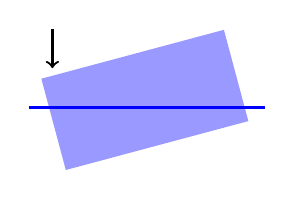
\begin{tikzpicture}

            \fill [blue!40, rotate around={15:(0,0.0)}] (-1.2,-0.5) rectangle (1.2,0.7);
            \draw[blue, thick] (-1.5,0) -- (1.5,0);
            \draw[black, thick, ->] (-1.2,1) -- (-1.2,0.5);
          
          \end{tikzpicture}
         \caption{The ship model is forces to an initial angle and then released}
         \label{fig:rolldecay_initial}
         \vspace{0.15cm}
     \end{subfigure}
     \hfill
     \begin{subfigure}[b,height=2cm]{0.22\textwidth}
         \centering
         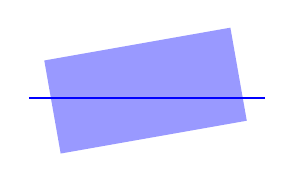
\begin{tikzpicture}

            \fill [blue!40, rotate around={10:(0,0.0)}] (-1.2,-0.5) rectangle (1.2,0.7);
            \draw[blue, thick] (-1.5,0) -- (1.5,0);
            
          \end{tikzpicture}
         \caption{Starts to roll back}
         \label{fig:rolldecay_free}
         \vspace{0.63cm}
     \end{subfigure}
     \hfill
     \begin{subfigure}[b,height=2cm]{0.22\textwidth}
         \centering
         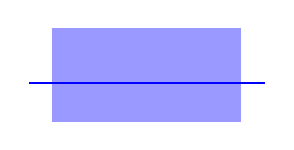
\begin{tikzpicture}

            \fill [blue!40, rotate around={0:(0,0.0)}] (-1.2,-0.5) rectangle (1.2,0.7);
            \draw[blue, thick] (-1.5,0) -- (1.5,0);
            
          \end{tikzpicture}
         \caption{Static water line.}
         \label{fig:rolldecay_equilibrium}
         \vspace{0.64cm}
     \end{subfigure}
    \hfill
     \begin{subfigure}[b,height=2cm]{0.22\textwidth}
         \centering
         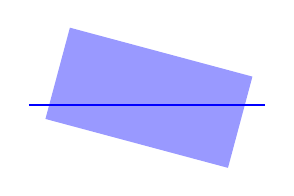
\begin{tikzpicture}

            \fill [blue!40, rotate around={-15:(0,0.0)}] (-1.2,-0.5) rectangle (1.2,0.7);
            \draw[blue, thick] (-1.5,0) -- (1.5,0);
            
          \end{tikzpicture}
         \caption{End point other side}
         \label{fig:rolldecay_endpoint}
         \vspace{0.36cm}
     \end{subfigure}
    \caption{Roll decay test.}
    \label{fig:rolldecay_procedure}
\end{figure}
\noindent This oscillation would never end if it was not for the roll damping. Interactions between the ship and the water, such as friction, wave generation, eddy generation, and hydrodynamic lift, will cause the ship to lose some of its energy. The energy loss means that the oscillation is decaying over time, as seen in \autoref{fig:rolldecay}, which displays the time series for the roll angle.

\begin{figure}[H]
    \centering
    \includegraphics[width=0.7\linewidth]{kappa/images/rolldecay_example.pdf}
    \caption{Example roll decay signal.}
    \label{fig:rolldecay}
\end{figure}

\noindent The damping $B_{44}\left(\dot{\phi}\right)$ can be expressed as an expansion series:  
\begin{equation}
    B_{44}\left(\dot{\phi}\right) = B_1\cdot\dot{\phi} + B_2\cdot\dot{\phi}\left|\dot{\phi}\right| + B_3\cdot\dot{\phi}^3 + ... + B_n\cdot\dot{\phi}^n
\end{equation}
 
\noindent This series can be truncated to be expressed as a ``linear model'' (\autoref{eq:roll_decay_equation_himeno_linear}), ``quadratic model'' (\autoref{eq:roll_decay_equation_himeno_quadratic_b}), and ``cubic model'' (\autoref{eq:roll_decay_equation_cubic}).

\input{equations/roll_decay_equation_himeno_linear}
\input{equations/roll_decay_equation_himeno_quadratic_b}
\input{equations/roll_decay_equation_cubic}
Models for the remaining degrees of freedom are presented in the next section.
\vspace{-0.2cm}
\section{Vessel manoeuvring models} \label{sec:manoeuvring model}
\label{\detokenize{02.01_manoeuvring models:vessel-manoeuvring-models}}\label{\detokenize{02.01_manoeuvring models:vmm}}\label{\detokenize{02.01_manoeuvring models::doc}}
\vspace{-0.2cm}
Ship manoeuvring is a simplified case of seakeeping. The encountering waves have been removed, assuming calm water conditions. The manoeuvring motions have low frequencies so that added masses and other hydrodynamic derivatives can be assumed as constants  \cite{fossen_handbook_2011}. Three manoeuvring models are used in this thesis: 
\begin{itemize}
    \item Linear (LVMM) \cite{matusiak_dynamics_2021}
    \item Abkowitz (AVMM) \cite{abkowitz_ship_1964}
    \item Modified Abkowitz (MAVMM), which is proposed in Paper \ref{pap:pit}
\end{itemize}

\noindent\autoref{\detokenize{02.01_manoeuvring models:coordinate-system}} shows the reference frames used in the manoeuvring models where \(x_0\) and \(y_0\) and heading \(\Psi\) are the global position and orientation of a ship fix reference frame \(O(x,y,z)\) (or rather \(O(x,y)\) when heave is excluded) with origin at midship. \(u\), \(v\), \(r\), \(X\), \(Y\) and \(N\) are velocities and forces in the ship fix reference frame.



\begin{figure}[H]
    \centering
    \includegraphics[width=0.8\textwidth]{kappa/images/coordinate_system.PNG}
    \caption{Reference frames.}
    \label{\detokenize{02.01_manoeuvring models:coordinate-system}}
\end{figure}

The manoeuvring equation can be described as \cite{fossen_handbook_2011},
\begin{equation}\label{equation:02.01_manoeuvring models:eqqsystem}
\begin{split}\displaystyle \left[\begin{matrix}- X_{\dot{u}} + m & 0 & 0\\0 & - Y_{\dot{v}} + m & - Y_{\dot{r}} + m x_{G}\\0 & - N_{\dot{v}} + m x_{G} & I_{z} - N_{\dot{r}}\end{matrix}\right] \left[\begin{matrix}\dot{u}\\\dot{v}\\\dot{r}\end{matrix}\right] = \left[\begin{matrix}m r^{2} x_{G} + m r v + \operatorname{X_{D}}{\left(u,v,r,\delta,thrust \right)}\\- m r u + \operatorname{Y_{D}}{\left(u,v,r,\delta,thrust \right)}\\- m r u x_{G} + \operatorname{N_{D}}{\left(u,v,r,\delta,thrust \right)}\end{matrix}\right]\end{split}
\end{equation}

\noindent where the first matrix describes the inertia of the ship in the surge, sway and yaw directions. The inertia in air is represented by the mass $m$ and moment of inertia $I_z$. The added mass in water is represented by: $X_{\dot{u}}$, $Y_{\dot{v}}$, $Y_{\dot{r}}$, $N_{\dot{v}}$ and $N_{\dot{r}}$. The hydrodynamic forces from the ship hull and rudder are desribed in the functions $X_D()$, $Y_D()$ and $N_D()$. The accelerations ($\dot{u}$, $\dot{v}$ and $\dot{r}$) can be solved from this equation,
\begin{equation}\label{equation:02.01_manoeuvring models:eqacc}
\begin{split}\displaystyle \dot{\nu} = \left[\begin{matrix}\dot{u}\\\dot{v}\\\dot{r}\end{matrix}\right] = \left[\begin{matrix}\frac{1}{- X_{\dot{u}} + m} & 0 & 0\\0 & - \frac{- I_{z} + N_{\dot{r}}}{S} & - \frac{- Y_{\dot{r}} + m x_{G}}{S}\\0 & - \frac{- N_{\dot{v}} + m x_{G}}{S} & - \frac{Y_{\dot{v}} - m}{S}\end{matrix}\right] \left[\begin{matrix}m r^{2} x_{G} + m r v + \operatorname{X_{D}}{\left(u,v,r,\delta,thrust \right)}\\- m r u + \operatorname{Y_{D}}{\left(u,v,r,\delta,thrust \right)}\\- m r u x_{G} + \operatorname{N_{D}}{\left(u,v,r,\delta,thrust \right)}\end{matrix}\right]\end{split}
\end{equation}

where \(S\) is a helper variable:
\begin{equation}\label{equation:02.01_manoeuvring models:eq_S}
\begin{split}\displaystyle S = - I_{z} Y_{\dot{v}} + I_{z} m + N_{\dot{r}} Y_{\dot{v}} - N_{\dot{r}} m - N_{\dot{v}} Y_{\dot{r}} + N_{\dot{v}} m x_{G} + Y_{\dot{r}} m x_{G} - m^{2} x_{G}^{2}\end{split}
\end{equation}


\noindent A state space model for manoeuvring can now be defined with six states:
\begin{equation}\label{equation:02.01_manoeuvring models:eq_x}
\begin{split}\displaystyle \mathbf{x} = \left[\begin{matrix}x_{0}\\y_{0}\\\Psi\\u\\v\\r\end{matrix}\right]\end{split}
\end{equation}
\noindent where $x_0$, $y_0$ and $\Psi$ are the global coordinates and heading of the ship and $u$, $v$ and $r$ are the velocities as seen in \autoref{\detokenize{02.01_manoeuvring models:coordinate-system}}.
The time derivative of this state \(\dot{\mathbf{x}}\) can be defined by a state transition \(f(\mathbf{x},\mathbf{c})\) using geometrical relations
how global coordinates \(x_0\), \(y_0\) and \(\Psi\) depend on \(u\), \(v\), and \(r\) viz.,
\begin{equation}\label{equation:02.01_manoeuvring models:eqf}
\begin{split}\displaystyle \dot{\mathbf{x}} = f(\mathbf{x},\mathbf{c}) + \mathbf{w}
                                          = \left[\begin{matrix}\dot{x_0}\\ \dot{y_0} \\ \dot{\Psi} \\\dot{u}\\\dot{v}\\\dot{r}\end{matrix}\right] + \mathbf{w}
                                          = \left[\begin{matrix}u \cos{\left(\Psi \right)} - v \sin{\left(\Psi \right)}\\u \sin{\left(\Psi \right)} + v \cos{\left(\Psi \right)}\\r\\\dot{u}\\\dot{v}\\\dot{r}\end{matrix}\right] + \mathbf{w}\end{split}
\end{equation}

where \(\mathbf{c}\) is control inputs (rudder angle \(\delta\) and thrust); the last three derivatives: \(\dot{u}\), \(\dot{v}\), \(\dot{r}\) are calculated with \autoref{equation:02.01_manoeuvring models:eqacc}.
\(\mathbf{w}\) is the process noise, i.e., the difference between the predicted state by the manoeuvring model and the true
state of the system. \(\mathbf{w}\) is unknown when the manoeuvring model is used for manoeuvre predictions and therefore normally
assumed to be zero, but it is an important factor when the manoeuvring model is used in the EKF (see \autoref{sec:datacleaning}).
The manoeuvring simulation can now be conducted by numerical integration of \autoref{equation:02.01_manoeuvring models:eqf}. The main difference between the manoeuvring model:s lies in how the hydrodynamic functions \(X_D(u,v,r,\delta,thrust)\), \(Y_D(u,v,r,\delta,thrust)\), \(N_D(u,v,r,\delta,thrust)\) are defined. These expressions are denoted in prime system ($X_D'$, $Y_D'$, $N_D'$) below for the various manoeuvring models: LVMM, AVMM and MAVMM.

\subsubsection*{{\normalfont \textbf{Linear vessel manoeuvring model (LVMM) \cite{matusiak_dynamics_2021}}}}
\begin{equation}\label{equation:02.01_manoeuvring models:eqxlinear}
\begin{split}\begin{split}
\operatorname{X_{D}'}{\left(u',v',r',\delta\right)} = & X_{\delta} \delta + X_{r} r' + X_{u} u' + X_{v} v' 
\end{split}\end{split}
\end{equation}\begin{equation}\label{equation:02.01_manoeuvring models:eqylinear}
\begin{split}\begin{split}
\operatorname{Y_{D}'}{\left(u',v',r',\delta \right)} = & Y_{\delta} \delta + Y_{r} r' + Y_{u} u' + Y_{v} v' 
\end{split}\end{split}
\end{equation}\begin{equation}\label{equation:02.01_manoeuvring models:eqnlinear}
\begin{split}\begin{split}
\operatorname{N_{D}'}{\left(u',v',r',\delta \right)} = & N_{\delta} \delta + N_{r} r' + N_{u} u' + N_{v} v' 
\end{split}\end{split}
\end{equation}

\subsubsection*{\normalfont \textbf{Abkowitz vessel manoeuvring model (AVMM) \cite{abkowitz_ship_1964}}}
\begin{equation}\label{equation:02.01_manoeuvring models:eqxabkowitz}
\begin{split}
\operatorname{X_{D}'}{\left(u',v',r',\delta,thrust' \right)} = & X_{\delta\delta} \delta^{2} + X_{r\delta} \delta r' + X_{rr} r'^{2} + X_{T} thrust' + X_{u\delta\delta} \delta^{2} u' \\ 
& + X_{ur\delta} \delta r' u' + X_{urr} r'^{2} u' + X_{uuu} u'^{3} + X_{uu} u'^{2} \\ 
& + X_{uv\delta} \delta u' v' + X_{uvr} r' u' v' + X_{uvv} u' v'^{2} \\
& + X_{u} u' + X_{v\delta} \delta v' + X_{vr} r' v' + X_{vv} v'^{2} 
\end{split}
\end{equation}

\begin{equation}\label{equation:02.01_manoeuvring models:eqyabkowitz}
\begin{split}\begin{split}
\operatorname{Y_{D}'}{\left(u',v',r',\delta,thrust' \right)} = & Y_{0uu} u'^{2} + Y_{0u} u' + Y_{0} + Y_{\delta\delta\delta} \delta^{3} + Y_{\delta} \delta + Y_{r\delta\delta} \delta^{2} r' + Y_{rr\delta} \delta r'^{2} \\ & + Y_{rrr} r'^{3} + Y_{r} r' + Y_{T\delta} \delta thrust' + Y_{T} thrust' + Y_{u\delta} \delta u' \\ & + Y_{ur} r' u' + Y_{uu\delta} \delta u'^{2} + Y_{uur} r' u'^{2} + Y_{uuv} u'^{2} v' + Y_{uv} u' v' \\ & + Y_{v\delta\delta} \delta^{2} v' + Y_{vr\delta} \delta r' v' + Y_{vrr} r'^{2} v' + Y_{vv\delta} \delta v'^{2} + Y_{vvr} r' v'^{2} \\ & + Y_{vvv} v'^{3} + Y_{v} v' 
\end{split}\end{split}
\end{equation}\begin{equation}\label{equation:02.01_manoeuvring models:eqnabkowitz}
\begin{split}\begin{split}
\operatorname{N_{D}'}{\left(u',v',r',\delta,thrust' \right)} = & N_{0uu} u'^{2} + N_{0u} u' + N_{0} + N_{\delta\delta\delta} \delta^{3} + N_{\delta} \delta + N_{r\delta\delta} \delta^{2} r' + N_{rr\delta} \delta r'^{2} \\ & + N_{rrr} r'^{3} + N_{r} r' + N_{T\delta} \delta thrust' + N_{T} thrust' + N_{u\delta} \delta u' \\ & + N_{ur} r' u' + N_{uu\delta} \delta u'^{2} + N_{uur} r' u'^{2} + N_{uuv} u'^{2} v' + N_{uv} u' v' \\ & + N_{v\delta\delta} \delta^{2} v' + N_{vr\delta} \delta r' v' + N_{vrr} r'^{2} v' + N_{vv\delta} \delta v'^{2} + N_{vvr} r' v'^{2} \\ & + N_{vvv} v'^{3} + N_{v} v' 
\end{split}\end{split}
\end{equation}

\subsubsection*{\normalfont \textbf{Modified Abkowitz vessel manoeuvring model (MAVMM)}}
\newline
Only the most relevant coefficients in AVMM are included, as proposed in Paper \ref{pap:pit}.
\begin{equation}\label{equation:02.01_manoeuvring models:eqxmartinssimple}
\begin{split}\begin{split}
\operatorname{X_{D}'}{\left(u',v',r',\delta,thrust' \right)} = & X_{\delta\delta} \delta^{2} + X_{rr} r'^{2} + X_{T} thrust' + X_{uu} u'^{2} + X_{u} u' + X_{vr} r' v' 
\end{split}\end{split}
\end{equation}\begin{equation}\label{equation:02.01_manoeuvring models:eqymartinssimple}
\begin{split}\begin{split}
\operatorname{Y_{D}'}{\left(u',v',r',\delta,thrust' \right)} = & Y_{\delta} \delta + Y_{r} r' + Y_{T\delta} \delta thrust' + Y_{T} thrust' + Y_{ur} r' u' + Y_{u} u' \\ & + Y_{vv\delta} \delta v'^{2} + Y_{v} v' 
\end{split}\end{split}
\end{equation}\begin{equation}\label{equation:02.01_manoeuvring models:eqnmartinssimple}
\begin{split}\begin{split}
\operatorname{N_{D}'}{\left(u',v',r',\delta,thrust' \right)} = & N_{\delta} \delta + N_{r} r' + N_{T\delta} \delta thrust' + N_{T} thrust' + N_{ur} r' u' + N_{u} u' \\ & + N_{vv\delta} \delta v'^{2} + N_{v} v' 
\end{split}\end{split}
\end{equation}

The hydrodynamic functions above are expressed using nondimensional units with the prime system, denoted by the prime symbol (\('\)). The quantities are expressed in the prime system, using the denominators in \autoref{tab:prime-system-denominators}. For instance, surge linear velocity \(u\) can be expressed in the prime system as seen in \autoref{equation:02.01_manoeuvring models:eqprime} using the linear velocity denominator.
\begin{equation}\label{equation:02.01_manoeuvring models:eqprime}
\begin{split}\displaystyle u'=\frac{u}{V}\end{split}
\end{equation}

Equations can either be written in the Prime or regular Standard Institute (SI) system. The hydrodynamic derivatives are always expressing forces in the prime system as function of state variables. The (\('\)) sign is therefore implicit and not written out as seen in \autoref{equation:02.01_manoeuvring models:eqderivativeprime}.
\begin{equation}\label{equation:02.01_manoeuvring models:eqderivativeprime}
\begin{split}\displaystyle Y_{\delta'}'=\frac{\partial Y_D'}{\partial \delta'} := Y_{\delta} \end{split}
\end{equation}

The exceptions are the added masses (\(X_{\dot{u}}\), \(Y_{\dot{v}}\), \(Y_{\dot{r}}\), \(N_{\dot{v}}\) and \(N_{\dot{r}}\)) which are expressed in both Prime system or the regular SI system where the (\('\)) sign is therefore
explicitly stated.
There is however a great benefit in expressing the hydrodynamic forces in the prime system. The forces are often nonlinear due to a quadratic relation to the flow velocity, as seen in \autoref{equation:02.01_manoeuvring models:eqquadraticsi}.
\begin{equation}\label{equation:02.01_manoeuvring models:eqquadraticsi}
\begin{split}\displaystyle Y_{D}=Y_{\delta} \cdot \delta \cdot \frac{L^2V^2\rho}{2}\end{split}
\end{equation}
which becomes linear when expressed in the prime system as seen in \autoref{equation:02.01_manoeuvring models:eqquadraticprime}.
\begin{equation}\label{equation:02.01_manoeuvring models:eqquadraticprime}
\begin{split}\displaystyle Y_{D}'=Y_{\delta} \cdot \delta'\end{split}
\end{equation}
\subsection{The propeller model}
\label{\detokenize{02.10_propeller_model:the-propeller-model}}\label{\detokenize{02.10_propeller_model::doc}}
\sphinxAtStartPar
A propeller model is developed based on Manoeuvring Modeling Group (MMG) model \cite{yasukawa_introduction_2015} where the thrust is expressed as:
\begin{equation}\label{equation:02.10_propeller_model:eqT}
\begin{split}\displaystyle thrust = D^{4} K_{T} n^{2} \rho\end{split}
\end{equation}
\sphinxAtStartPar
and the thrust coefficient \(K_T\) is modelled as a second order polynomial:
\begin{equation}\label{equation:02.10_propeller_model:eqkt}
\begin{split}\displaystyle K_{T} = J^{2} k_{2} + J k_{1} + k_{0}\end{split}
\end{equation}
\sphinxAtStartPar
The advance ratio \(J\) is calculated as:
\begin{equation}\label{equation:02.10_propeller_model:eqJ}
\begin{split}\displaystyle J = \frac{u \left(1 - w_{p}\right)}{D n}\end{split}
\end{equation}
\sphinxAtStartPar
where \(D\) is propeller diameter, \(n\) is propeller speed and \(w_p\) is the wake fraction at an oblique inflow to the propeller from the drift angle and the yaw rate. A semi\sphinxhyphen{}empirical formula for \(w_p\) is provided in the MMG model. As an alternative, a simple polynomial is proposed in \autoref{equation:02.10_propeller_model:eqpropellermodel}.
\begin{equation}\label{equation:02.10_propeller_model:eqpropellermodel}
\begin{split}\displaystyle w_{p} = C_{1} \delta + C_{2} \delta^{2} + C_{3} \beta_{p}^{2} + C_{4} u + w_{p0}\end{split}
\end{equation}
\sphinxAtStartPar
\(w_p\) is modeled as a function of rudder angle \(\delta\), to include wake influence from the rudder and ship speed \(u\), to include a speed dependency. The influence from drift angle \(\beta\) and yaw rate \(r\) is expressed by \(\beta_p\) in \autoref{equation:02.10_propeller_model:eqbetap}.
\begin{equation}\label{equation:02.10_propeller_model:eqbetap}
\begin{split}\beta_p=\beta - \frac{r}{V} \cdot x_p \end{split}
\end{equation}
where \(x_p\) is the propeller longitudinal position and \(w_{p0}\) is the regular Taylor wake fraction, applicable to straight ahead steaming with no rudder angle. Similar to the MMG propeller model, two sets of parameters \(C_1\)-\(C_4\) should be used in the propeller model depending on the sign of \(\beta_p\).
\subsection{Prime system} \label{sec:prime_system}
Some variables in the equations in this paper are expressed using nondimensional units with the prime system, denoted by the prime symbol ($'$). Variables are converted from SI units to the prime system using the denominators in \autoref{tab:prime_system} for the corresponding physical quantity, where $U$ and $L$ are the velocity and length between the perpendiculars of the ship, respectively, and $\rho$ is the water density.
For the calculation of surge velocity $u'$, the perturbed velocity $(u-U_0)$ about a nominal speed $U_0$ is used, as in \autoref{eq:u_prime}, to avoid a $u'$ of 1 for all speeds when the ship is on a straight course (where $u=U$), as in a resistance or self-propulsion test. The usage of the perturbed velocity, therefore, allows for higher order resistance terms in the model, such as $X_{u}$, which are otherwise not possible. 
\begin{equation}
    \label{eq:u_prime}
    u' = \frac{u-U_0}{U}
\end{equation}
For a nondimensional model, $U_0$ is instead expressed as a Froude number within the model (\autoref{eq:Fn0}), and this paper uses $F_{n0}=0.02$.
\begin{equation}
    \label{eq:Fn0}
    F_{n0} = \frac{U_0}{\sqrt{g \cdot L}}
\end{equation}
\begin{table}[h]
    \centering
    \caption{Scalings with prime system.}
    \label{tab:prime_system}
    \pgfplotstabletypeset[col sep=comma,
        columns={Physical quantity,SI unit,Denominator},
        columns/SI unit/.style={string type},
        columns/Physical quantity/.style={string type},
        columns/Denominator/.style={string type},
        column type=l,	% specify the align method
        every head row/.style={before row=\hline,after row=\hline},	% style the first row
        every last row/.style={after row=\hline},	% style the last row
    ]{tables/prime_system.prime_system.csv"}
\end{table}
%%%%%%%%%%%%%%%%%%%%%%%%%%%%%%%
%%%%%%%%%%%%%%%%%%%%%%%%%%%%%%%
\chapter{Parameter identification}\label{ch:methods}
%%%%%%%%%%%%%%%%%%%%%%%%%%%%%%%
%Section comments: There were more changes related to objective language and directional words. There is a missing term near line 13.
The system identification of rigid body ship dynamics can be simplified into parameter estimation if parameterized physical models is assumed as the most appropriate model from a collection of candidate models.
The parameter estimations for roll motion and manoeuvring are presented in \autoref{sec:_roll} and \autoref{sec:RIDR}. The most appropriate models are selected in the model development process described in \autoref{sec:cross_validation}.

\section{Roll model parameter estimation} \label{sec:_roll}
\noindent Damping parameters can be estimated directly from the VCT forces, as demonstrated in \autoref{sec:VCT}. However, this approach is not feasible when the ship is free to move, necessitating the use of FT time series data to estimate the parameters. In such cases, the entire dynamics must be considered. The damping parameters ($B_1$, $B_2$, $B_3$) and stiffness parameters ($C_1$, $C_3$, $C_5$) can be identified from the parametric linear, quadratic, and cubic roll motion model structures presented in the previous chapter (\autoref{eq:roll_decay_equation_himeno_linear}, \autoref{eq:roll_decay_equation_himeno_quadratic_b}, and \autoref{eq:roll_decay_equation_cubic}).
These equations do not have unique solutions because each equation can be multiplied by an arbitrary factor to yield a new valid solution. To obtain unique solutions, inertia is excluded by normalizing the equations with the total roll inertia $A_{44}$, as shown in \autoref{eq:roll_decay_nonedim_a44} for the linear model.

\input{equations/roll_decay_nonedim_A44}

\noindent The identified normalized damping and stiffness parameters $B_{1A}$ and $C_{1A}$ can be expressed in dimensional units by multiplication with the normalization factor $A_{44}$. If $A_{44}$ is unknown before hand, it can be calculated using \autoref{eq:A_44_eq} \cite{piehlShipRollDamping2016}, assuming that the meta center height $GM$ is known.
\input{equations/A_44_eq}
The frequency $\omega_0$ can be obtained with fast Fourier transform (FFT) of the roll signal. 
Two methods for parameter estimation have been investigated: the \say{derivation approach}, referred to in \textcite{imo1200InterimGuidelines2006}, and the \say{integration approach} used in \textcite{soderAssessmentShipRoll2019} which are both described in the next subsections. 

%\subsection{Inverse dynamics regression}\label{sec:derivation_approach}
In inverse dynamics regression (called derivation approach in Paper \ref{pap:rolldamping}), \autoref{eq:roll_decay_nonedim_a44} is treated as a linear regression problem, where the states ($\phi$, $\dot{\phi}$, $\ddot{\phi}$) are known and the parameters $B_1$ and $C_1$ must be regressed. Only roll angle $\phi$ is known from the experimental data, which means that the velocity and acceleration $\dot{\phi}$, $\ddot{\phi}$ also must be approximated (note that this is done with numerical differentiation in Paper \ref{pap:rolldamping} and with the extended Kalman filter (EKF) in Paper \ref{pap:pit}).
A least squares fit is applied to the roll motion equation to identify the damping and stiffness parameters.

%\subsection{Integration approach}\label{sec:integration_approach}
In the integration approach, \autoref{eq:roll_decay_nonedim_a44} is solved as an ordinary differential equation (ODE) for many estimated sets of parameters until the solution converges. This method is time-consuming, and convergence is not guaranteed. However, the advantage is that only roll angle $\phi$ is needed.
\section{Parameter estimation from virtual captive tests} \label{sec:VCT}
The computational cost of CFD calculations can be significantly reduced by assuming a memory-less state space model (\autoref{eq:state_space}), also known as the Markov process assumption \cite{yoonIdentificationHydrodynamicCoefficients2003}. This assumption implies that the forces acting on the ship at each time instant can be constructed as a series of independent static flow calculations.

The independence of these static flow calculations means they are not time-dependent, and their order of computation is irrelevant. The Markov process assumption allows for substantial computational efficiency gains because the ship experiences the same state $\mathbf{x}$ and input $\mathbf{u}$ (or very similar states and inputs) multiple times during a maneuver. Consequently, the same static flow result can be reused several times, or at least conceptually, this reuse can be considered. Practically, this is achieved by identifying a prediction model for the static flow results, the VCT data, so that forces for each state during the maneuver can be predicted.

One of the challenges with VCT is selecting appropriate static flow calculations. This involves creating a VCT matrix that includes the most critical states during the maneuver, covering the relevant parts of the state space.

The ship's kinematics are defined by the velocity vector $\pmb{\bm{\upsilon}}$ and the input vector $\mathbf{u}$, allowing the forces for each state to be uniquely defined by the velocities $u$, $v$, and $r$, as well as the input forces from the rudder and propeller. If these forces are uniquely determined by the thrust and rudder angle, the state space spans at least five dimensions, which requires numerous VCT calculations to cover the entire state space.

Another challenge with VCT is selecting a model structure that closely resembles the true hydrodynamics, ensuring high accuracy without having to span the entire state space.
\autoref{tab:VCT_wPCC} and \autoref{tab:VCT_optiwise} present the VCT matrices for the wPCC and Optiwise test cases. The coverage of the yaw rate and drift angle space is illustrated by the phase plots in \autoref{fig:phase_plots}.
% wPCC
\begin{table}[h]
    \centering
    \small
    \caption{State variations with VCT for wPCC.}
    \label{tab:VCT_wPCC}
    \pgfplotstabletypeset[col sep=comma, column type=c, style=string type,
        columns/Test type/.style={column type=l,string type},
        columns/V/.style={column type=c,string type, column name=$V$ [m/s]},
        columns/beta_deg/.style={column type=c,string type, column name=$\beta$ [deg]},
        columns/r/.style={column type=c,string type, column name=$r$ [rad/s]},
        columns/delta_deg/.style={column type=c,string type, column name=$\delta$ [deg]},
        columns/rev/.style={column type=c,string type, column name=rev [1/s]},
        %columns/r/.style={column type=r,fixed,fixed zerofill,precision=2, column name=$r$ [rad/s]},
        %columns/V_R/.style={fixed,fixed zerofill,precision=2, column name=$V_R$ [m/s]},
        %columns/gamma_deg/.style={fixed,fixed zerofill,precision=1, column name=$\gamma$ [deg]},
        %columns/Y_R/.style={fixed,fixed zerofill,precision=1, column name=$Y_R^{VCT}$ [N]},
        %columns/Y_R_MMG/.style={fixed,fixed zerofill,precision=1, column name=$Y_R^{MMG}$ [N]},
        every head row/.style={before row=\hline,after row=\hline},
        every last row/.style={after row=\hline}
    ]{tables/methodology_VCT_wPCC.variations.csv}
\end{table}
% Optiwise
\begin{table}[h]
    \centering
    \small
    \caption{State variations with VCT for Optiwise.}
    \label{tab:VCT_optiwise}
    \pgfplotstabletypeset[col sep=comma, column type=c, style=string type,
        columns/Test type/.style={column type=l,string type},
        columns/V/.style={column type=c,string type, column name=$V$ [m/s]},
        columns/beta_deg/.style={column type=c,string type, column name=$\beta$ [deg]},
        columns/r/.style={column type=c,string type, column name=$r$ [rad/s]},
        columns/delta_deg/.style={column type=c,string type, column name=$\delta$ [deg]},
        columns/rev/.style={column type=c,string type, column name=rev [1/s]},
        %columns/r/.style={column type=r,fixed,fixed zerofill,precision=2, column name=$r$ [rad/s]},
        %columns/V_R/.style={fixed,fixed zerofill,precision=2, column name=$V_R$ [m/s]},
        %columns/gamma_deg/.style={fixed,fixed zerofill,precision=1, column name=$\gamma$ [deg]},
        %columns/Y_R/.style={fixed,fixed zerofill,precision=1, column name=$Y_R^{VCT}$ [N]},
        %columns/Y_R_MMG/.style={fixed,fixed zerofill,precision=1, column name=$Y_R^{MMG}$ [N]},
        every head row/.style={before row=\hline,after row=\hline},
        every last row/.style={after row=\hline}
    ]{tables/methodology_VCT_optiwise.variations.csv}
\end{table}
\begin{figure}[H]
     \centering
     \begin{subfigure}[b]{0.49\textwidth}
         \centering
         \includesvg[width=0.99\textwidth]{figures/methodology_VCT_wPCC.phase_plot.svg}
        \caption{wPCC.}
        \label{fig:VCT_phase_plot_wPCC}
     \end{subfigure}
     \hfill
     \begin{subfigure}[b]{0.49\textwidth}
        \centering
        \includesvg[width=0.99\textwidth]{figures/methodology_VCT_optiwise.phase_plot.svg}
        \caption{Optiwise.}
        \label{fig:VCT_phase_plot_optiwise}
     \end{subfigure}
        \caption{Phase plots of the zigzag tests together with the coverage of the VCTs and extra state VCTs.}
        \label{fig:phase_plots}
\end{figure}

The hydrodynamic damping forces are calculated from the VCT results $X_{VCT}$, $Y_{VCT}$ and $N_{VCT}$
with \autoref{eq:X_D} -- \autoref{eq:N_D}.
\begin{equation}
    \label{eq:X_D}
    X_{D} = X_{VCT} + Y_{\dot{r}} r^{2} + Y_{\dot{v}} r v
\end{equation}
\begin{equation}
    \label{eq:Y_D}
    Y_{D} = - X_{\dot{u}} r u + Y_{VCT}
\end{equation}
\begin{equation}
    \label{eq:N_D}
    N_{D} = N_{VCT} + X_{\dot{u}} u v - Y_{\dot{r}} r u - Y_{\dot{v}} u v
\end{equation}
The mass $m$ has disappeared from \autoref{eq:F_expanded} to arrive at these expressions, because the ship is not moving in ShipFlow -- the CFD tool used in the static flow calculations -- instead the water is having an either oblique or circular inflow \cite{roychoudhuryCFDSimulationsSteady2017}.
The hull forces are calculated by subtracting the contributions of the rudder and propeller from the total forces (\autoref{eq:X_H_VCT} -- \autoref{eq:N_H_VCT}).
\begin{equation}
    \label{eq:X_H_VCT}
    X_H = X_D - X_R - X_P
\end{equation}
\begin{equation}
    \label{eq:Y_H_VCT}
    Y_H = Y_D - Y_R
\end{equation}
\begin{equation}
    \label{eq:N_H_VCT}
    N_H = N_D - N_R
\end{equation}
These forces are used together with the hull force model (\autoref{eq:X_H} -- \autoref{eq:N_H}) to define a linear regression problem that is solved with the ordinary least squares (OLS) method. 
\section{Inverse dynamics} \label{sec:ID}
Inverse dynamics (ID) is a widely used technique in robotics \cite{faberInverseDynamicsMechanical2018, haningerNonparametricInverseDynamic2019, mastalliInverseDynamicsMPCNullspace2023, sunHighorderInverseDynamics2023, kurtzInverseDynamicsTrajectory2023} that is also well applicable to ship dynamics. It can be used to estimate the total forces that act on a ship during motion. The technique can be applied to data from free-model manoeuvring tests or real ship maneuvers. The forces acting on the ship during a maneuver can be estimated with inverse dynamics of the equation of motion (\autoref{eq:eom}) when the mass matrix $\mathbf{M}$ and the acceleration vector $\pmb{\bm{\dot{\upsilon}}}$ are known. The hydrodynamic damping forces can be calculated by inserting the total force $\mathbf{F}$ from \autoref{eq:F_expanded} into \autoref{eq:eom} and then solving for $X_D$, $Y_D$, and $N_D$ as shown in \autoref{eq:ID_X}-\autoref{eq:ID_N}.
\begin{equation}
    \label{eq:ID_X}
    \input{equations/methodology_ID.X_D}
\end{equation}
\begin{equation}
    \label{eq:ID_Y}
    \input{equations/methodology_ID.Y_D}
\end{equation}
\begin{equation}
    \label{eq:ID_N}
    \input{equations/methodology_ID.N_D}
\end{equation}
These expressions are used to estimate the forces acting on the ship during FRMTs, for instance as shown for a turning circle test in \autoref{fig:ID}.
\begin{figure}[H]
    \centering
    \includegraphics[width=\textwidth]{kappa/images/1.pdf}
    \caption{Forces and moments calculated with inverse dynamics on data from a turning circle test.}
    \label{fig:ID}
\end{figure}

The estimated inverse dynamics forces were used in Paper \ref{pap:pit} and \ref{pap:physics} as input to an inverse dynamics regression (see \autoref{sec:IDR}). 
Inverse dynamics was also used in Paper \ref{pap:physics} and \ref{pap:vct} to estimate the forces acting on the ship during the FRMTs to be compared with the model force predictions. This is a more informative way to assess model performance than, for instance, using open-loop or closed-loop simulations. The benefit is that the model and the experiment will always be in the same state, which is not the case when simulations are used.
\section{Inverse dynamics regression} \label{sec:IDR}
Parameter estimation from CMT or VCT is the classic way to identify parameters within a manoeuvring model. However, a model can also be identified from time series obtained with FRMTs or full-scale maneuvers. Instead of, as in the CMT or VCT, having direct measured forces, the forces can instead be estimated with inverse dynamics (see \autoref{sec:ID}). 


\section{Added mass estimation with the Fourier series method}
\label{sec:fourier}
The yaw added mass $N_{\dot{r}}$ was determined with the Fourier series method \cite{sakamoto_cfd_2021} applied on a pure yaw test conducted in a a fully nonlinear potential flow (FNPF) panel method in ShipFlow Motions (Motions) \cite{kjellberg_fully_2013}.
During the pure yaw test the heading $\Psi$ was varied according to \autoref{eq:pure_yaw_psi} so that the yaw rate $r$ and yaw acceleration $\dot{r}$ were varied according to \autoref{eq:pure_yaw_r}, and \autoref{eq:pure_yaw_r1d}.
\begin{equation}
    \Psi = - \Psi_{max} \cos{\left(t w \right)}
    \label{eq:pure_yaw_psi}
\end{equation}
\begin{equation}
    r = \Psi_{max} w \sin{\left(t w \right)}
    \label{eq:pure_yaw_r}
\end{equation}
\begin{equation}
    \dot{r} = \Psi_{max} w^{2} \cos{\left(t w \right)}
    \label{eq:pure_yaw_r1d}
\end{equation}
The pure yaw calculations in Motions were conducted without propeller and rudder so that $N_D=N_H$ and the moment equilibrium with the yawing moment from the pressure integration in Motions $N_M$ could be expressed with \autoref{eq:MOTIONS_N}, where the yaw added mass $N_{\dot{r}}$ was the coefficient of interest. 
\begin{equation}
    \input{equations/methodology_pure_yaw_no_FFT.MOTIONS_N.tex}
    \label{eq:MOTIONS_N}
\end{equation}
The time series for the yawing moment during the pure yaw test could thus be expressed by inserting \autoref{eq:pure_yaw_psi} -- \autoref{eq:pure_yaw_r1d} into \autoref{eq:MOTIONS_N} as shown in \autoref{eq:MOTIONS_N_expanded}.
\begin{equation}
    %\input{equations/methodology_pure_yaw_no_FFT.MOTIONS_N_expanded}
    \begin{align}    
    N_{M} = N_{\dot{r}} \Psi_{max} w^{2} \cos{\left(t w \right)} + N_{rrr} \Psi_{max}^{3} w^{3} \sin^{3}{\left(t w \right)} + \\ 
    N_{r} \Psi_{max} w \sin{\left(t w \right)} + Y_{\dot{r}} \Psi_{max} u w \sin{\left(t w \right)}
    \end{align}
    \label{eq:MOTIONS_N_expanded}
\end{equation}
\autoref{eq:MOTIONS_N_expanded} can instead be expressed as a Fourier series with three components as shown in \autoref{eq:fourier} where $N_{\dot{r}}$ can be calculated from the first cosine coefficient (\autoref{eq:N_r1d}).
\begin{equation}
    N_M = N_0 + \sum_{n=1}^3a_n \cos(n \omega t) + \sum_{n=1}^3b_n \sin(n \omega t) 
    \label{eq:fourier}
\end{equation}
\begin{equation}
    N_{\dot{r}} = \frac{a_1}{\Psi_{max} w^{2}}
    \label{eq:N_r1d}
\end{equation}
An example of the fitted Fourier series is shown in \autoref{fig:fourier}. The sway added mass $Y_{\dot{v}}$ was determined in a similar way, but instead by conducting a pure sway test. The coupled added masses $N_{\dot{v}}$, and $Y_{\dot{r}}$ were determined with strip theory calculations using Franks close fit method.
\begin{figure}[h]
    \centering
    \begin{subfigure}[b]{0.49\textwidth}
        \includesvg[width=0.99\textwidth]{figures/methodology_pure_yaw_no_FFT.track_plot.svg}
        \caption{Track plot.}
    \end{subfigure}
    \hfill
    \begin{subfigure}[b]{0.49\textwidth}
        \includesvg[width=0.99\textwidth]{figures/methodology_pure_yaw_no_FFT.reconstruction.svg}
        \caption{Fourier series fit.}
    \end{subfigure}
    \caption{Pure yaw ShipFlow Motions results to determine the yaw added mass.}
    \label{fig:fourier}
\end{figure}
%\section{Manoeuvring model parameter estimation} \label{sec:RIDR}
A new parameter estimation method is proposed in Paper \ref{pap:pit} for the remaining degrees of freedom. A manoeuvring model is used to solve the reversed manoeuvring problem. The problem may consist of predicting unknown forces from known manoeuvring model test data. The hydrodynamic derivatives in the manoeuvring model can be identified through regression of the force polynomials on forces predicted with inverse dynamics (see \autoref{\detokenize{03.01_inverse_dynamics::doc}}).
The measurement noise must be removed prior to the regression of hydrodynamic derivatives in the manoeuvring model. This is conducted by an extended Kalman filter (EKF) and a Rauch Tung Striebel (RTS) smoother (see \autoref{sec:datacleaning}). The EKF requires an accurate manoeuvring model as the predictor.
Therefore, the accurate manoeuvring model is both the input and output of the method. As a solution to this dilemma, a linear manoeuvring model that includes hydrodynamic derivatives estimated with semi-empirical formulas (\autoref{app:initial_estimates}) is used as the initial predictor. Once the regressed manoeuvring model has been obtained, the parameter estimation can be refined, using the regressed manoeuvring model as the predictor model in the EKF, to improve the filter and obtain a more accurate manoeuvring model. The method is summarized in \autoref{fig:greyvmm} and can be repeated several times (indicated by the dashed arrow) for improved accuracy. 
\begin{figure}[h]
    
    \centering
    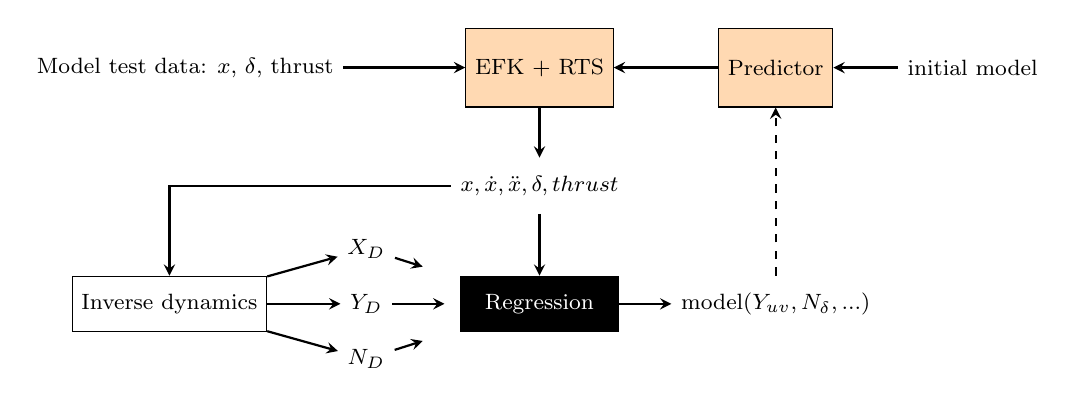
\begin{tikzpicture}[node distance=1.5cm]
    %\draw (0,0) rectangle (10,10); %create a bounding box to reserve space
    \node (data) [io] {\footnotesize Model test data: $x$, $\delta$, thrust};
    
    \node (EKF) [process, right of=data, xshift=3.0cm] {\footnotesize EFK + RTS};
    \node (predictor) [process, right of=EKF, xshift=1.5cm]{\footnotesize Predictor};
    \node (VMM) [io, right of=predictor, xshift=1.0cm] {\footnotesize initial model};
    
    \node (data_clean) [io, below of=EKF] {\footnotesize \(x,\dot{x},\ddot{x}, \delta, thrust\)};
    
    \node (black-box) [black-box, below of=data_clean] {\footnotesize Regression};
    
    \node (X_D) [io, left of=black-box, xshift=-0.70cm, yshift=0.7cm]{\footnotesize \(X_D\)};
    \node (Y_D) [io, left of=black-box, xshift=-0.70cm, yshift=0cm]{\footnotesize \(Y_D\)};
    \node (N_D) [io, left of=black-box, xshift=-0.70cm, yshift=-0.7cm]{\footnotesize \(N_D\)};
    
    \node (white-box) [white-box, left of=Y_D, xshift=-1.00cm] {\footnotesize Inverse dynamics};
    
    
    %
    %
    \node (coefficients) [io, right of=black-box, xshift=1.5cm] {\footnotesize model$\left(Y_{uv},N_{\delta},...\right)$};
    
    \draw [arrow] (data) -- (EKF);
    \draw [arrow] (predictor) -- (EKF);
    \draw [arrow] (VMM) -- (predictor);
    \draw [arrow] (EKF) -- (data_clean);
    
    \draw [arrow] (data_clean) -| (white-box);
    \draw [arrow] (data_clean) -- (black-box);
    
    \draw [arrow] (white-box) -- (X_D);
    \draw [arrow] (white-box) -- (Y_D);
    \draw [arrow] (white-box) -- (N_D);
    
    \draw [arrow, shorten >=0.5cm] (X_D) -- (black-box);
    \draw [arrow, shorten >=0.2cm] (Y_D)  -- (black-box);
    \draw [arrow, shorten >=0.5cm] (N_D)  -- (black-box);
    
    
    \draw [arrow] (black-box)  -- (coefficients);
    \draw [arrow, dashed] (coefficients)  -- (predictor);
    
    \end{tikzpicture}
    \caption{Method to estimate the manoeuvring model hydrodynamic derivatives.}
    \label{fig:greyvmm}
\end{figure}

\noindent Using semi-empirical formulas (\autoref{app:initial_estimates}) for the initially estimated manoeuvring model adds prior knowledge about the ship dynamics to the regression. An example, with simulation results from the steps in the iteration, is presented in \hyperref[\detokenize{01.01_method:iterations}]{\autoref{\detokenize{01.01_method:iterations}}}.


\begin{figure}[H]
    \centering
    \includegraphics[width=\textwidth]{kappa/images/0.pdf}
    \caption{Simulation with: initial model and first and second iteration of the parameter estimation method.}
    \label{\detokenize{01.01_method:iterations}}
\end{figure}

\subsection{Inverse dynamics and regression}
\label{\detokenize{03.01_inverse_dynamics:inverse-dynamics-and-regression}}\label{\detokenize{03.01_inverse_dynamics::doc}}

Each manoeuvring model has some hydrodynamic functions \(X_D(u,v,r,\delta,thrust)\), \(Y_D(u,v,r,\delta,thrust)\), \(N_D(u,v,r,\delta,thrust)\) that are defined as polynomials. The hydrodynamic derivatives in these polynomials can be identified with force regression of measured forces and moments. The measured forces and moments are usually taken from captive model tests (CMT), planar motion mechanism (PMM) tests, or virtual captive tests (VCT). However, motions are recorded when the ship is free in all degrees of freedom. Hence, forces and moments causing ship motion must be estimated by solving the inverse dynamics problem.
The inverse dynamics problem is solved by restructuring the system equation (\autoref{equation:02.01_manoeuvring models:eqacc}) to get the hydrodynamics functions on the left-hand side. If the mass and inertia of the ship with added masses: \(X_{\dot{u}}\), \(Y_{\dot{v}}\), \(Y_{\dot{r}}\), \(N_{\dot{v}}\), and \(N_{\dot{r}}\) are known; the forces in the Prime system can be calculated using \autoref{equation:03.01_inverse_dynamics:eqxd}, \autoref{equation:03.01_inverse_dynamics:eqyd}, and \autoref{equation:03.01_inverse_dynamics:eqnd}.
These forces can be used to regress the hydrodynamic derivatives through the ordinary least square (OLS) method. If the added masses are unknown, they can be calculated using potential flow methods or semi-empirical methods (\autoref{app:initial_estimates}). 
\begin{equation}\label{equation:03.01_inverse_dynamics:eqxd}
\begin{split}\displaystyle \operatorname{X_{D}'}{\left(u',v',r',\delta,thrust' \right)} = - X_{\dot{u}}' \dot{u}' + \dot{u}' m' - m' r'^{2} x_{G}' - m' r' v'\end{split}
\end{equation}\begin{equation}\label{equation:03.01_inverse_dynamics:eqyd}
\begin{split}\displaystyle \operatorname{Y_{D}'}{\left(u',v',r',\delta,thrust' \right)} = - Y_{\dot{r}}' \dot{r}' - Y_{\dot{v}}' \dot{v}' + \dot{r}' m' x_{G}' + \dot{v}' m' + m' r' u'\end{split}
\end{equation}\begin{equation}\label{equation:03.01_inverse_dynamics:eqnd}
\begin{split}\displaystyle \operatorname{N_{D}'}{\left(u',v',r',\delta,thrust' \right)} = I_{z}' \dot{r}' - N_{\dot{r}}' \dot{r}' - N_{\dot{v}}' \dot{v}' + \dot{v}' m' x_{G}' + m' r' u' x_{G}'\end{split}
\end{equation}

\noindent An example that includes forces calculated with inverse dynamics from motions in a turning circle test can be seen in \hyperref[\detokenize{03.01_inverse_dynamics:fig-inverse}]{\autoref{\detokenize{03.01_inverse_dynamics:fig-inverse}}}. The forces have been converted to SI units.

\begin{figure}[H]
    \centering
    \includegraphics[width=\textwidth]{kappa/images/1.pdf}
    \caption{Forces and moments calculated with inverse dynamics on data from a turning circle test.}
    \label{\detokenize{03.01_inverse_dynamics:fig-inverse}}
\end{figure}
%\subsection{Inverse dynamics regression} \label{sec:IDR}
Finding the hydrodynamic derivatives can be defined as a linear regression problem following the ''derivation approach'' (see \autoref{sec:derivation_approach}):
\begin{equation}\label{equation:03.01_inverse_dynamics:eqregression}
\begin{split}y = X\gamma + \epsilon\end{split}
\end{equation}

\noindent The label vector \(y\) and feature matrix \(X\) in the regression problem in \autoref{equation:03.01_inverse_dynamics:eqregression} can be calculated if model for the hydrodynamic forces is assumed. For example: the label in the regression of the surge degree of freedom for the MAVMM can be calculated using the inverse dynamics force, which is expressed with primed units:
\begin{equation}\label{equation:03.01_inverse_dynamics:diff_eq_X_y}
\begin{split}\displaystyle y = - X_{\dot{u}} \dot{u}' + \dot{u}' m' - m' r'^{2} x_{G'} - m' r' v'\end{split}
\end{equation}

\noindent The feature matrix \(X\) is expressed as:
\begin{equation}\label{equation:03.01_inverse_dynamics:diff_eq_X_X}
\begin{split}\displaystyle X = \left[\begin{matrix}thrust' & u' & \delta^{2} & r'^{2} & u'^{2} & r' v'\end{matrix}\right]\end{split}
\end{equation}

\noindent The hydrodynamic derivatives in the \(\gamma\) vector (\autoref{equation:03.01_inverse_dynamics:diff_eq_X_beta}) can be estimated with ordinary least squares (OLS) regression.
\begin{equation}\label{equation:03.01_inverse_dynamics:diff_eq_X_beta}
\begin{split}\displaystyle \gamma = \left[\begin{matrix}X_{T}\\X_{u}\\X_{\delta\delta}\\X_{rr}\\X_{uu}\\X_{vr}\end{matrix}\right]\end{split}
\end{equation}
In this regression, the hydrodynamic derivatives are treated as Gaussian random variables. The hydrodynamic derivatives in the manoeuvring model are usually estimated as the mean value of each regressed random variable, which is the most likely estimate. The regression result can be expressed with a multivariate Gaussian distribution, which is defined by the regression’s mean values and covariance matrix. The multivariate Gaussian distribution can be used to conduct Monte Carlo simulations in the study of alternative realizations of the regression.

Strong multicollinearity is a documented problem for the manoeuvring models \cite{luo_parameter_2016, wang_quantifying_2018}.
The thrust coefficient \(X_T\) in the hydrodynamic function \(X_D\) in \autoref{equation:02.01_manoeuvring models:eqxabkowitz} introduces multicollinearity to the regression. This coefficient can instead be calculated from the thrust deduction factor \(t_{df}\):
\begin{equation}\label{equation:03.01_inverse_dynamics:eqXthrust}
\begin{split}\displaystyle X_{T} = 1 - t_{df}\end{split}
\end{equation}

\noindent The \(X_T\) coefficient is excluded from the regression by moving it to the left-hand side of the regression equation \autoref{equation:03.01_inverse_dynamics:eqregression}:
\begin{equation}\label{equation:03.01_inverse_dynamics:eqexclude}
\begin{split}y-X_T \cdot thrust = X \gamma + \epsilon\end{split}
\end{equation}

\noindent Rudder coefficients (\(Y_R\)) from \(Y_D\) equation \autoref{equation:02.01_manoeuvring models:eqyabkowitz}, such as \(Y_{\delta}\) and \(Y_{\delta T}\), have also been excluded by assuming a connection with their \(N_D\) equation counterpart through the rudder lever arm \(x_r\):
\begin{equation}\label{equation:03.01_inverse_dynamics:eqyr}
\begin{split}\displaystyle Y_{R} = \frac{N_{R}}{x_{r'}}\end{split}
\end{equation}

\subsection{Inverse dynamics and regression}
\label{\detokenize{03.01_inverse_dynamics:inverse-dynamics-and-regression}}\label{\detokenize{03.01_inverse_dynamics::doc}}

Each manoeuvring model has some hydrodynamic functions \(X_D(u,v,r,\delta,thrust)\), \(Y_D(u,v,r,\delta,thrust)\), \(N_D(u,v,r,\delta,thrust)\) that are defined as polynomials. The hydrodynamic derivatives in these polynomials can be identified with force regression of measured forces and moments. The measured forces and moments are usually taken from captive model tests (CMT), planar motion mechanism (PMM) tests, or virtual captive tests (VCT). However, motions are recorded when the ship is free in all degrees of freedom. Hence, forces and moments causing ship motion must be estimated by solving the inverse dynamics problem.
The inverse dynamics problem is solved by restructuring the system equation (\autoref{equation:02.01_manoeuvring models:eqacc}) to get the hydrodynamics functions on the left-hand side. If the mass and inertia of the ship with added masses: \(X_{\dot{u}}\), \(Y_{\dot{v}}\), \(Y_{\dot{r}}\), \(N_{\dot{v}}\), and \(N_{\dot{r}}\) are known; the forces in the Prime system can be calculated using \autoref{equation:03.01_inverse_dynamics:eqxd}, \autoref{equation:03.01_inverse_dynamics:eqyd}, and \autoref{equation:03.01_inverse_dynamics:eqnd}.
These forces can be used to regress the hydrodynamic derivatives through the ordinary least square (OLS) method. If the added masses are unknown, they can be calculated using potential flow methods or semi-empirical methods (\autoref{app:initial_estimates}). 
\begin{equation}\label{equation:03.01_inverse_dynamics:eqxd}
\begin{split}\displaystyle \operatorname{X_{D}'}{\left(u',v',r',\delta,thrust' \right)} = - X_{\dot{u}}' \dot{u}' + \dot{u}' m' - m' r'^{2} x_{G}' - m' r' v'\end{split}
\end{equation}\begin{equation}\label{equation:03.01_inverse_dynamics:eqyd}
\begin{split}\displaystyle \operatorname{Y_{D}'}{\left(u',v',r',\delta,thrust' \right)} = - Y_{\dot{r}}' \dot{r}' - Y_{\dot{v}}' \dot{v}' + \dot{r}' m' x_{G}' + \dot{v}' m' + m' r' u'\end{split}
\end{equation}\begin{equation}\label{equation:03.01_inverse_dynamics:eqnd}
\begin{split}\displaystyle \operatorname{N_{D}'}{\left(u',v',r',\delta,thrust' \right)} = I_{z}' \dot{r}' - N_{\dot{r}}' \dot{r}' - N_{\dot{v}}' \dot{v}' + \dot{v}' m' x_{G}' + m' r' u' x_{G}'\end{split}
\end{equation}

An example that includes forces calculated with inverse dynamics from motions in a turning circle test can be seen in \hyperref[\detokenize{03.01_inverse_dynamics:fig-inverse}]{\autoref{\detokenize{03.01_inverse_dynamics:fig-inverse}}}. The forces have been converted to SI units.

\begin{figure}[H]
    \centering
    \includegraphics[width=\textwidth]{kappa/images/1.pdf}
    \caption{Forces and moments calculated with inverse dynamics on data from a turning circle test.}
    \label{\detokenize{03.01_inverse_dynamics:fig-inverse}}
\end{figure}
\section{Data cleaning}
\label{sec:datacleaning}
It is possible to do an exact parameter estimation on flawless (simulated) data with no noise (see Paper \ref{pap:pit}). However, such data from physical experiments does not exist in reality. The measured data will always contain process noise and measurement noise. In order to mitigate the effects of noise, the data is pre-processed using the extended Kalman filter (EKF) \cite{brownIntroductionRandomSignals1997} and the Rauch Tung Striebel (RTS) smoother \cite{rauchMaximumLikelihoodEstimates1965}, which are both presented below.

EKF is an extension of the Kalman filter (KF) that is used to work on nonlinear systems such as the manoeuvring models. The premise is that noise can be neglected if it has no rational physical explanation. For instance, if noisy measurement data would be  completely correct, that would mean that large ship vibrations must have originated from large high frequency forces considering the large mass of the ship. A prior understanding of the dynamics suggests that these forces are not present. Therefore, the noise should be considered as measurement noise and should be removed. Low-pass filtering is commonly used to remove noise; motions above a cutoff frequency are considered unphysical measurement noise. The problem with low-pass filtering is that choosing the cutoff frequency is difficult. It is often  either too low (removing some of the signal) or too high (keeping some unfiltered measurement noise in the data). The Kalman filter has a predictor model, a manoeuvring model in this case, that continuously estimates the system’s state that runs parallel with the measurement data. The filter estimates the current state as a combination of the measurement data and the predictor model estimate based on the possible validity of the data and the model. If the data has low noise, the estimate is closer to that data. Conversely, if the model provides very accurate predictions, then that estimate is closer to the model.
The system’s inverse dynamics require everything about the state (positions, velocities, and accelerations) to be known. Only positions are known from the measurements, but the velocities and accelerations are instead estimated by the EKF.

The EKF is recursive and can be ran online; it continuously makes new estimates as new measurements arrive. The EKF uses passed measurements to estimate states in the near future. This property is commonly used for online applications such as autopilots or autonomous ships. This restriction is unnecessary for the estimation for already existing data, where an entire time series of existing measurements is available. The knowledge of both past and future data can be used to improve the filter. An EKF filter can include future time steps by adding the RTS smoother after the filter. The RTS smoother is an algorithm that runs the EKF backward to account for future time steps. The used EKF recursive algorithm used is summarized in the pseudo-code below \cite{brownIntroductionRandomSignals1997}.
\clearpage
\input{kappa/EKF_algorithm}
Here, \(n\) is number of states (6 in this case), \(\mathbf{I_n}\) is an $n$ by $n$ identity matrix.
The transition matrix is calculated for each iteration using a Jacobian of the transition model:
\begin{equation}\label{equation:04.01_EK:eqjacobi}
\begin{split}\mathbf{A_d}[k] = \mathbf{I_n} + h \left. \frac{\partial f \left(\mathbf{x}[k],\mathbf{c}[k] \right)}{\partial \mathbf{x}[k]} \right|_{\mathbf{x}[k]=\mathbf{\hat{x}}[k]}\end{split}
\end{equation}
This part and the fact that the nonlinear transition model is used directly as the predictor are the extension part of the EKF compared to the linear KF. Please note the linear approximation in \autoref{equation:04.01_EK:eqjacobi} around the current state. This approximation can cause stability problems if the real system and the linearized system deviates too much, when large time steps are used on a very nonlinear system. The unscented Kalman filter, which was used in \textcite{revestidoherreroTwostepIdentificationNonlinear2012}, is an alternative that can be used in these situations.

The output from the filter contains the estimated states: \(\mathbf{\hat{x}}\) and estimated state covariance matrix \(\mathbf{\hat{P}}\). \(\mathbf{\hat{x}}\) represent the most likely estimates, but the estimates have uncertainty that is expressed in \(\mathbf{\hat{P}}\).
The state of the system is described by the ships position, heading, velocities and yaw velocity:
\begin{equation}\label{equation:04.01_EK:eqstates}
\begin{split}\mathbf{x} = [x_0,y_0,\psi,u,v,r]^T\end{split}
\end{equation}

The initial state \(x_0\) is taken as the mean value of the first five measurements, where the velocities are estimated with numeric differentiation.
\(\mathbf{C_d}\) selects the measured states (\(x_0\), \(y_0\), \(\psi\)):
\begin{equation}\label{equation:04.01_EK:eqcd}
\begin{split}\displaystyle \mathbf{C_{d}} = h \left[\begin{matrix}1 & 0 & 0 & 0 & 0 & 0\\0 & 1 & 0 & 0 & 0 & 0\\0 & 0 & 1 & 0 & 0 & 0\end{matrix}\right]\end{split}
\end{equation}
\(\mathbf{E_d}\) selects the hidden states (\(u\), \(v\), \(r\)):
\begin{equation}\label{equation:04.01_EK:eqed}
\begin{split}\displaystyle \mathbf{E_{d}} = h \left[\begin{matrix}0 & 0 & 0\\0 & 0 & 0\\0 & 0 & 0\\1 & 0 & 0\\0 & 1 & 0\\0 & 0 & 1\end{matrix}\right]\end{split}
\end{equation}
where \(h\) is the discrete time step, \(\mathbf{R_d}\) describes the covariance matrix of the measurement, \(\mathbf{Q_d}\) is the covariance matrix of the process model, and \(\mathbf{P_0}\) is the initial state covariance.
Selecting good values for these three matrices is the most complicated part of getting the EKF to work well. The amount of expected measurement noise in the data should be inserted in \(\mathbf{R_d}\), and the amount of error generated by the process model (manoeuvring model) should be estimated in \(\mathbf{Q_d}\). The choices for these matrices depend on the reliability of the present data and the present process model.
\section{Recursive inverse dynamics regression} \label{sec:_VMM}
A new parameter estimation method is proposed in Paper \ref{pap:pit} for the manoeuvring model structures. A manoeuvring model is used to solve the reversed manoeuvring problem. The problem may consist of predicting unknown forces from known manoeuvring model test data. The hydrodynamic derivatives in the manoeuvring model can be identified through regression of the force polynomials on forces predicted with inverse dynamics (see \autoref{sec:ID}).
The measurement noise must be removed prior to the regression of hydrodynamic derivatives in the manoeuvring model. This is conducted by an extended Kalman filter (EKF) and a Rauch Tung Striebel (RTS) smoother (see \autoref{sec:datacleaning}). The EKF requires an accurate manoeuvring model as the predictor.
Therefore, the accurate manoeuvring model is both the input and output of the method. As a solution to this dilemma, a linear manoeuvring model that includes hydrodynamic derivatives estimated with semi-empirical formulas (\autoref{app:initial_estimates}) is used as the initial predictor. Once the regressed manoeuvring model has been obtained, the parameter estimation can be refined, using the regressed manoeuvring model as the predictor model in the EKF, to improve the filter and obtain a more accurate manoeuvring model. The method is summarized in \autoref{fig:greyvmm} and can be repeated several times (indicated by the dashed arrow) for improved accuracy. 
\begin{figure}[h]
    
    \centering
    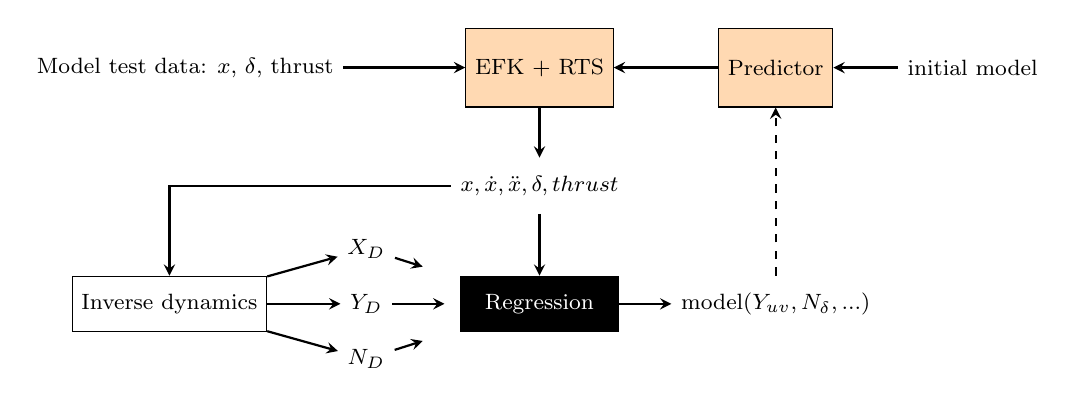
\begin{tikzpicture}[node distance=1.5cm]
    %\draw (0,0) rectangle (10,10); %create a bounding box to reserve space
    \node (data) [io] {\footnotesize Model test data: $x$, $\delta$, thrust};
    
    \node (EKF) [process, right of=data, xshift=3.0cm] {\footnotesize EFK + RTS};
    \node (predictor) [process, right of=EKF, xshift=1.5cm]{\footnotesize Predictor};
    \node (VMM) [io, right of=predictor, xshift=1.0cm] {\footnotesize initial model};
    
    \node (data_clean) [io, below of=EKF] {\footnotesize \(x,\dot{x},\ddot{x}, \delta, thrust\)};
    
    \node (black-box) [black-box, below of=data_clean] {\footnotesize Regression};
    
    \node (X_D) [io, left of=black-box, xshift=-0.70cm, yshift=0.7cm]{\footnotesize \(X_D\)};
    \node (Y_D) [io, left of=black-box, xshift=-0.70cm, yshift=0cm]{\footnotesize \(Y_D\)};
    \node (N_D) [io, left of=black-box, xshift=-0.70cm, yshift=-0.7cm]{\footnotesize \(N_D\)};
    
    \node (white-box) [white-box, left of=Y_D, xshift=-1.00cm] {\footnotesize Inverse dynamics};
    
    
    %
    %
    \node (coefficients) [io, right of=black-box, xshift=1.5cm] {\footnotesize model$\left(Y_{uv},N_{\delta},...\right)$};
    
    \draw [arrow] (data) -- (EKF);
    \draw [arrow] (predictor) -- (EKF);
    \draw [arrow] (VMM) -- (predictor);
    \draw [arrow] (EKF) -- (data_clean);
    
    \draw [arrow] (data_clean) -| (white-box);
    \draw [arrow] (data_clean) -- (black-box);
    
    \draw [arrow] (white-box) -- (X_D);
    \draw [arrow] (white-box) -- (Y_D);
    \draw [arrow] (white-box) -- (N_D);
    
    \draw [arrow, shorten >=0.5cm] (X_D) -- (black-box);
    \draw [arrow, shorten >=0.2cm] (Y_D)  -- (black-box);
    \draw [arrow, shorten >=0.5cm] (N_D)  -- (black-box);
    
    
    \draw [arrow] (black-box)  -- (coefficients);
    \draw [arrow, dashed] (coefficients)  -- (predictor);
    
    \end{tikzpicture}
    \caption{Method to estimate the manoeuvring model hydrodynamic derivatives.}
    \label{fig:greyvmm}
\end{figure}

\noindent Using semi-empirical formulas (\autoref{app:initial_estimates}) for the initially estimated manoeuvring model adds prior knowledge about the ship dynamics to the regression. An example, with simulation results from the steps in the iteration, is presented in \hyperref[\detokenize{01.01_method:iterations}]{\autoref{\detokenize{01.01_method:iterations}}}.


\begin{figure}[H]
    \centering
    \includegraphics[width=\textwidth]{kappa/images/0.pdf}
    \caption{Simulation with: initial model and first and second iteration of the parameter estimation method.}
    \label{\detokenize{01.01_method:iterations}}
\end{figure}
\section{Generalization of models} \label{sec:generalization}
Generalization refers to a model's ability to perform well on new, unseen data, rather than just the data it was trained on. This is crucial because the ultimate goal of a model is to make accurate predictions on real-world data, not just the training dataset.

For data driven models overfitting can be a problem. The model learns the training data too well, including noise and outliers so that it performs poorly on new data. The opposite, underfitting the data can also be a problem. The model is too simple to capture the underlying patterns in the data, leading to poor performance on both training and new data.  

The bias–variance tradeoff is a fundamental concept in understanding generalization. A model with high bias (underfitting) makes strong assumptions about the data, while a model with high variance (overfitting) is too sensitive to the training data. The goal is to find a balance between bias and variance to achieve good generalization

Cross validation is one way to prevent overfitting, which is further explained in the next section.

\section{Cross validation}
\label{sec:cross_validation}
 The aim of developing a manoeuvring model with parameter estimation is to develop a model that can generalize outside the known data. The method presented in this thesis is assessed with the hold-out evaluation \cite{sammutHoldoutEvaluation2017}. The data in this evaluation is divided into three sets: the training set, the validation set, and the test set as seen in \autoref{fig:model_development_process}.
The purpose of the training set is to train all the candidate models using the proposed parameter estimation method. The validation set is used to select the most effective candidate model. The training and validation sets are joined to train the selected model as the final model. The final model is used for predicting the test set, which is used to evaluate the accuracy of the model. These three sets are not divided randomly;  they are divided to assess the model’s extrapolation ability. The data sets are therefore split to have the smallest yaw rates, drift-angles, and rudder-angles in the training set; the medium values in the validation set; and the largest values in the test set.
Examples of this can be seen for the two test cases in this thesis in \autoref{fig:kvlcc2_datasets} and  \autoref{fig:wpcc_datasets} in the next chapter.
\begin{figure}[H]
\centering
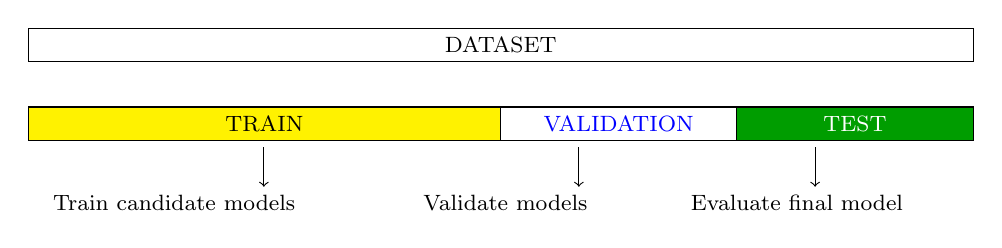
\begin{tikzpicture}

\node (dataset)[rectangle,
    anchor=west,
    draw,
    text = black,
    minimum width=12cm,
    fill = white] at (0, 0) {\footnotesize DATASET};

\node (train)[rectangle,
    draw,
    anchor=west,
    text = black,
    minimum width=6cm,
    fill = yellow] at (0, -1cm) {\footnotesize TRAIN};

\node (validation)[rectangle,
    draw,
    anchor=west,
    text = blue,
    minimum width=3cm,
    fill = white] at (6cm, -1cm) {\footnotesize VALIDATION};

\node (test)[rectangle,
    draw,
    anchor=west,
    text = white,
    minimum width=3cm,
    fill = black!15!green!255] at (9cm, -1cm){\footnotesize TEST};
    
\node (train_multiple)[rectangle,
    draw,
    anchor=west,
    text = black,
    draw = none,
    fill = none] at (0.2cm, -2cm){\footnotesize Train candidate models};
    
\node (validate_models)[rectangle,
    draw,
    anchor=west,
    text = black,
    draw = none,
    fill = none] at (4.9cm, -2cm){\footnotesize Validate models};
    
\node (evaluate_models)[rectangle,
    draw,
    anchor=west,
    text = black,
    draw = none,
    fill = none] at (8.3cm, -2cm) {\footnotesize Evaluate final model};

\draw[->] (3,-1.3) -- (3,-1.8);
\draw[->] (7,-1.3) -- (7,-1.8);
\draw[->] (10,-1.3) -- (10,-1.8);
\end{tikzpicture}
\caption{Model development process with hold-out evaluation.}
\label{fig:model_development_process}
\end{figure}
\section{Test cases} \label{sec:test_cases}
Two test cases have been studied in this thesis. The wPCC test case is a ship that was designed for wind-assisted propulsion system (WAPS) and can alter between a fully sailing mode, and a fully motoring mode, and in between. 
However, this thesis only considers the motoring mode. Because of the WAPS, the wPCC design differs slightly from conventional motoring cargo ship designs. The wPCC has two very large rudders, two to three times larger than needed for a conventional ship. The ship also has fins at the bilge to generate extra lift while sailing, as shown on the scale model in \autoref{fig:wPCC}.
\autoref{tab:main_particulars} shows the main particulars of the scale model. 
\begin{figure}[h]
    \centering
    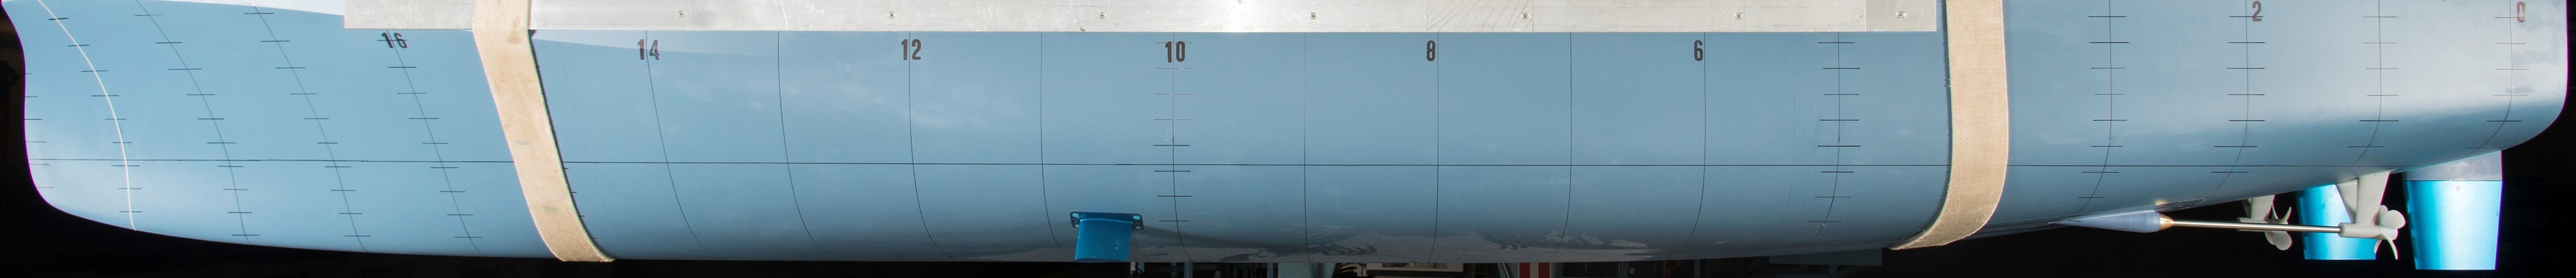
\includegraphics[width=\columnwidth]{figures/5m2.jpg}
    \caption{Scale model of the wPCC used in the model tests. Copyright RISE.}
    \label{fig:wPCC}
\end{figure}

The Optiwse test case is an ordinary VLCC tanker but with a larger rudder size adopted for WAPS as shown in the scale model in  \autoref{fig:optiwise}. \autoref{tab:main_particulars} shows the main particulars of the scale model. 
\begin{figure}[h]
    \centering
    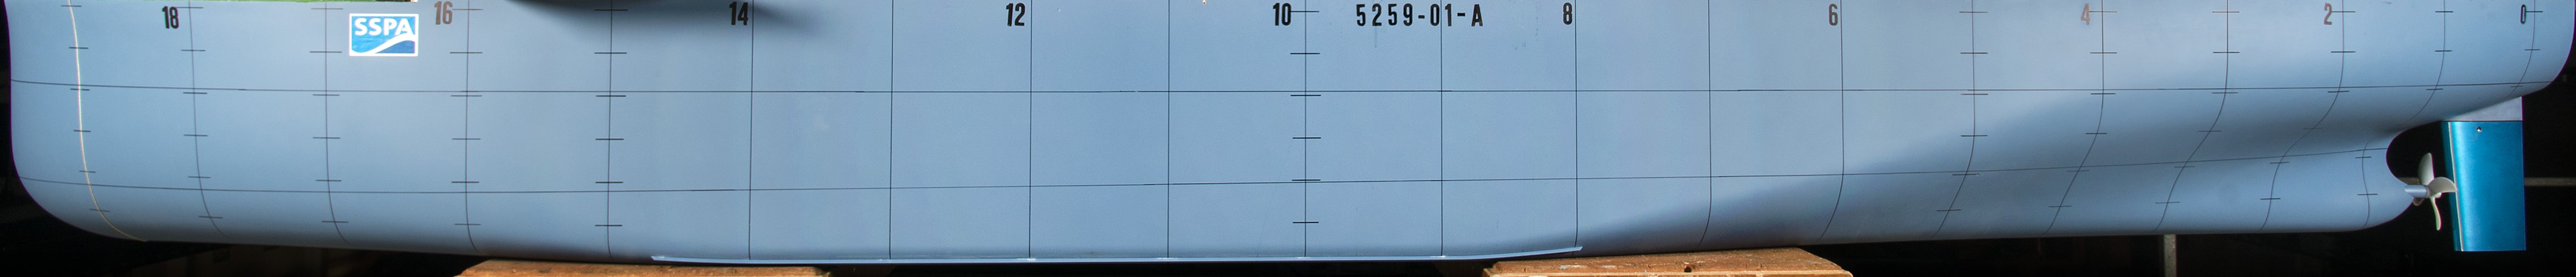
\includegraphics[width=\columnwidth]{figures/optiwise.jpg}
    \caption{Scale model of the Optiwise used in the model tests. Copyright RISE.}
    \label{fig:optiwise}
\end{figure}
\begin{table}[h]
    \centering
    \caption{Main particulars of the test case scale models.}
    \label{tab:main_particulars}
    \pgfplotstabletypeset[col sep=comma, column type=r, columns={Parameter,Unit, wPCC, Optiwise, Description},
        columns/Parameter/.style={column type=l,string type},
        columns/Unit/.style={column type=l,string type, column name=~},
        columns/wPCC/.style={column type=r},
        columns/Optiwise/.style={column type=r},
        columns/Description/.style={column type=l,string type},
        every head row/.style={before row=\hline,after row=\hline},
        every last row/.style={after row=\hline}
    ]{tables/test_cases.main_particulars.csv}
\end{table}


%%%%%%%%%%%%%%%%%%%%%%%%%%%%%%%
%%%%%%%%%%%%%%%%%%%%%%%%%%%%%%%
\chapter{Summary and discussions of appended papers}\label{ch:results}
\noindent This chapter presents a summary of the appended papers, which includes research activities and a selection of the most relevant results, also see \autoref{tab:objectives} in \autoref{sec:motivation} for a summary of how these papers connect to the research objectives of this thesis.
%Section Comments: "Second generation intact stability criteria" seems more commonly used. It would help to specify a specific time period instead of saying "a long time."
\section{Summary of Paper \ref{pap:rolldamping}}
\subsection*{"\nameref{pap:rolldamping}"}
\subsection*{Scope and motivations}
The first step in this research project was to limit the system identification of the ship dynamics to only one degree of freedom. An accurate modeling of the roll motion is crucial, where 

\textcite{france_investigation_2001} demonstrated that the APL China casualty in 1998, where a post-Panamax C11 class container ship lost almost a third of its containers, was most likely caused by head sea parametric rolling.

was investigated in Paper \ref{pap:rolldamping} 

\subsection*{Results and concluding remarks}


System identification of ship roll motion, which includes roll damping and stiffness, is developed in Paper \ref{pap:rolldamping}. Parametric roll was observed by \textcite{froude_rolling_1861} and has been a focus of the marine research community since the early 1950s \parencite{galeazzi_early_2013}; it has received even more attention since \textcite{france_investigation_2001} demonstrated that the APL China casualty in 1998, where a post-Panamax C11 class container ship lost almost a third of its containers, was most likely caused by head sea parametric rolling. The damping of roll motion plays an important role in these phenomena. Previous literature demonstrates that the relatively small difference in the roll damping prediction obtained with small method variation may contribute to the difference between severe roll angles and much less noticeable motions \cite{soder_ikeda_2019}.

The objective of Paper \ref{pap:rolldamping} was to improve the roll damping predictions for modern ships. The roll damping was studied using time series data from 250 (see \autoref{fig:ship_types}) roll decay tests (see \autoref{sec:roll}) assembled by the Maritime Dynamics Laboratory at RISE SSPA Maritime center. The work was divided into the following sub tasks (also summarized in \autoref{fig:paper1_overview}): 
\vspace{5pt}
\begin{itemize}
    \setlength\itemsep{5pt}
    \item Find the mathematical model that is the best representation of the roll motion.
    \item Identify the parameters in this model for all the tests.
    \item Compare the identified parameters with state of art predictions.
    \item Develop a generic roll damping model for all ships using the identified parameters.
    \begin{itemize}
        \item Grey-box model
        \item Black-box model
    \end{itemize}
\end{itemize}
\vspace{5pt}
\begin{figure}[!htb]
    \centering
    \includegraphics[width=0.6\columnwidth]{kappa/images/ship_types.eps}
    \caption{Number of tests per ship type.}
    \label{fig:ship_types}
\end{figure}
\begin{figure}[!htb]
    \centering
\begin{tikzpicture}[node distance=3cm]
\node (data_collection) at (0,0) {Data collection:};
\node (roll_decay_DB) [database,label=below:Roll decay DB, right of=data_collection, xshift=-0.5cm]{};
\node (PIT) [process, right of=roll_decay_DB, xshift=0.5cm] {PIT};
\node (damping_DB) [database, label=below:Damping DB, right of=PIT, xshift=0cm] {};
\path (roll_decay_DB) -- node(time_series)[xshift=3.0cm]{Time series} -- (PIT);
\draw [arrow] (roll_decay_DB) -- (time_series) -- (PIT);
\path (PIT) -- node(B){B} (damping_DB);
\draw [arrow] (PIT) -- (B) -- (damping_DB);

\node (comparison)[below of=data_collection, yshift=0.5cm]{Comparison:};
%plot:
\node (origo)[right of=comparison, xshift=-0.5cm, yshift=-1cm];
\node(y)[above of=origo, yshift=-1cm]{Simplified ikeda};
\node(x)[right of=origo, xshift=-1cm]{Damping DB};
\draw[->](origo) -- (y);
\draw[->](origo) -- (x);
\draw node[anchor=south, right of=origo, xshift=-3cm, yshift=0cm] {\textbullet};
\draw node[anchor=south, right of=origo, xshift=-2.5cm, yshift=0.6cm] {\textbullet};
\draw node[anchor=south, right of=origo, xshift=-2cm, yshift=1cm] {\textbullet};
\draw node[anchor=south, right of=origo, xshift=-2cm, yshift=1.2cm] {\textbullet};
\draw node[anchor=south, right of=origo, xshift=-1.5cm, yshift=1.7cm] {\textbullet};
\draw node[anchor=south, right of=origo, xshift=-1.5cm, yshift=1.3cm] {\textbullet};
\draw node[anchor=south, right of=origo, xshift=-1cm, yshift=2cm] {\textbullet};

\node (regressions)[below of=comparison, yshift=-0.5cm]{Regressions:};
\node (damping_DB2) [database,label=below:Damping DB, right of=regressions, xshift=-0.5cm]{};
\node (grey_box) [grey-box, right of=damping_DB2, xshift=0.5cm, yshift=1.5cm] {Grey-box};
\node (black_box) [black-box, below of=grey_box, yshift=1.5cm] {Black-box};
\draw [arrow] (damping_DB2) |- (grey_box);
\draw [arrow] (damping_DB2) -- (black_box);
\end{tikzpicture}
    \caption{Overview of the work conducted for Paper \ref{pap:rolldamping}.}
    \label{fig:paper1_overview}
\end{figure}
System identification on the time series from the roll decay database was performed with the linear (\autoref{eq:roll_decay_equation_himeno_linear}), quadratic (\autoref{eq:roll_decay_equation_himeno_quadratic_b}), and cubic models (\autoref{eq:roll_decay_equation_cubic}). Estimated roll damping parameters were used to build a roll damping database. The database could be compared to corresponding predictions with the simplified Ikeda's method \cite{kawahara_simple_2011}, which is the state of art prediction for ship roll damping.
The generic roll damping model was developed as a grey-box model and a black-box model.
\subsection{Best mathematical model for the roll motion}
System identification on the linear, quadratic, and cubic models was conducted using both the \say{integration approach} (\autoref{sec:integration_approach}) and the \say{derivation approach} (\autoref{sec:derivation_approach}) where the best parameter estimations were obtained using the ``integration approach''.
Results from the simulations with the identified models (from one of the roll-decay tests) are presented in \autoref{fig:roll_decay_compare}. The cubic and quadratic models reproduce the model test well, and the linear model is too simple to provide an accurate representation for both smaller and larger roll angles. The amplitude decrement $\phi_a$ and roll damping $B$ for each oscillation can be visualized, as seen in \autoref{fig:roll_decay}.
\begin{figure}[h!]
    \centering
    \includegraphics[width=\linewidth]{kappa/images/roll_decay_model_compare.pdf}
    \caption{Roll decay estimation with identified cubic, quadratic, and linear models.}
    \label{fig:roll_decay_compare}
\end{figure}
\begin{figure}[h!]
    \begin{subfigure}[b]{0.45\textwidth}
        \centering
        \includegraphics[width=0.9\linewidth]{kappa/images/roll_decay_amplitude.pdf}
        \caption{Amplitude decrements.}
        \label{fig:roll_decay_amplitude}
    \end{subfigure}
        ~ %add desired spacing between images, e. g. ~, \quad, \qquad, \hfill etc. 
      %(or a blank line to force the subfigure onto a new line)
    \begin{subfigure}[b]{0.45\textwidth}
        \centering
        \includegraphics[width=0.9\linewidth]{kappa/images//roll_decay_damping.pdf}
        \caption{Dampings.}
        \label{fig:roll_decay_damping}
    \end{subfigure}
    \caption{Roll decay model test, linear-, quadratic- and cubic-model.}
    \label{fig:roll_decay}
\end{figure}
The goodness of fit for the linear, quadratic, and cubic models can be expressed using the coefficient of determination:
\begin{equation} \label{eq:R2}
%R^2=1-\frac{SS_{res}}{SS_{tot}}
R^2=1-\frac{\sum\limit_{i=1}^{n}(\phi_{i}-\hat{\phi}_i)^2}{\sum\limit_{i=1}^{n}(\phi_i-\bar \phi)^2}
\end{equation}
where $\phi_i$ is the model test roll angle at time step $i$, $\bar \phi$ is the mean roll angle from the model test, and $\hat{\phi}_i$ is the predicted roll angle (with the linear, quadratic, or cubic model). The average goodness of fit $R^2$ was 0.995 for the cubic model, 0.993 for the quadratic model, and 0.986 for the linear model. These values indicate that the quadratic model is almost as useful as the cubic model for describing the roll motion. The quadratic model, with fewer parameters than the cubic model, is expected to have a higher level of generalization at the same accuracy and is therefore selected as the best mathematical model for the roll motion. 

\subsection{Comparison with Ikeda's method}
The hydrodynamic analysis requires the ship's exact hull geometry. Building the geometry model and performing the strip-theory based hydrodynamic analysis are time-consuming. A ship's hull geometry is not always available for such purposes. A simplified Ikeda's method (SI-method) proposed by \textcite{kawahara_simple_2011} is used in Paper \ref{pap:rolldamping} to calculate all the damping components, which include the eddy component $B_E$ and the wave component $B_W$. The semi-empirical formulas describe four of the five roll damping components at motion frequency $\omega$ for a given roll amplitude $\phi_a$ at zero ship speed. A speed dependency was introduced by adding a fifth damping term $B_L$ and a speed correction to $B_W$ and $B_E$, as described in \textcite{ikeda_velocity_1979}, giving a function: 
\input{equations/simplified_ikeda_equation}

\noindent The formulas within $f$ can be expressed as \textcite{ikeda_velocity_1979, kawahara_simple_2011} with the implementation in \textcite{alexandersson_rolldecay-estimators_2022}.
It should be noted that this method is only efficient for the estimation of the roll damping of ships within the boundaries \parencite{kawahara_simple_2011}:
\begin{equation}
    \label{eq:SI_limits}
     \left\{
     \begin{array}{ll}
    0.5 \leq C_b \leq 0.85,\hspace{0.5cm} 
    0 \leq \hat{\omega} \leq 1.0,
    \hspace{0.5cm}
    0.9 \leq A_0 \leq 0.99,\\
    2.5\leq Beam/T \leq 4.5, \hspace{1cm}
    0.01 \leq BK_B/Beam \leq 0.06, \\
        -1.5 \leq OG/T \leq 0.2,
     \hspace{1cm}
    0.05 \leq BK_L/L_{PP} \leq 0.4.
    \end{array}
    \right.
\end{equation}

\noindent The total roll damping is predicted as the sum (\autoref{eq:ikeda}) of the damping contributions (\autoref{eq:simplified_ikeda_equation}). This damping can be compared with the linearized equivalent damping $B_e$, which is calculated for a certain roll angle $\phi_a$ with the identified roll damping parameters $B_1$ and $B_2$ \cite{himeno_prediction_1981},
\input{equations/B_e_equation}

\noindent The $B_e$ non-dimensional form of the coefficient can be used according to \textcite{himeno_prediction_1981}. The non-dimensional equivalent for the linear damping coefficient is $\hat{B_e}$. This form is more convenient when comparing roll damping for different ships,
\begin{equation} \label{eq:be_eqvalent}
    \hat{B_e} = \frac{B_e}{\rho \bigtriangledown Beam^2} \sqrt{\frac{Beam}{2g}},
\end{equation}
\noindent where $\rho$, $\bigtriangledown$, and $Beam$ stand for fluid density, displacement volume, and breadth of a ship, respectively. Prediction error plots of $\hat{B_e}$ from the simplified Ikeda's method and identified damping from the model tests are presented in \autoref{fig:si_model_within}. In this figure, a comparison of predictions with roll amplitudes in the range of 0 to 10 degrees is displayed for all ships with no limits and for ships within the limits of the method (\autoref{eq:SI_limits}). The $R^2$ values of the predictions are displayed in \autoref{tab:si_validation}. There is reasonable agreement between the predicted roll damping and model tests for ships within the limits. There is very poor agreement for ships outside the limits. It should be noted that most of the points are outside the limits of the method.

\begin{figure}[h!]
\centering
    \begin{subfigure}[b]{0.45\textwidth}
    
        \centering
        \includegraphics[width=\textwidth]{kappa/images/si_model_within.pdf}
        %\vspace{-0.5cm}
        \caption{The simplified Ikeda's method within and outside its limits.}
        \label{fig:si_model_within}
    \end{subfigure}
    \hfill
    \begin{subfigure}[b]{0.45\textwidth}
        \centering
        \includegraphics[width=\textwidth]{kappa/images/component_residual.pdf}
        \vspace{-0.2cm}
        \caption{Residuals vs. components.}
        \label{fig:component_residual}
        \vspace{0.3cm}
    \end{subfigure}
    \hfill
    \begin{subfigure}[b]{0.45\textwidth}
        \centering
        \includegraphics[width=\textwidth]{kappa/images/si_ikeda_model.pdf}
        \caption{Comparison of simplified and original Ikeda's method and model tests.}
        \label{fig:si_ikeda_model}
    \end{subfigure}

    \caption{Prediction error plots.}
\end{figure}
\input{equations/si_validation}
\noindent The largest contribution to the error in the predictions comes from the wave damping $B_W$, as seen in \autoref{fig:component_residual}. A comparison of the simplified Ikeda's method and the original Ikeda's method was carried out in Paper \ref{pap:rolldamping}; the comparison was used to determine whether the observed deviations are the result of extrapolation or inherent to the original method. In Ikeda's method, more extensive knowledge of the ship hull geometry is needed in order for $B_W$ to be calculated with a strip method and $B_E$ to be calculated with sectional Lewis coefficients. It was possible to collect the required hull inputs for 15 ships in the database. These ships were used in 50 of the reference roll decay tests; all but one of the tests exceed the limits. Ikeda's method has much more agreement for these exceeding model tests according to \autoref{fig:si_ikeda_model} and the calculated $R^2$ in Table \ref{tab:si_ikeda_validation}.

\input{equations/si_ikeda_validation}
\subsection{Generic roll damping model}
\label{sec:genericrolldampingmodel}
A serial grey-box model for ship roll damping (see \autoref{fig:greyrolldamping}) is also developed in Paper \ref{pap:rolldamping}. 
This is expanding the system identification by not only focusing on one ship, but all modern ships. 
The simplified Ikeda's method \cite{kawahara_simple_2011} is used as the white-box model, which is combined with the following black-box correction model.

\begin{figure}[H]
    
    \centering
    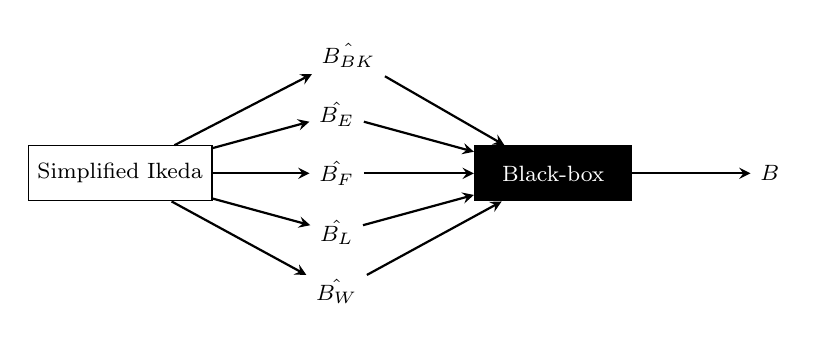
\begin{tikzpicture}[node distance=2cm]
    \node (white-box) [white-box] {\footnotesize Simplified Ikeda};
    \node (B_BK) [io, right of=white-box, xshift=0.90cm, yshift=1.5cm] {\footnotesize $\hat{B_{BK}}$};
    \node (B_E) [io, right of=white-box, xshift=0.75cm, yshift=0.75cm] {\footnotesize $\hat{B_{E}}$};
    \node (B_F) [io, right of=white-box, xshift=0.75cm, yshift=0cm] {\footnotesize $\hat{B_{F}}$};
    \node (B_L) [io, right of=white-box, xshift=0.75cm, yshift=-0.75cm] {\footnotesize $\hat{B_{L}}$};
    \node (B_W) [io, right of=white-box, xshift=0.75cm, yshift=-1.5cm] {\footnotesize $\hat{B_{W}}$};
    
    
    \node (black-box) [black-box, right of=B_F, xshift=0.75cm] {\footnotesize Black-box};
    \draw [arrow] (white-box) -- (B_BK);
    \draw [arrow] (white-box) -- (B_E);
    \draw [arrow] (white-box) -- (B_F);
    \draw [arrow] (white-box) -- (B_L);
    \draw [arrow] (white-box) -- (B_W);
    
    \draw [arrow] (B_BK) -- (black-box);
    \draw [arrow] (B_E)  -- (black-box);
    \draw [arrow] (B_F)  -- (black-box);
    \draw [arrow] (B_L)  -- (black-box);
    \draw [arrow] (B_W)  -- (black-box);
    
    
    \node (B) [io, right of=black-box, xshift=0.75cm, yshift=0cm] {\footnotesize $B$};
    \draw [arrow] (black-box)  -- (B);
    
    \end{tikzpicture}
    \caption{Grey-box model to predict roll damping.}
    \label{fig:greyrolldamping}
\end{figure}

\noindent The roll damping data set, obtained from the roll motion investigation, is intended to train the black-box component of the grey-box model. The black-box correction model of the output components from the simplified Ikeda's method is displayed in (\autoref{eq:polynom_correction}),
\input{equations/polynom_correction}

\noindent Major corrections to the skin friction damping $\hat{B_F}$ and wave damping $\hat{B_W}$ are included in this expression. The corrections are included because the simplified Ikeda's method is not very accurate for this dataset; most of the ships in the dataset exceeded the limits of the method. A pure black-box model is also developed in Paper \ref{pap:rolldamping} (see \autoref{eq:polynom_complex}),
\input{equations/polynom_complex}
\noindent where non-dimensional frequency $\hat{\omega_0}$ is calculated with \autoref{eq:omega0_hat_equation} \cite{himeno_prediction_1981},
\input{equations/omega0_hat_equation}
Over-fitting data is a concern when constructing a regression model from a data set. Including too many parameters or allowing the order of the model to be too high would provide a very accurate representation of the present roll damping data. However, such a representation would be accompanied by major extrapolation errors when the model is used for other data. The generalization of the model can be assessed with a hold-out evaluation by using K-fold cross validation \cite{mosteller_handbook_1968} (\autoref{fig:k-fold}).\input{kappa/fig_k-fold} The data has been divided into five smaller sets (folds). Four of the folds are used to train the model, and the fifth fold is used for testing (validation). Validation consists of calculating the coefficient of determination $R^2$ for the fitted model. Validation is completed for all five possible train-test combinations. 
The folds are randomly constructed with the restriction that all data for a particular ship must be in the same fold. Five folds are randomly generated 20 times, which gives 100 values of $R^2$ from the train-test-procedure for each model. The mean values and standard deviation of these 100 values of $R^2$ are displayed in Table \ref{tab:crossvalidation}. The mean and standard deviation of $R^2$ simplified Ikeda's method in this table were calculated directly instead of using cross validation because they do not rely on the SSPA data.
\input{equations/cross_validation}
\clearpage
\section{Summary of Paper \ref{pap:ikeda}}
\subsection*{"\nameref{pap:ikeda}"}
\subsection*{Scope and motivations}
An explicit semi-empirical formula was proposed in Paper \ref{pap:rolldamping}, based on the simplified Ikeda's method \cite{kawaharaSimplePredictionFormula2011}. This is an alternative with very low computational cost. However, it was also found to have poor accuracy, especially for modern ship designs. 
Paper \ref{pap:ikeda} proposed a new hybrid method, as a solution to this problem, where the viscous roll damping from Ikeda’s semi-empirical method was injected into an existing 3D unsteady fully nonlinear potential flow (FNPF) method \cite{kjellbergFullyNonlinearUnsteady2013}.

\subsection*{Results and concluding remarks}
The viscous roll damping was calculated with Ikeda's method \cite{ikedaComponentsRollDamping1978} for the KVLCC2 test case. Error in the calculation of the $C_r$ coefficient to obtain the eddy damping at zero speed was encountered, which was found to originate from a regression formula from experiments conducted by \textcite{ikedaEddyMakingComponent1978} on a number of two-dimensional cylinders with various sections. A new regression was instead proposed, using a decision tree model.
Fig.\ref{fig:ikeda_sections} shows $C_r$ from the experiments and corresponding predictions with Ikeda's method and the decision tree. The capital letters refer to cylinder sections from the experiments
\cite{ikedaEddyMakingComponent1978}.
\begin{figure}[h]
\center
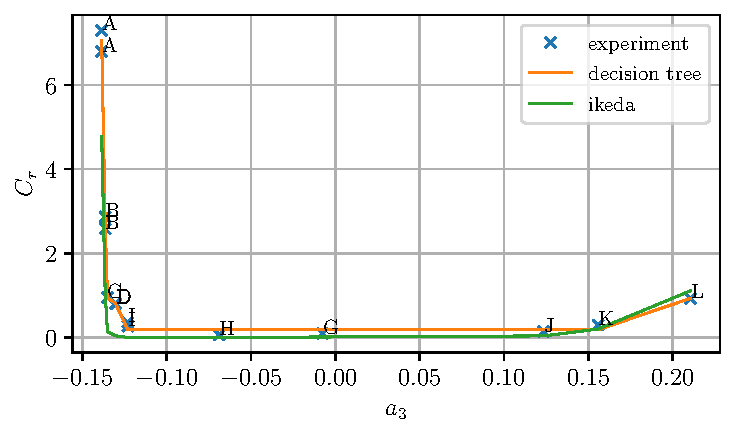
\includegraphics[width=\textwidth]{figures/ikeda_sections.pdf}
\vspace{-0.4cm}
\caption{$C_r$ for cylinder sections from experiments and predicted with Ikeda's method and the decision tree model.}
\label{fig:ikeda_sections}
\end{figure}
\FloatBarrier

The total predicted roll damping was reasonably in good agreement with the damping of the model tests at zero speed (\autoref{fig:hybrid_0}) and very well in agreement at speed (\autoref{fig:hybrid_speed}).
\begin{figure}[h]
\begin{center}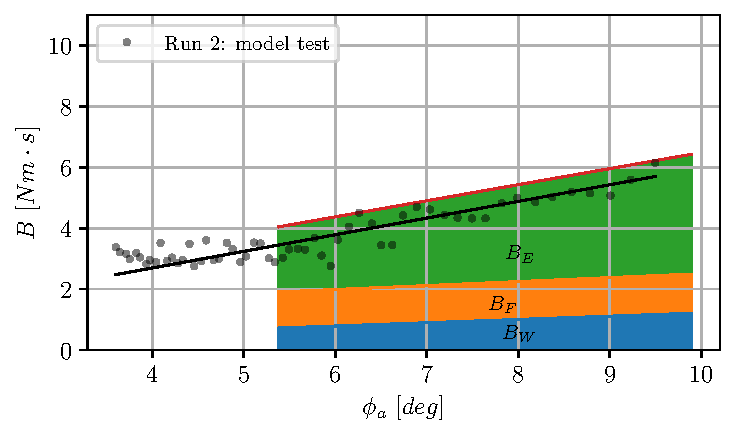
\includegraphics[width=\textwidth]{figures/hybrid_0.pdf}\end{center}
%\vspace{-0.4cm}
\caption{Roll damping from hybrid method ($F_n = 0$) for KVLCC2.}
\label{fig:hybrid_0}
\end{figure}
\begin{figure}[h]
\begin{center}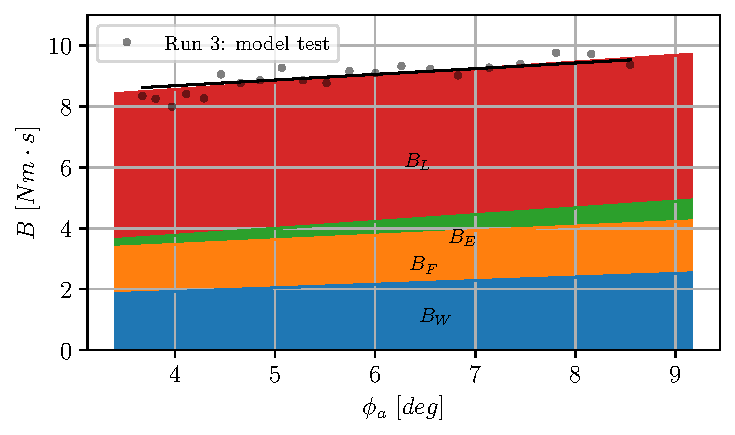
\includegraphics[width=\textwidth]{figures/hybrid_speed.pdf}\end{center}
%\vspace{-0.4cm}
\caption{Roll damping from hybrid method ($F_n = 0.14$) for KVLCC2.}
\label{fig:hybrid_speed}
\end{figure}
Roll decay simulations with damping from the hybrid method were conducted. Results from these simulations were compared with the model tests at zero speed (\autoref{fig:hybrid_0_time}) and at speed (\autoref{fig:hybrid_speed_time}). The time series from the corresponding FNPF
simulations have also been added to these plots to show how much the injection of semi-empirical viscous damping can improve the accuracy of these simulations.

Paper \ref{pap:ikeda} concluded that Ikeda's method offers an effective semi-empirical approach for predicting viscous roll damping. When combined with modern potential flow codes like FNPF, it enables highly accurate predictions of ship roll motion 
\begin{figure}[h]
\center
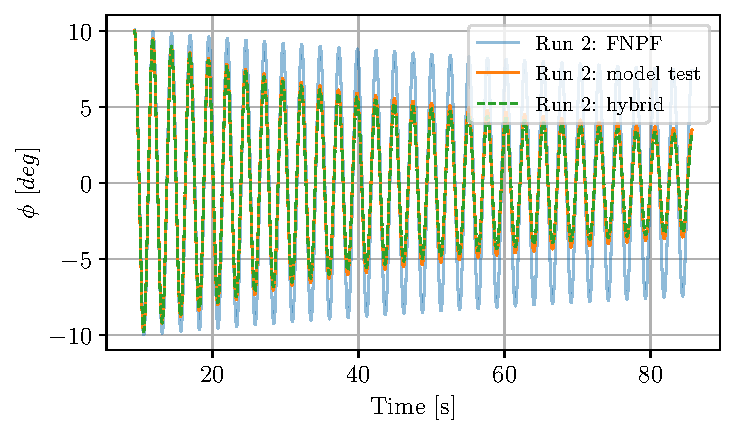
\includegraphics[width=\textwidth]{figures/hybrid_0_time.pdf}
%\vspace{-0.7cm}
\caption{Roll decay ($F_n=0$) for KVLCC2.}
\label{fig:hybrid_0_time}
\end{figure}
\begin{figure}[h]
\center
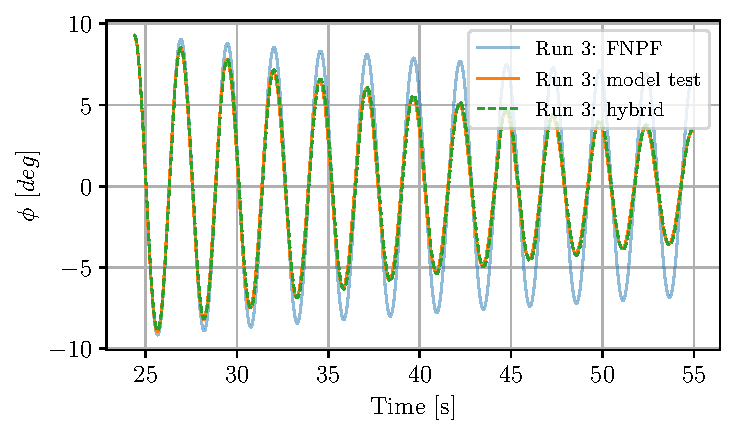
\includegraphics[width=\textwidth]{figures/hybrid_speed_time.pdf}
%\vspace{-0.7cm}
\caption{Roll decay ($F_n=0.14$) for KVLCC2.}
\label{fig:hybrid_speed_time}
\end{figure}
\section{Summary of Paper \ref{pap:pit}}
\subsection*{"\nameref{pap:pit}"}
\subsection*{Scope and motivations}
In order to expand the modeling complexity and uncertainty from Paper \ref{pap:rolldamping}, system identification of manoeuvring by adding the the surge, sway, and yaw degrees of freedom was studied in Paper \ref{pap:pit}. 
The objective was to find parametric model structures with good generalization and to develop parameter identification techniques from FRMT data.

The dynamics were assumed to be described by an Abkowitz or truncated Abkowitz model. 
The system identification method proposed in Paper \ref{pap:pit} was validated on two case study ships: the wPCC and the KVLCC2 (\autoref{fig:kvlcc2_hsva}). The parameters were identified with recursive inverse dynamics regression (see \autoref{sec:RIDR}).
The identification was carried out with cross validation using hold-out evaluation \cite{sammutHoldoutEvaluation2017}.
The data in this evaluation were divided into three sets: the training set, the validation set and the test set as seen in \autoref{fig:model_development_process}.
The purpose of the training set was to train all the candidate models using the proposed parameter estimation method. The validation set was used to select the most effective candidate model. The training and validation sets were joined to train the selected model as the final model. The final model was used for predicting the test set, which was used to evaluate the accuracy of the model. These three sets were not divided randomly;  they were divided to assess the model’s extrapolation ability. The data sets were therefore split to have the smallest yaw rates, drift-angles, and rudder-angles in the training set; the medium values in the validation set; and the largest values in the test set.
Examples of this can be seen for the two test cases in \autoref{fig:wpcc_datasets} and \autoref{fig:kvlcc2_datasets}.
%\begin{figure}[h!]
%\centering
%\includegraphics[width=0.5\linewidth]{kappa/images/wpcc_mdl.png}
%\caption{wPCC tested at SSPA Maritime center. Copyright 2020 by RISE.}
%\label{fig:wpcc-mdl}
%\end{figure}
\begin{figure}[h!]
    \centering
    \begin{subfigure}[b]{0.45\textwidth}
    \centering
    \includegraphics[height=3cm]{kappa/images/kvlcc2_front.png}
    \end{subfigure}
    ~
     \begin{subfigure}[b]{0.45\textwidth}
     \centering
     \includegraphics[height=3cm]{kappa/images/kvlcc2_aft.png}
     \end{subfigure}
+    \caption{Ship model used in HSVA and MARIN model tests. Copyright HSVA.}
    \label{fig:kvlcc2_hsva}
\end{figure}
\begin{figure}[H]
\centering
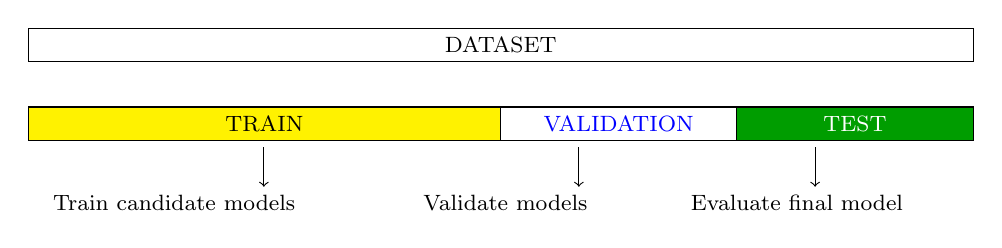
\begin{tikzpicture}

\node (dataset)[rectangle,
    anchor=west,
    draw,
    text = black,
    minimum width=12cm,
    fill = white] at (0, 0) {\footnotesize DATASET};

\node (train)[rectangle,
    draw,
    anchor=west,
    text = black,
    minimum width=6cm,
    fill = yellow] at (0, -1cm) {\footnotesize TRAIN};

\node (validation)[rectangle,
    draw,
    anchor=west,
    text = blue,
    minimum width=3cm,
    fill = white] at (6cm, -1cm) {\footnotesize VALIDATION};

\node (test)[rectangle,
    draw,
    anchor=west,
    text = white,
    minimum width=3cm,
    fill = black!15!green!255] at (9cm, -1cm){\footnotesize TEST};
    
\node (train_multiple)[rectangle,
    draw,
    anchor=west,
    text = black,
    draw = none,
    fill = none] at (0.2cm, -2cm){\footnotesize Train candidate models};
    
\node (validate_models)[rectangle,
    draw,
    anchor=west,
    text = black,
    draw = none,
    fill = none] at (4.9cm, -2cm){\footnotesize Validate models};
    
\node (evaluate_models)[rectangle,
    draw,
    anchor=west,
    text = black,
    draw = none,
    fill = none] at (8.3cm, -2cm) {\footnotesize Evaluate final model};

\draw[->] (3,-1.3) -- (3,-1.8);
\draw[->] (7,-1.3) -- (7,-1.8);
\draw[->] (10,-1.3) -- (10,-1.8);
\end{tikzpicture}
\caption{Model development process with hold-out evaluation.}
\label{fig:model_development_process}
\end{figure}
\begin{figure}[h!]
\centering
\includegraphics[width= 1.0\linewidth]{kappa/images/3.pdf}
\caption{wPCC training, validation and testing datasets.}
\label{fig:wpcc_datasets}
\end{figure}
\begin{figure}[h!]
\centering
\includegraphics[width=1.0\textwidth]{kappa/images/4.pdf}
\caption{KVLCC2 training, validation and testing datasets.}\label{fig:kvlcc2_datasets}
\end{figure}

\subsection*{Results and concluding remarks}
\autoref{fig:validation-forces} shows predictions of the wPCC validation set with the identified models. AVMM is a full Abkowitz model and MAVMM is a truncated Abkowitz model where model structure selection has been applied. The AVMM model over-predicted the forces by far. 
This over-prediction was  explained by the high multicollinearity of the AVMM model structure for the wPCC data as shown in \autoref{fig:ncorr}  where the absolute correlation coefficient between the features in the wPCC yaw moment regression is presented.
Therefore, simulations of the validation cases were only possible using the MAVMM. 
The MAVMM model was retrained on the joined test and validation data set to obtain the final prediction model which was used to predict the turning circle test data set as shown in \autoref{fig:track-plot-testing-sim}. Advance and tactical diameter \cite{imoStandardsShipManoeuvrability2002} from the prediction differs by 4\% and 1\%. Monte Carlo simulations with alternative realizations of the regression, considering the uncertainty in the regressed parameters, are also displayed in these figures. The alternative realizations have similar simulation results to the model with mean values of the regression (black line).
\begin{figure}[h]
\centering
\includegraphics[width=1.0\textwidth]{kappa/images/7.pdf}
\caption{Validation of force models for wPCC ZigZag20/20.}\label{fig:validation-forces}
\end{figure}
\begin{figure}[h]
\centering
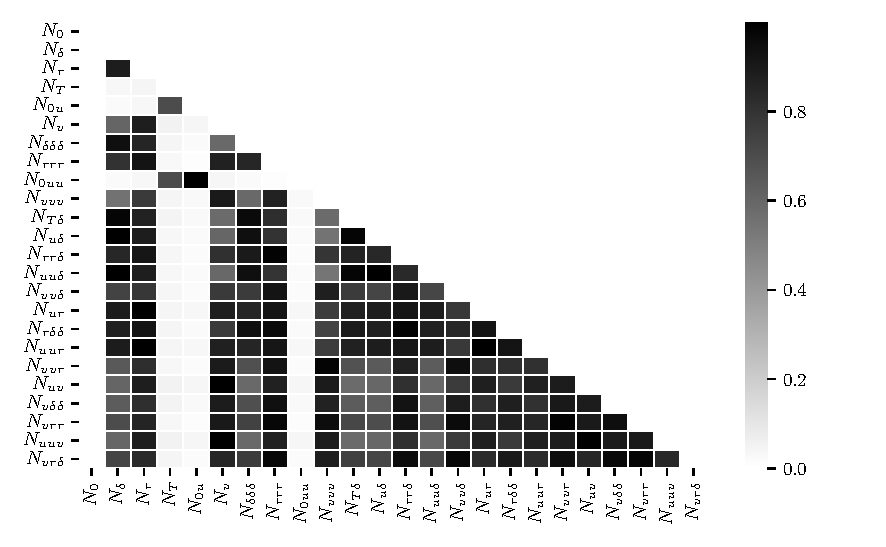
\includegraphics[width=1.0\textwidth]{kappa/images/10.pdf}
\caption{Absolute correlation between the features in the wPCC yaw moment regression of AVMM.}\label{fig:ncorr}
\end{figure}
\begin{figure}[h]
    \centering

    \begin{subfigure}[b]{\textwidth}
        \includegraphics[width=0.90\textwidth]{kappa/images/11.pdf}
        \caption{Track plots.}\label{fig:track-plot-testing-sim}
    \end{subfigure}
    \vfill
    \begin{subfigure}[b]{\textwidth}
        \includegraphics[width=0.90\textwidth]{kappa/images/12.pdf}
        \caption{Time series.}\label{\detokenize{06.10_results_wpcc:fig-testing-sim}}
    \end{subfigure}
        
    \caption{Turning circle test case for wPCC from model test and simulations.}
    \label{fig:enter-label}
\end{figure}

%\includegraphics[width=0.90\textwidth]{kappa/images/11.pdf}
%\caption{Turning circle test case for wPCC, track plots from model test and simulation.}\label{fig:track-plot-testing-sim}
%\end{figure}
%\begin{figure}[ht]
%\centering
%\includegraphics[width=0.90\textwidth]{kappa/images/12.pdf}
%\caption{Turning circle test case for wPCC, time series from model test and simulation.}\label{\detokenize{06.10_results_wpcc:fig-testing-sim}}\end{figure}
\FloatBarrier

The corresponding final prediction of the turning circle test for the KVLCC2 test case is shown in \autoref{fig:fig-kvlcc2-track-plot-testing-sim}. The prediction was conducted using simulation with the MAVMM trained on the training and validation datasets. Monte Carlo simulations with alternative realizations of the regression are also displayed in this figure. The alternative realizations are very similar to the model with mean values of the regression (black line).
The predicted advance and tactical diameters differ by 2\% and 5\%.
\begin{figure}[h]
    \centering

    \begin{subfigure}[b]{0.80\textwidth}
        \includegraphics[width=\textwidth]{kappa/images/17.pdf}
        \caption{Track plots.}
    \end{subfigure}
    \vfill
    \begin{subfigure}[b]{0.80\textwidth}
        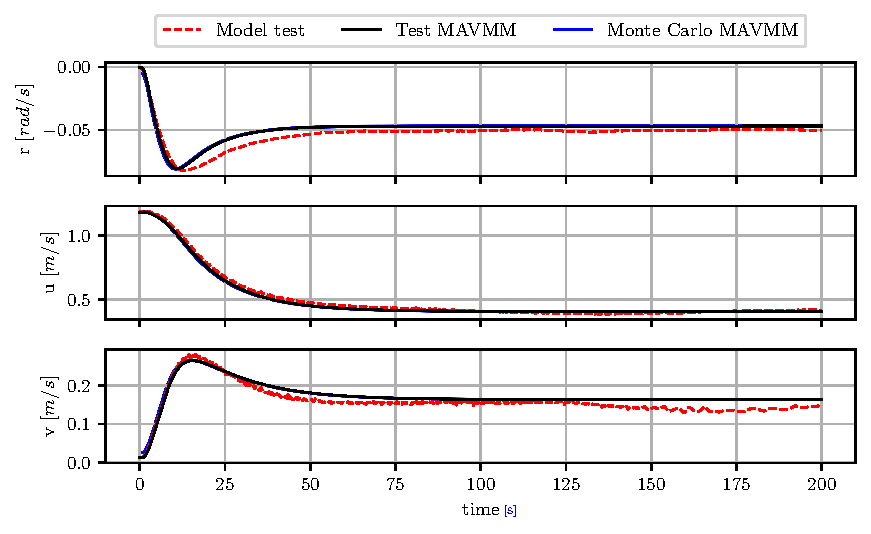
\includegraphics[width=\textwidth]{kappa/images/18.pdf}
        \caption{Time series}
    \end{subfigure}
        
    \caption{Comparison between the predicted turning circle test with MAVMM trained on HSVA data and MARIN model test results for KVLCC2.}
    \label{fig:fig-kvlcc2-track-plot-testing-sim}
\end{figure}
\section{Summary of Paper \ref{pap:physics}}
\subsection*{"\nameref{pap:physics}"}
\subsection*{Scope and motivations}
Minimizing the number of derivatives is often a good idea to avoid overfitting irrelevant data, following the prejudice approach that ''Nature is simple'' \cite{ljungPerspectivesSystemIdentification2010}. However, this could also lead to model structures with limited applicability, as certain regression terms may only become significant in special conditions like sailing in wind \cite{abkowitzMEASUREMENTHYDRODYNAMICCHARACTERISTICS1980}.

It was shown in Paper \ref{pap:pit} that it is possible to identify a model from calm water free running model test with inverse dynamics regression (\autoref{sec:IDR}) together with a cross validation technique to ensure good generalization so that the model can predict other kinds of maneuvers with very good accuracy. However, it was soon discovered that these models did not generalize well when wind forces were added to the simulations. This problem was addressed in Paper \ref{pap:physics}.

Paper \ref{pap:physics} uses two modular manoeuvring models. One of the models is a physics uninformed (PU) model which was a completely data driven model, similarly to the models used in the previous paper (Paper \ref{pap:pit}).
The other model was a physics informed (PI) model, where prior knowledge about rudder hydrodynamics has been added to guide the identification towards a more physically correct model. 
The models had identical prediction models for the hull and propeller forces but different models for the rudder forces. The PI model had a deterministic semi-empirical rudder model. The PU model had a data-driven mathematical rudder model. Except for the changed rudder models, the ship manoeuvring models were similar to the MMG model \cite{yasukawaIntroductionMMGStandard2015}, with some minor enhancements; The surge velocity was for instance expressed as a perturbed velocity (see \autoref{sec:prime_system}) allowing for higher order resistance coefficients.

A brief description of the workflow of Paper \ref{pap:physics} is shown in \autoref{fig:methodology}.
The PI and PU models were identified in free-running model tests using inverse dynamics and regression. To assess physical correctness, a reference model was established, where the PI model was instead identified on a VCT data set. This reference model, based on CFD, was assumed to be a sufficiently correct representation of the ship's physics.
Verification and comparisons between the models were carried out in the free-sailing model tests.
\begin{figure}[h]
  \centering
  %\includesvg[width=\columnwidth, pretex=\scriptsize, height=12cm]{figures/methodology2.svg}
  \includesvg[width=0.8\textwidth, pretex=\centering\fontsize{7.5}{8}]{kappa/images/methodology2.svg}
  \caption{Research workflow, describing how the reference model is identified with regression of VCT data and the PI and PU models are identified with regression of inverse dynamics forces from model tests. Results are then gathered to assess the parameter drift, physical correctness and generalization of the models.}
  \label{fig:methodology}
\end{figure}
It was investigated if the introduction of a deterministic semi-empirical rudder model in the PI model would reduce the multicollinearity and enhance the generalization.

\FloatBarrier
\clearpage
\subsection*{Results and concluding remarks}
Force predictions using reference, PI, and PU models for the states during one of the zigzag10/10 tests with wPCC were compared with the inverse dynamics forces for the same test in \autoref{fig:ID_zigzag10}. The PI and PU models predicted the same total yawing moment $N_D$ and sway force $Y_D$ as the reference model. However, the decomposition of this total yawing moment into components of the hull $N_H$ and the rudder $N_R$ differed significantly between the PU model and the PI and reference models, which were quite similar to each other.

\begin{figure}[h] \centering 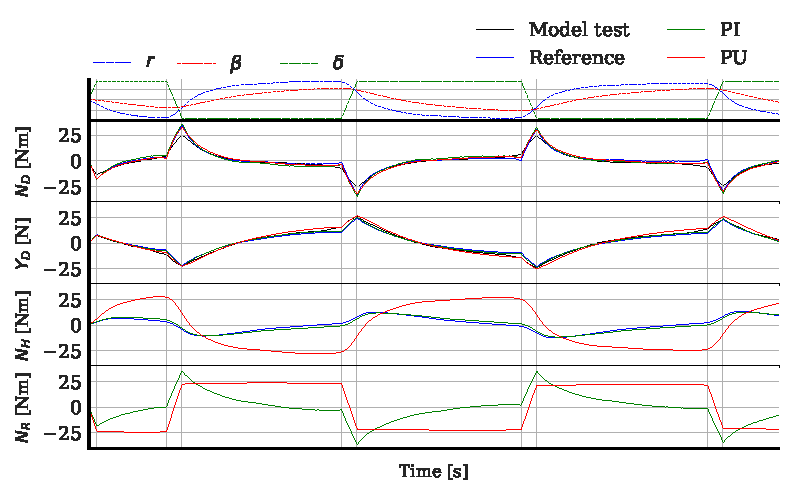
\includegraphics[width=0.9\textwidth]{kappa/images/results.ID_zigzag10.pdf} \caption{ID estimations of $Y_D$ and $N_D$ during a zigzag10/10 model test compared with model predictions.} \label{fig:ID_zigzag10} \end{figure}

The hull forces can be further decomposed into contributions from the drift of the vessel, through the sway velocity $v$, and contributions from the yaw rate $r$, as shown in \autoref{fig:ID_regression_N_decomposition}. It appears that almost all the yawing moments $N_H$ depend on $r$ for the PU model, and almost all the sway force $Y_H$ is generated by $v$. This contrasts with the other two models, where both $v$ and $r$ contribute to $N_H$ and $Y_H$.

\begin{figure}[h] \begin{center} \includesvg[width=0.9\textwidth]{kappa/images/results.hull_force_decomposition_zigzag20.svg} \caption{Decomposition of hull forces and moments during a zigzag20/20 test for parameters related to drift, yaw rate, and the prediction models.} \label{fig:ID_regression_N_decomposition} \end{center} \end{figure}

Thus, the PU model not only has an incorrect decomposition between rudder and hull forces, but it also incorrectly decomposes the drift and yaw rate contributions within the hull force model. However, this is not a significant problem during the zigzag tests, where the drift and yaw rate are highly correlated, as seen from the phase plot in \autoref{fig:phase_portrait}. This correlation can also explain why the completely data-driven model from the previous paper (Paper \ref{pap:pit}) achieves such good results despite the erroneous decomposition.

\begin{figure}[h] \centering \includesvg{figures/multicollineraity.multicollinearity.svg} \caption{Phase portrait showing the combination of drift angle and yaw rate for zigzag10/10 and zigzag20/20 wPCC model tests.} \label{fig:phase_portrait} \end{figure}

However, when the ship is exposed to wind, causing changes in drift, the erroneous decomposition of the PU model becomes apparent, as shown in \autoref{fig:result_wind_state}. The PI model aligns better with the reference model in the wind state. Introducing a semi-empirical rudder model seems to have guided the identification toward a more physically accurate model, with lower multicollinearity and better generalization from calm water zigzag tests to wind conditions.

\begin{figure}[h!] 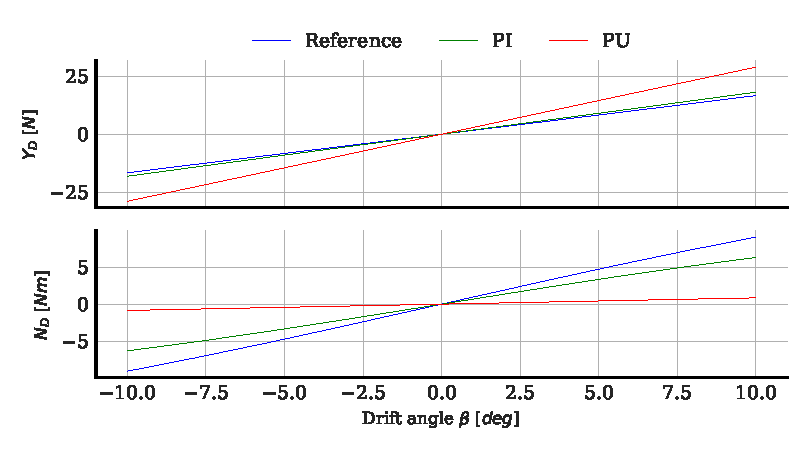
\includegraphics[width=\textwidth]{kappa/images/result_wind_state.forces.pdf} \caption{Total sway force and yawing moment from the wPCC models at various drift angles.} \label{fig:result_wind_state} \end{figure}

\FloatBarrier \clearpage
\section{Summary of Paper \ref{pap:vct}}
\subsection*{"\nameref{pap:vct}"}
\subsection*{Scope and motivations}
The objective of paper \ref{pap:vct} was to propose a parametric model structure based on physical insights from VCT and FT inverse dynamics. The reference model from Paper \ref{pap:physics} was assumed to be close to the physically correct true model of ship manoeuvring dynamics. This model was developed with VCT, which is based on physical first principles through CFD calculations. Paper \ref{pap:vct} investigated the identification of manoeuvring with VCT more closely, with the aim of achieving a model that more accurately reflected the true system.

Manoeuvring models were developed for the two WAPS test cases with large rudders. The models were identified by conducting a VCT to obtain hydrodynamic damping coefficients and by conducting pure yaw and pure sway tests in FNPF to obtain the added masses using the Fourier series method (see \autoref{sec:fourier}). The identified force models were compared with the inverse dynamics forces of the zigzag tests to identify potential weaknesses within the models.

\subsection*{Results and main findings}
Propeller and rudder forces were measured during the FRMTs for Optiwise. It was found that these measured forces together with forces predicted with a hull sub module, identified from VCT data, could recreate the estimated inverse dynamics forces during zigzag maneuvers with sufficient accuracy. Much effort was therefore devoted to finding a rudder force prediction model that could recreate the rudder forces for Optiwise. A modified quadratic MMG rudder model was proposed (see \autoref{sec:MMG_rudder}) as an improved version of the original model \cite{yasukawaIntroductionMMGStandard2015}. 
\autoref{fig:MMG_quadratic} shows the Optiwise rudder force $Y_R$ for the various VCT test types (see \autoref{sec:VCT}) plotted against the effective rudder angle $\beta_R$. The original MMG rudder model has a constant flow straightening factor $\gamma_{Rpos}$ for positive $\beta_R$ and another constant flow straightening factor $\gamma_{Rneg}$ for negative $\beta_R$. The proposed quadratic formulation has two additional parameters, $\gamma_{R2pos}$ and $\gamma_{R2neg}$, that allow the flow straightening to vary with $\beta_R$ that better fits the VCT data.
\begin{figure}[h]
     \centering
     \begin{subfigure}[b]{0.49\textwidth}
         \centering
         \includesvg[width=1\textwidth]{figures/results_optiwise_VCT.Y_R_MMG_original.svg}
        \caption{Original MMG rudder model.}
        \label{fig:Y_R_MMG_original}
     \end{subfigure}
     \hfill
     \begin{subfigure}[b]{0.49\textwidth}
         \centering
         \includesvg[width=1\textwidth]{figures/results_optiwise_VCT.Y_R_MMG_quadratic.svg}
        \caption{Modified quadratic MMG rudder model.}
        \label{fig:Y_R_MMG_quadratic}
     \end{subfigure}
    \caption{Rudder force during the VCT tests as a function of the effective inflow angle for the original MMG model and the modified quadratic MMG model.}
    \label{fig:MMG_quadratic}
\end{figure}

The rudder forces during the Optiwise FRMTs were predicted and compared with the corresponding measured forces, as shown in \autoref{fig:rudder_forces}. Although there were some minor deviations during the zigzag10/10 test, there was generally good agreement between the predictions and measurements. VCT calculations of some of the states during the manoeuvres have also been added to this comparison, which also show good agreement.
\begin{figure}[h]
    \centering
    \begin{subfigure}[b]{\textwidth}
        \centering
        \includesvg{figures/results_optiwise_ID.rudder_forces_zigzag 10_10.svg}
        \caption{Zigzag10/10 to port.}
        \label{fig:ID_measured_rudder_zigzag_10_10}
    \end{subfigure}
     \vfill
    \begin{subfigure}[b]{\textwidth}
        \centering
        \includesvg{figures/results_optiwise_ID.rudder_forces_zigzag 20_20.svg}
        \caption{Zigzag20/20 to starboard.}
        \label{fig:ID_measured_rudder_zigzag_20_20}
    \end{subfigure}
    \caption{Rudder forces during the zigzag tests compared to predictions with the MMG models.}
    \label{fig:rudder_forces}
\end{figure}

The total forces during the zigzag tests were also predicted, including the hull and rudder models. \autoref{fig:ID_optiwise20}  shows a comparison between the predicted forces and FRMT inverse dynamics forces. VCT calculations of some of the states during the manoeuvres have also been added to this figure, which agrees well with the model predictions.
However, deviations were observed for the sway force $Y_D$ within three seconds after the rudder changes at t = 11--14 s and t = 35--38 s, for the zigzag10/10 and t = 11--14 s, t = 35--38 s, t = 64 s, for the zigzag20/20. The model and state VCT calculations predict a straighter line in the $Y_D$ time series near these deviation points. No reasonable explanation for these deviations has been found, and filtration errors in the EKF were ruled out as a possible explanation.
\begin{figure}[h]
    \centering
    \begin{subfigure}[b]{\textwidth}
        \centering
        \includesvg{figures/results_optiwise_ID.zigzag 10_10.svg}
        \caption{Zigzag10/10 to port.}
        \label{fig:ID_MMG_zigzag_10_10}
    \end{subfigure}
     \vfill
    \begin{subfigure}[b]{\textwidth}
        \centering
        \includesvg{figures/results_optiwise_ID.zigzag 20_20.svg}
        \caption{Zigzag20/20 to starboard.}
        \label{fig:ID_MMG_zigzag_20_20}
    \end{subfigure}
    \caption{Inverse dynamics forces during the zigzag tests compared to predictions with the MMG models.}
    \label{fig:ID_optiwise20}
\end{figure}

Closed loop simulations were also conducted, as shown in \autoref{fig:sim_optiwise}, and exhibited strong agreement for the zigzag20/20 tests and a slightly lower agreement for the zigzag10/10 tests.
It can therefore be concluded for the Optiwise case that
the VCT data contained correct damping forces during the maneuvers, which were well
described by the chosen model structure, including the proposed rudder model, and that the method used to determine added masses produced reasonable values.
\begin{figure}[h]
     \centering
     \begin{subfigure}[b]{0.49\textwidth}
         \centering
         \includesvg{figures/results_optiwise_ID.closed loop zigzag 10_10 port.svg}
         %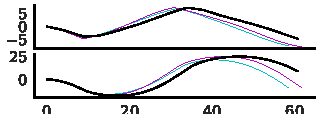
\includegraphics[]{figures/results_optiwise_ID.closed loop zigzag 10_10 port.pdf}
        \caption{Zigzag10/10 to port.}
        \label{fig:sim_optiwise_10_port}
     \end{subfigure}
     \hfill
     \begin{subfigure}[b]{0.49\textwidth}
         \includesvg{figures/results_optiwise_ID.closed loop zigzag 10_10 stbd.svg}
         %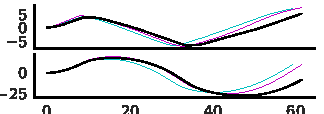
\includegraphics[]{figures/results_optiwise_ID.closed loop zigzag 10_10 stbd.pdf}
        \caption{Zigzag10/10 to starboard.}
        \label{fig:sim_optiwise_10_stbd}
     \end{subfigure}
     \vfill
     \begin{subfigure}[b]{0.49\textwidth}
         \centering
         \includesvg{figures/results_optiwise_ID.closed loop zigzag 20_20 port.svg}
         %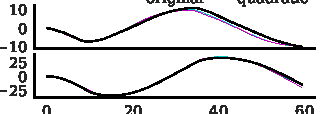
\includegraphics[]{figures/results_optiwise_ID.closed loop zigzag 20_20 port.pdf}
        \caption{Zigzag20/20 to port.}
        \label{fig:sim_optiwise_20_port}
     \end{subfigure}
     \hfill
     \begin{subfigure}[b]{0.49\textwidth}
         \includesvg{figures/results_optiwise_ID.closed loop zigzag 20_20 stbd.svg}
         %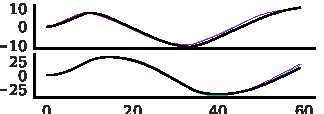
\includegraphics[]{figures/results_optiwise_ID.closed loop zigzag 20_20 stbd.pdf}
        \caption{Zigzag20/20 to starboard.}
        \label{fig:sim_optiwise_20_stbd}
     \end{subfigure}
     
        \caption{Comparison of zigzag tests between Optiwise experiments (black) and simulations with the MMG original (cyan) and MMG quadratic (purple).}
        \label{fig:sim_optiwise}
\end{figure}
%\input{kappa/04.10_discussion}






%%%%%%%%%%%%%%%%%%%%%%%%%%%%%%%
%%%%%%%%%%%%%%%%%%%%%%%%%%%%%%%
\chapter{Discussion\label{ch:discussion}}
%%%%%%%%%%%%%%%%%%%%%%%%%%%%%%%
This thesis has demonstrated that identifying parametric manoeuvring models from standard manoeuvres is challenged by high multicollinearity among many model parameters. This issue is well-documented; \textcite{yoonIdentificationHydrodynamicCoefficients2003} highlighted the difficulties in separately determining regression coefficients, and \textcite{wangQuantifyingMulticollinearityShip2018} discussed how multicollinearity can lead to parameter drift, resulting in unphysical models, as shown in this thesis.

\autoref{fig:handle_multicollinearity} presents a proposed flowchart for mitigating multicollinearity, addressing the challenges of correctly separating hull and rudder forces, as well as drift and yaw rate-dependent forces.
It was shown in Paper \ref{pap:physics} that a more accurate separation between hull and rudder forces can be achieved by introducing a deterministic semi-empirical rudder model, resulting in a more physically accurate model. Another effective approach is to measure the rudder forces, which yielded excellent results for the Optiwise test case in Paper \ref{pap:vct}.
\begin{figure}[h]
    
    \centering
        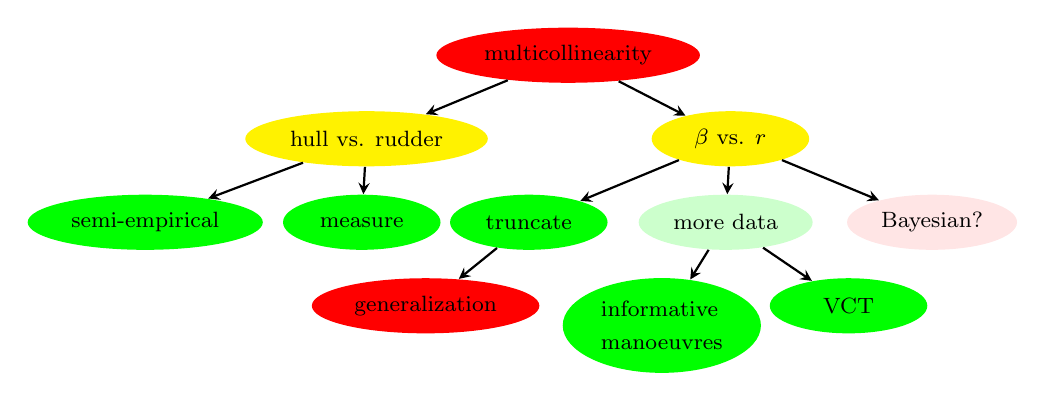
\begin{tikzpicture}[node distance=1.5cm]
    
    \node (multicollinearity) [problem] {\footnotesize multicollinearity};
    \node (hull_vs_rudder) [item, below left of=multicollinearity, xshift=-1.5cm] {\footnotesize hull vs. rudder};
    \node (beta_vs_r) [item, below right of=multicollinearity, xshift=1.0cm] {\footnotesize $\beta$ vs. $r$};
    
    \node (semi_empirical) [solution, below left of=hull_vs_rudder, xshift=-1.75cm] {\footnotesize semi-empirical};
    \node (rudder_measure) [solution, below left of=hull_vs_rudder, xshift=1cm] {\footnotesize measure};
    \node (truncate) [solution, below left of=beta_vs_r, xshift=-1.5cm] {\footnotesize truncate};

    \node (generalization) [problem, below left of=truncate, xshift=-0.25cm] {\footnotesize generalization};

    \node (more_data) [wish, below left of=beta_vs_r, xshift=1cm] {\footnotesize more data};
    \node (future) [future, below right of=beta_vs_r, xshift=1.5cm] {\footnotesize Bayesian?};
        
    \node (informative_manoeuvres) [solution, below left of=more_data, xshift=0.25cm, yshift=-0.25cm, align=left] {\footnotesize informative \\ \footnotesize manoeuvres};
    \node (VCT) [solution, below right of=more_data, xshift=0.50cm] {\footnotesize VCT};
    
    
    %Connect
    \draw [arrow] (multicollinearity) -- (hull_vs_rudder);
    \draw [arrow] (multicollinearity) -- (beta_vs_r);

    \draw [arrow] (hull_vs_rudder) -- (semi_empirical);
    \draw [arrow] (hull_vs_rudder) -- (rudder_measure);
    
    \draw [arrow] (beta_vs_r) -- (truncate);
    \draw [arrow] (beta_vs_r) -- (more_data);
    \draw [arrow] (beta_vs_r) -- (future);

    \draw [arrow] (more_data) -- (VCT);
    \draw [arrow] (more_data) -- (informative_manoeuvres);
    
    \draw [arrow] (truncate) -- (generalization);
        
    
    \end{tikzpicture}
    \caption{Flowchart for mitigating multicollinearity based on the research presented in this thesis.}
    \label{fig:handle_multicollinearity}
\end{figure}

Mitigating multicollinearity between drift and yaw rate-dependent parameters during standard manoeuvres is more challenging. \textcite{abkowitzMEASUREMENTHYDRODYNAMICCHARACTERISTICS1980}, \textcite{luoParameterIdentificationShip2016}, \textcite{xuUncertaintyAnalysisHydrodynamic2019}, \textcite{liuPhysicsinformedIdentificationMarine2024}, and Paper \ref{pap:pit} addressed this by truncating polynomials using various methods to select which parameters to remove. This approach is valid if the truncation method correctly identifies which parameters are identifiable from the data. However, model generalization inevitably suffers when parameters are removed, as certain regression terms may only become significant under specific conditions, such as sailing in wind. Truncated models may perform well when simulating conditions similar to the data, such as other standard manoeuvres, but excessive extrapolation should be avoided, as shown in Paper \ref{pap:physics}.

More informative data are needed to mitigate multicollinearity without reducing model generalization. \textcite{yoonIdentificationHydrodynamicCoefficients2003} emphasized the importance of designing experiments that ensure persistence of excitation. They suggested using specific input scenarios that maximize data information content, such as D-optimal designs. \textcite{wangOptimalDesignExcitation2020} and \textcite{millerShipModelIdentification2021} proposed using a pseudo-random sequence (PRS) for this purpose. These manoeuvres require more space than a model test basin provides, necessitating full-scale ship tests at sea or radio-controlled models on a lake.

Another option for gathering more informative data is conducting VCT calculations. Paper \ref{pap:vct} demonstrated that a physically accurate model can be identified in this way, effectively overcoming the multicollinearity problem while maintaining good model generalization.

If a VCT is infeasible, prior knowledge of drift and yaw rate forces can be incorporated, akin to the semi-empirical rudder model. \textcite{chillcceDatadrivenSystemIdentification2023} used a constrained least-squares algorithm, defining the sign and boundaries of the hydrodynamic derivatives based on prior knowledge from VCT. \textcite{taimuri6DoFManeuveringModel2020} proposed calculating hydrodynamic derivatives from semi-empirical formulas combined with corrections from a reference ship. Bayesian modeling offers a more refined approach to expressing prior knowledge as prior probability densities. \textcite{xueHydrodynamicParameterIdentification2020} used a Bayesian approach for parameter identification in manoeuvring models, employing an optimizer to suggest priors. A more accurate, though demanding, method would be to specify priors based on the estimation of hydrodynamic derivatives from many ships, which could be an interesting topic for future work, as discussed in further detail in \autoref{ch:future_work}.

%%%%%%%%%%%%%%%%%%%%%%%%%%%%%%%
%%%%%%%%%%%%%%%%%%%%%%%%%%%%%%%
\chapter{Discussion and conclusions\label{ch:conclusions}}
%%%%%%%%%%%%%%%%%%%%%%%%%%%%%%%
% The conclusions of the stated objectives...

The main conclusions are presented in this section with respect to the main objective of this thesis:
% Objective: 
\begin{quote} 
\vspace{0.1cm}
\objective \\
\vspace{-0.3cm}
\end{quote}
\noindent The conclusions are categorized by the goals that comprise this objective.

\subsubsection*{\normalfont \color{black} \textbf{Roll model}}
The first goal of the thesis was to use model test data to develop a model for the calm water rigid body ship dynamics in the roll degree of freedom. 
Three candidate models were considered:
\vspace{5pt}
\begin{itemize}
    \setlength\itemsep{5pt}
    \item the linear roll motion model
    \item the quadratic roll motion model
    \item the cubic roll motion model
\end{itemize}
\vspace{5pt}
\noindent Data from 250 roll decay tests obtained from SSPA were used to evaluate these models. The linear model was not as accurate as the nonlinear models. The quadratic model was almost as accurate as the cubic model and is expected to have a higher degree of generalization with fewer parameters in the model. Therefore,  the quadratic model is the best description for the roll motion. 

Predictions with the original Ikeda's method were also conducted for some of the ships that exceeded the limits of the simplified Ikeda's method. These predictions were in much better agreement with the dampings from the model tests. These results indicate that the observed deviations with the simplified Ikeda's method are the result of extrapolation rather than errors inherent 
to the original Ikeda's method.

A grey-box correction model of the simplified Ikeda's method and a complete black-box model to predict ship roll damping were proposed in Paper \ref{pap:rolldamping}. The proposed models yield better predictions than the simplified Ikeda's method outside its limits and worse predictions within its limits. Applying corrections to the simplified Ikeda's method outside its limits is therefore not enough for obtaining useful roll damping predictions for modern ships; an additional course of action is necessary. Further research efforts must focus on updating and improving the simplified Ikeda's method.

\subsubsection*{\normalfont \color{black} \textbf{Manoeuvring model}}
The second goal of this thesis was to increase the complexity and uncertainty of the modelling by adding the surge, sway, and yaw degrees of freedom. This goal addresses the manoeuvring problem. 

It is demonstrated in Paper \ref{pap:pit} that the hydrodynamic derivatives within a manoeuvring model can be identified exactly in ideal conditions with no measurement noise and a perfect estimator. Such a result appears during the identification of parameters in a manoeuvring model on data from simulations with the same manoeuvring model.
System identification on actual model tests has the challenge of handling the measurement noise and the model uncertainty. A new system identification method has been proposed in Paper \ref{pap:pit}, where a preprocessor with an EKF and an RTS smoother are run in iteration for a set of candidate manoeuvring models to handle both the measurement noise and model uncertainty. System identification with the proposed pre-processor has higher accuracy than when low-pass filters are applied. Parameter estimation with no filter or a low-pass filter with the wrong settings result in inaccurate estimations. 

The linearization in the EKF may threaten stability, which can be a problem for sparse time series with longer time steps. This was not a problem for the present test cases, with very high frequency data (100 Hz). 
Using the unscented Kalman filter (UKF) instead of the EKF can resolve stability issues . This resolution has not been examined further in this thesis.

Multicollinearity was a significant problem with the AVMM for both the wPCC and KVLCC2 data. Consequently, some of the regressed hydrodynamic derivatives in the AVMM have unphysically large values and substantial uncertainties. The model is still mathematically correct; the regressed polynomials fit the training data well. The regressed polynomial could be the sum of large counteracting coefficients. The model is effective when the states are similar to the training data. When extrapolating, the balance between these massive derivatives may be disturbed, which quickly yields significant extrapolation errors. This behavior occurred for the wPCC test case when predicting forces and moments with the AVMM on unseen validation data; it is a documented problem \cite{ittc_maneuvering_2008}.
The MAVMM has fewer hydrodynamic derivatives with lower multicollinearity and minor extrapolation errors. Including propeller thrust in the manoeuvring model made it possible to obtain high accuracy with fewer hydrodynamic derivatives. An additional concern with a high number of parameters in a model is that the standard manoeuvres used in this paper do not follow the aspect of persistence of excitation. As a result, some of the hydrodynamic derivatives might not be identifiable \cite{revestido_herrero_two-step_2012}. For instance, the model is exposed to only two rudder angles in the majority of the data during the zigzag tests. A series of step responses used in \cite{miller_ship_2021} provides a better excitation, but requires a large amount of space. Wider space is possible during lake experiments, but not in a narrow basin. The model generalization therefore must be addressed, as seen in the next section.

\subsubsection*{Model generalization} 
The third goal of this thesis was model generalization. In order to be of practical use in an Internet of Ships (IoS) application, the models must be able to make predictions outside the domain covered by the available data. A model development process for manoeuvring models with a high degree of generalization was proposed in Paper \ref{pap:pit}.
The process was executed along with the proposed parameter estimation technique on the wPCC and KVLCC2 test cases. Turning circles where predicted with high accuracy on models trained on zigzag tests. This result indicates that the models have a high degree of generalization because the turning circles have much larger rudder angles, drift angles, and yaw rates compared to the training zigzag tests. 

%%%%%%%%%%%%%%%%%%%%%%%%%%%%%%%
%%%%%%%%%%%%%%%%%%%%%%%%%%%%%%%
\chapter{Future work\label{ch:future_work}}
%%%%%%%%%%%%%%%%%%%%%%%%%%%%%%%
% Loosen up on the assumptions?
%Use a hyphen if "long-term" is an adjective.

\noindent The rigid body assumption during maneuvers is reasonable considering the relatively low accelerations and bending of the hull girder during maneuvers, at least in the absence of waves. However, there are other assumptions and limitations that can pave the way for future research, as described below.

\subsection*{Only data from standard test types such as turning circles or zigzag tests were used in this thesis, since they are commonly available for ships}
It has been shown in this thesis that identifying a physically correct manoeuvring model from data with only standard maneuvers is very difficult, due to high multicollinearity and insufficient persistence of excitation. 
It was shown that prior knowledge about manoeuvring hydrodynamics embedded in the model structure together with good semi-empirical formulas can help to mitigate these problems.
However, it does not solve the problem completely. More informative data is needed to identify a fully physically correct model which could be obtained with other types of maneuvers, such as pseudo random binary sequence (PRBS) \cite{yoonIdentificationHydrodynamicCoefficients2003,wangOptimalDesignExcitation2020}. Studies of system identification on these kinds of informative maneuvers have mainly been conducted with simulated data. Collecting experimental data for these informative maneuvers would be a great contribution. The maneuvers require more space than is available in a model test basin. \textcite{millerShipModelIdentification2021} conducted such tests on a lake and pointed out that they are very difficult and time-consuming to carry out. 
More work is needed to establish reliable experimental research data from maneuvers in which all modes of the manoeuvring dynamics of the ship are excited, which could perhaps be conducted with one of the more well-researched test cases, such as for instance KVLCC2. 

\subsection*{Bayesian modeling}
Compared to the methods used in this thesis to incorporate prior knowledge about ship hydrodynamics, Bayesian modeling offers a more sophisticated approach by expressing prior knowledge as prior probability densities. Informative priors can guide parameter identification towards hydrodynamic derivatives that are physically reasonable, based on prior knowledge from similar ships, even for standard manoeuvres that lack persistence of excitation. However, developing informative priors for hydrodynamic derivatives would require significant research efforts, such as creating a comprehensive database of identified manoeuvring models for numerous ships. This effort would enable the identification of models with much better generalization from standard manoeuvres. Additionally, Bayesian modeling with informative hydrodynamic priors could have valuable applications in the system identification of full-scale ship operations and autonomous ships. 

\subsection*{Calm water assumption}
The sea is never calm, so this assumption within manoeuvring is a great simplification of the real conditions encountered by ships. Loosening up on this assumption would make system identification much harder. The fluid memory effect would have to be handled and the constant added mass assumption can no longer be justified. A different approach to what has been presented in this thesis would have to be adopted. A data-driven model for the viscous manoeuvring forces can perhaps be coupled with potential flow calculations in a similar way as it was done for the roll motion in Paper \ref{pap:ikeda}.  
    
\subsection*{The free surface effects and the influence of the roll were not included in the VCT data}
It was shown in the Paper \ref{pap:vct} that a manoeuvring model could be identified from VCT to predict standard maneuvers with good precision for one of the tested cases, but not for the other ship. 
It was argued that this was because the assumed neglection of the free surface and roll influence was not justified for this ship, which is a statement that would need further investigations to prove. A better understanding of when these assumptions can be applied is also needed.   
        


\renewcommand\bibname{References}
\printbibliography[heading=bibintoc]
\begin{appendices}
\renewcommand{\theequation}{\thechapter.\arabic{equation}}

\chapter{Initial estimates}
\label{app:initial_estimates}
The parameter estimation method requires an initial guessed linear manoeuvring model. Initial models for the two test cases have hydrodynamic derivatives that can be calculated with semi\-empirical formulas (\autoref{equation:05.01_case_studies:eqnr}-\autoref{equation:05.01_case_studies:eqyvdot}) taken from \cite{brixManoeuvringTechnicalManual1993}.

\begin{equation}\label{equation:05.01_case_studies:eqnr}
\begin{split}\displaystyle N_{r} = - \frac{\pi T^{2} \left(\frac{0.039 B}{T} - \frac{0.56 B}{L} + 0.25\right)}{L^{2}}\end{split}
\end{equation}\begin{equation}\label{equation:05.01_case_studies:eqnrdot}
\begin{split}\displaystyle N_{\dot{r}}' = - \frac{\pi T^{2} \left(\frac{0.017 B CB}{T} - \frac{0.33 B}{L} + 0.0833333333333333\right)}{L^{2}}\end{split}
\end{equation}\begin{equation}\label{equation:05.01_case_studies:eqnv}
\begin{split}\displaystyle N_{v} = - \frac{\pi T^{2} \left(0.5 + \frac{2.4 T}{L}\right)}{L^{2}}\end{split}
\end{equation}\begin{equation}\label{equation:05.01_case_studies:eqnvdot}
\begin{split}\displaystyle N_{\dot{v}}' = - \frac{\pi T^{2} \left(- \frac{0.04 B}{T} + \frac{1.1 B}{L}\right)}{L^{2}}\end{split}
\end{equation}\begin{equation}\label{equation:05.01_case_studies:eqxudot}
\begin{split}\displaystyle X_{\dot{u}}' = \frac{2.0 m}{L^{3} \rho \left(\pi \sqrt{\frac{L^{3}}{volume}} - 14\right)}\end{split}
\end{equation}\begin{equation}\label{equation:05.01_case_studies:eqyr}
\begin{split}\displaystyle Y_{r} = - \frac{\pi T^{2} \left(- \frac{0.08 B}{T} + \frac{2.2 B}{L} - 0.5\right)}{L^{2}}\end{split}
\end{equation}\begin{equation}\label{equation:05.01_case_studies:eqyrdot}
\begin{split}\displaystyle Y_{\dot{r}}' = - \frac{\pi T^{2} \left(- \frac{0.0033 B^{2}}{T^{2}} + \frac{0.67 B}{L}\right)}{L^{2}}\end{split}
\end{equation}\begin{equation}\label{equation:05.01_case_studies:eqyv}
\begin{split}\displaystyle Y_{v} = - \frac{\pi T^{2} \left(\frac{0.4 B CB}{T} + 1\right)}{L^{2}}\end{split}
\end{equation}\begin{equation}\label{equation:05.01_case_studies:eqyvdot}
\begin{split}\displaystyle Y_{\dot{v}}' = - \frac{\pi T^{2} \left(- \frac{5.1 B^{2}}{L^{2}} + \frac{0.16 B CB}{T} + 1\right)}{L^{2}}\end{split}
\end{equation}
\end{appendices}
%  \end{refsection}
\cleardoublepage

%\printbibliography[heading=subbibintoc] % biblatex bibliography


% % % Preparations before Part II. In this part one chapter = one paper

\renewcommand{\chaptername}{Paper}
                              % write 'Paper' instead of 'Chapter' in the title

\setcounter{chapter}{0}       % reset chapter numbers after Part I


% Fix hyperlinks to chapters/papers after chapter counter reset, see
% http://tex.stackexchange.com/a/6099
\renewcommand\theHchapter{appendedPaper.\arabic{chapter}}

\renewcommand{\thesection}{\arabic{section}}
                              % exclude chapter number from section number
                              % Figures, Tables, etc are still prefixed by chapter number.
                              % For algorithms numbering see definition of
                              % \newfloat{algorithm} above.

\newcommand{\paper}[7]
% #1 Paper Title
% #2 Short Title for page headers (ToC has the full title)
% #3 Label for later (or earlier) \ref:s
% #4 Authors
% #5 Where published
% #6 Comment (like "reprinted with a kind permission" and "reformatted for uniformity")
% #7 File to input
{
  \chapter{#1\label{#3}}      % Title as Chapter
  \chaptermark{#2}            % Short title for the page header
  \thispagestyle{empty}       % no page numbers
  {\Large #4}\par             % authors
  \vspace{1cm}
  \noindent\emph{\Large #5}\par % where published
  \vspace{3cm}
  \noindent\emph{\Large #6}   % Comment
%  \cleardoublepage            % skip back side of the page
%  \thispagestyle{plain}       % no header above paper title
%  \begin{center}
%    {\Large \bfseries Paper~\thechapter. #1}\par % title again
%    \vspace{1pc}
%    #4 \par                   % authors again
%    \vspace{3pc}
%  \end{center}
%  \begin{refsection}          % start of biblatex's refsection for sub-bibliography
%  \input{#7}                  % paper itself, starting from abstract (no title)
%  \printbibliography[heading=subbibintoc] % biblatex bibliography
%  \end{refsection}            % end of biblatex refsection
}

\newcommand{\reformatted}{The paper was reformatted for uniformity, but otherwise is unchanged.}

\addtocontents{toc}{\cftpagenumbersoff{chapter}}

\setcounter{part}{1}
\part{Appended papers}        % in this part one chapter = one paper

% Example of using the command \paper defined above: 
\paper{Analysis of roll damping model scale data}
      {~}
      {pap:rolldamping}
      {\fullcite{alexanderssonAnalysisRollDamping2021}}
      {~}
      {~}
\newpage
%\includepdf[pages=2-]{paper1.pdf}

\paper{Prediction of roll motion using fully nonlinear potential flow and Ikeda's method}
      {~}
      {pap:ikeda}
      {\fullcite{alexanderssonPredictionRollMotion2021}}
      {~}
      {~}
\newpage
%\includepdf[pages=2-]{paper1.pdf}

\paper{System identification of {vessel} {manoeuvring} {models}}
      {~}
      {pap:pit}
      {\fullcite{alexanderssonSystemIdentificationVessel2022}}
      {~}
      {~}
\newpage
%\includepdf[pages=-]{paper2.pdf}

\paper{System identification of a physics-informed ship model for better predictions in wind conditions}
      {~}
      {pap:physics}
      {\fullcite{alexanderssonSystemIdentificationPhysicsinformed2024b}}
      {~}
      {~}
\newpage
%\includepdf[pages=-]{paper2.pdf}

\paper{Identification of manoeuvring models for wind-assisted ships with large rudders using virtual captive tests}
      {~}
      {pap:vct}
      {~}
      {~}
      {~}
\newpage
%\includepdf[pages=-]{paper2.pdf}

\end{document}
